\chapter[Matematické modelování epidemií]{Matematické modelování epidemií: historie a současnost}
\label{Typy_modelu}

\textit{Luděk Berec}
\vspace{15mm}

\section*{Úvod}

Věda je systematický proces poznávání světa, kdy neustále konfrontujeme konkurenční hypotézy o tom, jak svět funguje, s tím, co pozorujeme. Získáme-li takto určitou představu o fungování nějaké části reality, můžeme se pokusit nahlédnout do budoucnosti a předpovědět její další možný vývoj. A máme-li možnost takových předpovědí, můžeme se pokusit blízkou budoucnost cíleně formovat. Blížíme-li se jako chodci k přechodu a v dálce vidíme přijíždět auto, máme určitou představu o tom, jak se auto přibližuje, že se z ničeho nic neobjeví před námi, a jsme většinou schopni odhadnout, kdy k nám dojede. Stejně tak to platí pro naši chůzi a odhad, kdy se dostaneme k přechodu. Pokud by naše předpověď znamenala střet, „vypočtenou“ budoucnost změníme, zastavíme a počkáme, až auto přejede, případně řidič zastaví. Ač nás to jistě ani nenapadlo, celou dobu, zahrnující posouzení situace, náhled do budoucnosti i její změnu, jsme modelovali.

Vědecké zkoumání světa tedy začíná hypotézou, představou o tom, jak svět funguje. Hypotézu, dosud neověřené tvrzení o fungování nějaké části reality, konfrontujeme s pozorováními. Tato pozorování už můžeme mít k dispozici (snažíme se něco vysvětlit), nebo je v návaznosti na naši hypotézu teprve získáme (snažíme se něco objevit). Z „potvrzených“ hypotéz následně budujeme teorii, obecné principy fungování určité části světa dostatečně podpořené pozorováními. Mezi nejznámější teorie patří například Einsteinova teorie relativity či Darwinova teorie přirozeného výběru. A právě zde mohou do hry vstoupit modely. Modely jako zjednodušené reprezentace určité části reality, vytvořené za určitým cílem, nejsou ani hypotézy, ani teorie, nýbrž základní nástroje či arbitři při konfrontacích hypotéz a pozorování. Vyšetřování každé letecké katastrofy znamená formulaci mnoha hypotéz. A řadu těchto hypotéz ověřujeme tak, že postavíme zmenšenou verzi (tedy model) určité části letadla, kde mohlo k příčině katastrofy dojít, a na ní se pak pokoušíme tyto hypotézy ověřit.

Matematické modely, tedy matematické reprezentace určité části světa, dnes hrají nezastupitelnou roli v řadě vědeckých disciplín a nejinak je tomu v epidemiologii. Jak si ukážeme v následující části, matematické modelování je součástí epidemiologie už více než 100 let. Během této doby plnilo nejrůznější úkoly, které na něj v různých situacích klademe: jako nástroj pro ověřování hypotéz, pro vysvětlení pozorovaných dat, pro pochopení základních principů infekční dynamiky, pro výpočet základních epidemiologických veličin, pro porozumění aktuálnímu chování specifických infekcí, pro předpovědi dalšího šíření infekcí, pro posouzení vlivu možných protiepidemických opatření či pro plánování vakcinačních strategií. Řadu těchto rolí hrály a stále hrají matematické modely i vzhledem k epidemii covid-19 po celém světě, a to včetně České republiky.

V této kapitole si představíme první historické kroky matematické epidemiologie, jak se také aktivitám spojeným s modelováním infekčních nemocí souhrnně říká, které formovaly a formují modelování epidemií dodnes. Naznačíme také těžkosti, které musí každý matematický modelář překonávat, chce-li modelovat konkrétní epidemii. Nakonec si stručně představíme model, který jsme vytvořili v rámci centra BISOP pro popis první vlny epidemie covid-19 na jaře roku 2020 v České republice, a ukážeme si některé jeho výsledky. Je dobré si uvědomit, že neexistuje jediný správný matematický model epidemie, dokonce že žádný model není správný, neboť každý model je nutně už z definice abstrakcí a zjednodušením reality. Určité modely mohou být pro zkoumání dané hypotézy lepší než jiné, avšak i ty v dané chvíli lepší mohou být nahrazeny jinými, máme-li k dispozici nové informace, data či změní-li se podmínky. Skvělým úvodem do problematiky modelů a modelování z filozofického i praktického hlediska jsou knihy \cite{GerleeLundh2016} a \cite{HilbornMangel1997}.

\section*{Historie a současnost matematické epidemiologie}

% \subsection*{Daniel Bernoulli a pravé neštovice}

\paragraph{Daniel Bernoulli a pravé neštovice:} První známé užití matematiky při řešení problému svázaného s infekční nemocí je spojeno s hledáním odpovědi na otázku, zda dlouhodobé přínosy variolace převáží nad okamžitými riziky. Variolace, původní metoda boje proti pravým neštovicím, spočívala v přenesení rozdrceného stroupku nebo tekutiny z puchýřku člověka nakaženého lehčí formou neštovic do kůže zdravého člověka s tím, že se u takového člověka vytvoří ochrana i proti těžší formě infekce. Tato metoda přišla do Evropy z Číny a Indie během 18. století, avšak nezískala přílišnou podporu. 

Na žádost francouzského matematika Maupertuise se otázkou přínosů versus\ rizik variolace začal zabývat švýcarský lékař, fyziolog, matematik, fyzik a biolog Daniel Bernoulli (1700--1782). Sestavil matematický model, který popisoval věkové rozložení počtu jedinců, kteří do daného věku pravými neštovicemi dosud neonemocněli, a jedinců, kteří se dožili daného věku a přitom už neštovice prodělali. Na základě dobových dat o populační struktuře vypočítal, že zatímco očekávaná délka života v populaci s pravými neštovicemi je 26 let a 7 měsíců, očekávaná délka života v populaci bez pravých neštovic je o zhruba 3 roky více (29 let a 8 měsíců). Následně odhadl, že variolace má z hlediska celé společnosti smysl, pokud je riziko úmrtí díky variolaci menší než 11\%, přičemž reálně docházelo k úmrtím pouze přibližně v 1 \% případů \cite{Bacaer2011}. Přesto tato metoda ve Francii plošnou podporu nakonec nezískala. Problém variolace navíc ztratil na významu o několik desítek let později, když Edward Jenner v roce 1798 objevil bezpečnější metodu: místo méně virulentní formy pravých neštovic použil neštovice kravské. A protože se kráva řekne latinsky \emph{vacca}, nazval Jenner svou metodu \emph{vakcinace}. 

Přestože byly pravé neštovice ve druhé polovině 20.\ století díky celosvětové kampani globálně vymýceny (zmíníme se o tom více v kapitole \ref{Ucinnost_ockovani}), dodnes se v literatuře objevují práce zabývající se modelováním šíření této infekce a boje proti ní, a to v souvislosti s možným bioterorismem \cite{Bozzette_etal2003,Longini_etal2007}.

Žádná vakcína není bez rizika. Platilo to pro variolaci u pravých neštovic stejně jako pro dnešní vakcíny proti covid-19. Opakovaně dnes slýcháme, že přínosy vakcín převažují nad jejich riziky. S touto tezí přišel už v roce 1760 Daniel Bernoulli, když proti sobě ve svém modelu postavil dlouhodobé výhody a okamžitá rizika variolace. Matematika sama však na tuto problematiku nestačí. Dostávají se zde totiž do určitého konfliktu zájmy jedince a zájmy společnosti. Z hlediska společnosti je jistě výhodné variolovat či očkovat, riziko nákazy každého z nás s vyšší proočkovaností populace nepochybně klesá. Každý jednotlivý naočkovaný člověk však může být právě ten, který si vytáhne Černého Petra negativních následků, či dokonce smrti. Matematické modely epidemií mohou řešit jen společenskou stránku tohoto konfliktu.

V souvislosti s pracemi Daniela Bernoulliho a Edwarda Jennera jsou zajímavé také dva jejich citáty. První z nich propagoval myšlenku, že je-li možné se k problému postavit matematicky, měli bychom tak učinit \cite{Bacaer2011}: \emph{Přál bych si, aby ve věci, která se tak bytostně týká lidské rasy, nebyla činěna žádná rozhodnutí bez znalostí, které může poskytnout sebemenší analýza a výpočet.} Edward Jenner pak po svém objevu vakcinace vyjádřil obavy, které během pandemie covid-19 v jistém smyslu pronásledovaly snad každého matematického modeláře snažícího se na své výsledky upozornit veřejnost, politiky a zástupce zdravotnictví \cite{JennerCitat}: \emph{Nevím, zda jsem přece jen neudělal chybu a nestvořil něco úděsného.}

%\subsection*{Ronald Ross a malárie}

\paragraph{Ronald Ross a malárie:} Dalším z průkopníků matematické epidemiologie byl Ronald Ross (1857--1932). Ross, vystudovaný lékař, se ve svém volném čase sám učil matematice. Po čase začal studovat malárii a dosáhl v této oblasti řady úspěchů, korunovaných ziskem Nobelovy ceny za fyziologii nebo lékařství v roce 1902. Mimo jiné prokázal, že se malárie přenáší nikoli pitím vody kontaminované komáry, nýbrž komářím bodnutím. Osobně v malarických oblastech proti komárům bojoval a propagoval myšlenku, že \emph{k vymýcení malárie postačí populaci komárů dostatečně zredukovat}. Při některých kampaních však tato metoda zdá se nefungovala, neboť ani po zredukování komářích populací prevalence nemoci příliš neklesla. Aby vyvrátil skepsi, že tato metoda příliš nefunguje, obrátil se Ross k matematice a vyvinul model malárie, doufaje, že rozličné výsledky různých protikomářích kampaní dokáže jednotně vysvětlit. 

\begin{figure}[h]
\begin{center}
	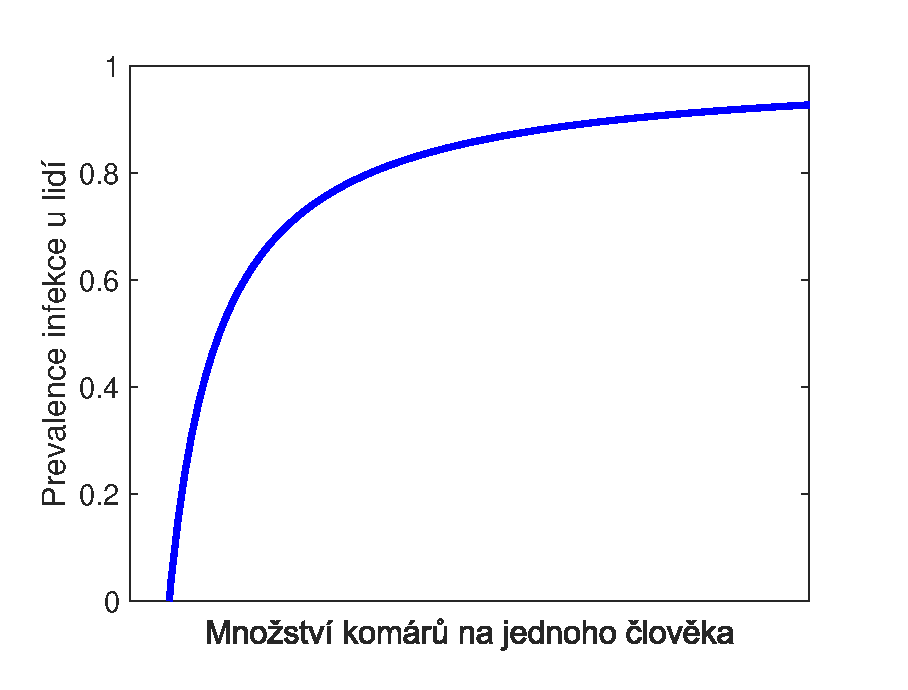
\includegraphics[width=0.6\textwidth]{pic/ross_plot.eps}
\end{center}
\caption{Pro eradikaci malárie není nutné vyhubit všechny komáry.}
\label{ross1}
\end{figure}

Pomocí svého modelu \cite{Smith_etal2012} Ross ukázal, že pokud počet komárů na jednoho člověka klesne pod určitou kritickou mez, infekce z populace postupně vymizí, kdežto v opačném případě se v populaci ustaví endemická rovnováha s určitou úrovní prevalence malárie (obr.\,\ref{ross1}). Prevalence malárie v endemické rovnováze přitom se zvyšujícím se množstvím komárů na jednoho člověka roste hyperbolicky (obr.\,\ref{ross1}). To znamená, že určitá daná změna velikosti komáří populace vede k relativně malé změně prevalence malárie, je-li populace komárů velká, a naopak k významné změně její prevalence, je-li populace komárů relativně malá. Úspěšné i zdánlivě neúspěšné eradikační kampaně proti komárům jsou tak založeny na stejném mechanismu, avšak jejich účinnost závisí na aktuálním stavu systému, tedy na aktuálním množství komárů na jednoho člověka. Tohoto vhledu bychom bez matematických modelů jen těžko dosáhli. Jedním z poučení z Rossova závěru může být to, že pokud v různých studiích má dané opatření různý dopad (příkladem zde může být v souvislosti s infekcí covid-19 mnohými různě vnímaná účinnost ne/zavírání škol), může existovat proměnná, vůči níž je efekt opatření různý, přitom však řízený stejným principem. 

Sám Ross, lékař s určitou znalostí matematiky, k modelování infekčních nemocí poznamenal \cite{Bacaer2011}: \emph{Vlastně celá epidemiologie, zabývající se změnami nemoci od jednoho okamžiku k druhému a od jednoho místa k jinému, má-li být pojata vědecky, musí být uchopena matematicky, a to bez ohledu na to, kolik proměnných je třeba vzít v úvahu. Říci, že nemoc je ovlivněna nějakým faktorem neznamená moc, pokud nejsme schopni kvantitativně odhadnout, do jaké míry každý z faktorů ovlivňuje celkový výsledek. A matematický přístup k řešení vlastně ve skutečnosti není nic jiného než pečlivé uvažování o daném problému.} Ross tak kromě jiného upozornil ještě na jeden, často opomíjený aspekt matematického modelování, a to nutnost přemýšlet o problému exaktně, jasně formulovat své hypotézy, předpoklady a znalosti o uvažovaném systému, a pomoci tak mimo jiné identifikovat nepřesnosti v uvažování a mezery ve znalostech, které o systému máme.     

Matematické modely se při studiu malárie a mnoha jiných vektory přenášených infekcí používají dodnes \cite{Gratz1999,Reiner_etal2012}. Původní Rossův jednoduchý model se dále vyvíjel a postupně zahrnoval stále větší detaily, např. věkovou strukturu komárů či detailnější epidemiologii malárie v obou populacích. V tomto byl jedním z největších následovníků Ronalda Rosse v polovině 20.\ století George Macdonald. Dvě skvělé přehledové studie mapující vývoj matematických modelů malárie představují práce \cite{Smith_etal2012} a \cite{Smith_etal2018}.

% \subsection*{A. G. McKendrick, W. O. Kermack a teorie epidemií}

\paragraph{A. G. McKendrick, W. O. Kermack a teorie epidemií:} Nástup systematického modelování v epidemiologii je spojen s prací A. G. McKendricka a W. O. Kermacka, kteří položili základy obecné teorie epidemií, jak ji známe dnes. Také McKendrick, opět vzděláním lékař, který mimo jiné doprovázel Ronalda Rosse při antikomáří kampani v Sieře Leone a zabýval se také vzteklinou, začal v určité chvíli studovat matematiku. Kermack byl vystudovaný chemik a s McKendrickem na modelování epidemií později spolupracoval. Z pohledu modelování epidemií je nejvýznamnějším dědictvím této dvojice dnes hojně skloňovaný SIR model, původně formulovaný jako stochastický model \cite{McKendrick1925} či model s procesy nakažení se a uzdravení se závislými na čase, který uplynul od okamžiku infekce (age-of-infection model) \cite{McKendrickKermack1927,YangBrauer2008}. Speciálním případem obou těchto modelů je pak klasický (deterministický) SIR model, jak jej nejčastěji známe dnes. Tento model dělí společnost do tří tříd: jedinci vnímaví či náchylní k infekci (třída $S$), aktuálně infekční jedinci (třída $I$) a jedinci dříve nemocní a nyní uzdravení (třída $R$). Přechod mezi těmito třídami řídí dva procesy: nakažení se, znamenající přechod z třídy $S$ do $I$, a uzdravení se, kdy jedinec přejde z třídy $I$ do $R$. Můžeme tak uvážit přírůstky či úbytky počtu jedinců v jednotlivých třídách během nějakého časového kroku, například jednoho dne: ze třídy $S$ odejdou jedinci, kteří se daný den nakazí, a tito nově nakažení jedinci se tak objeví ve třídě $I$, ze třídy $I$ pak odejdou jedinci, kteří se daný den uzdraví, a tito uzdravení jedinci se tak objeví ve třídě $R$. Nákaza přitom vzniká kontaktem vnímavého a infekčního jedince. Matematický model takového systému tedy může vypadat například takto (se SIR modelem se mnohem častěji setkáváme ve verzi se spojitým časem, a tedy ve tvaru systému diferenciálních rovnic, avšak pro větší názornost jej zde uvádíme ve verzi diskrétního času ve formě diferenčních rovnic):
\begin{equation}
\begin{array}{l}
\displaystyle{S[t+1] = S[t] - \beta \, \frac{S[t]\,I[t]}{N}}, \\[3ex]
\displaystyle{I[t+1] = I[t] + \beta \, \frac{S[t]\,I[t]}{N} - \gamma I[t]}, \\[3ex]
\displaystyle{R[t+1] = R[t] + \gamma I[t]},
\end{array}
\label{SIR1}
\end{equation}
kde $S[t]$ je počet vnímavých jedinců v čase $t$, $I[t]$ je počet infekčních jedinců v čase $t$, $R[t]$ je počet uzdravených jedinců v čase $t$, $N$ je konstantní velikost populace a parametry $\beta$ a $\gamma$ zjednodušeně řečeno určují míru nakažlivosti a uzdravování se. Typické řešení tohoto modelu ukazuje obr.\,\ref{kendrick1}. Zatímco vnímavých jedinců ubývá a uzdravených přibývá, počet aktuálně infekčních jedinců vytváří \emph{epidemickou vlnu}, známou z řady reálných epidemií \cite{Bell_etal2016,Finger_etal2019}. Právě schopnost SIR modelu tuto vlnu replikovat z něj dělá ten nejjednodušší model schopný kvalitativně popsat epidemie.  

SIR model je dnes základním stavebním kamenem takřka všech epidemických modelů. Kromě schopnosti reprodukovat epidemickou vlnu dokázal vysvětlit také další pozorování, v době McKendricka a Kermacka nejasné: proč epidemie zmizí dříve, než se nakazí všichni jedinci v populaci? Zkoumání této otázky mimo jiné vedlo k definici a pochopení významu veličiny, které říkáme \emph{(efektivní) reprodukční číslo $R$ neboli počet jedinců, které infekční jedinec nakazí}: počty nových případů infekce rostou, pokud $R>1$, a klesají, pokud $R<1$. Pro SIR model (\ref{SIR1}) je na počátku epidemie toto číslo rovno $\beta/\gamma$ a nazýváme jej \emph{základní reprodukční číslo} $R_0$, v dalším průběhu epidemie pak má časově proměnnou hodnotu $R = (\beta/\gamma)(S[t]/N) = R_0 \,S[t] / N$. Odtud mimo jiné plyne, že nových případů začne ubývat, jakmile podíl vnímavých jedinců v populaci, $S[t]/N$, klesne pod hodnotu $1/R_0$. Z modelu (\ref{SIR1}) lze také odvodit, že zpočátku bude počet aktuálně infekčních jedinců růst jako $I[t] \approx I[0]\,(1+\gamma\,(R_0-1))^t$, kde $I[0]$ je počet infekčních jedinců na startu epidemie. Tento vztah je matematickým popisem \emph{exponenciálního růstu}. Dále lze z modelu (\ref{SIR1}) odvodit, že prevalence infekce na vrcholu epidemie bude funkcí $R_0$ a že celkový počet nakažených po odeznění epidemie nebude $N$, nýbrž menší číslo opět závislé na $R_0$ (obr.\,\ref{kendrick1}). Ve všech těchto vztazích tedy vystupuje $R_0$, což je hlavní důvod, proč se vědci při vypuknutí každé epidemie po této hodnotě tak rychle pídí (paradoxně ve chvíli, kdy zatím není dostatečný počet nakažených). V takové chvíli zatím o chování infekce moc nevíme, a SIR model se tak zdá být tím nejpřirozenějším, s čím začít. 

\begin{figure}[h]
\begin{center}
	\begin{minipage}[m]{0.45\linewidth}
		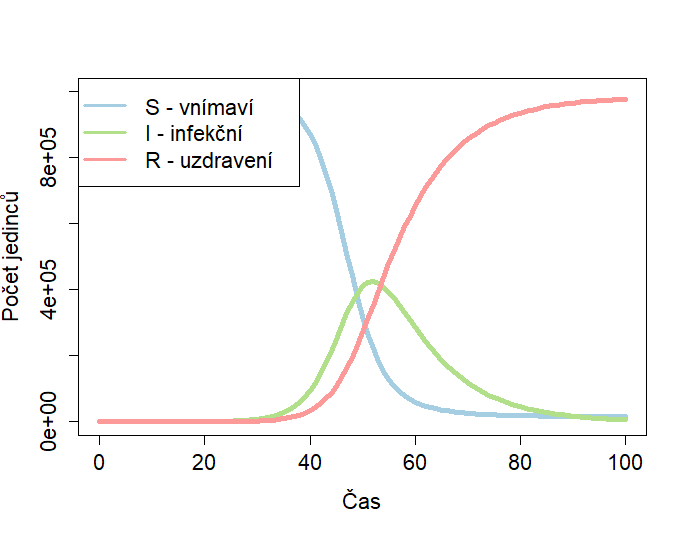
\includegraphics[width=0.99\textwidth]{pic/figsir1.png}
	\end{minipage}
	\hspace{2ex}
	\begin{minipage}[m]{0.45\linewidth}
		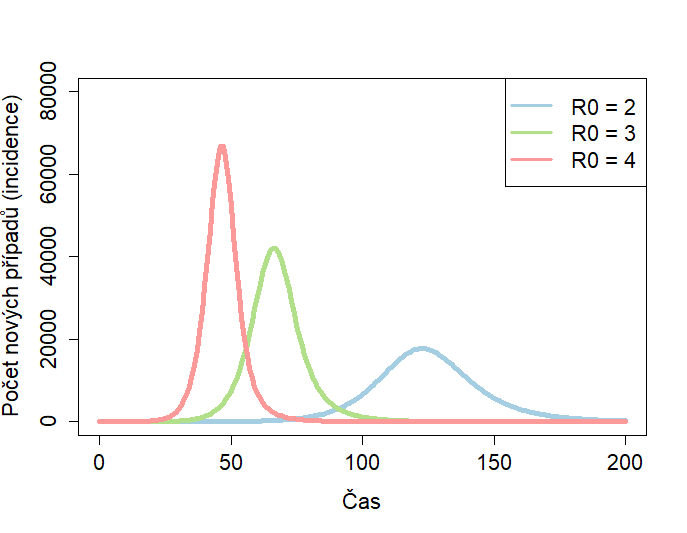
\includegraphics[width=0.99\textwidth]{pic/figsir2.png}
	\end{minipage}
\end{center}
\caption{Dynamika SIR modelu (\ref{SIR1}). Levý panel: typické numerické řešení modelu; $N=1000000$, $\beta=0.4$, $\gamma=0.1$. Pravý panel: závislost časového vývoje počtu nových případů (incidence) na základním reprodukčním čísle $R_0$; $N=1000000$, $\gamma=0.1$, $\beta=\gamma R_0$.}
\label{kendrick1}
\end{figure}

%\subsection*{Matematické modelování infekčních nemocí}

\paragraph{Matematické modelování infekčních nemocí:} Pravé neštovice, malárie a nyní covid-19 nejsou jedinými infekčními nemocemi, pro něž byly vytvořeny matematické modely. Naopak, téměř jakákoli infekční nemoc, na kterou si můžeme vzpomenout, už pravděpodobně byla více či méně modelována \cite{AndersonMay1991,KeelingRohani2008,VynnyckyWhite2010,Ronn_etal2017,Finger_etal2019}. Nejčastěji šlo o HIV, chřipku, malárii a další komáry přenášené infekce, spalničky a další dětské nemoci, po roce 2014 pak o ebolu (obr.\,\ref{wos}). Epidemické modely, popisující ze své podstaty přenos nějaké entity při kontaktu a schopnost tuto entitu po nějakou dobu přenášet dále, se využívají také při studiu situací přesahujících oblast epidemiologie, jako je problém šíření počítačových virů \cite{YangYang2014}, zombiismu \cite{Alemi_etal2015}, fám či dohadů \cite{DaleyKendall1964}.

\begin{figure}[h]
\begin{center}
	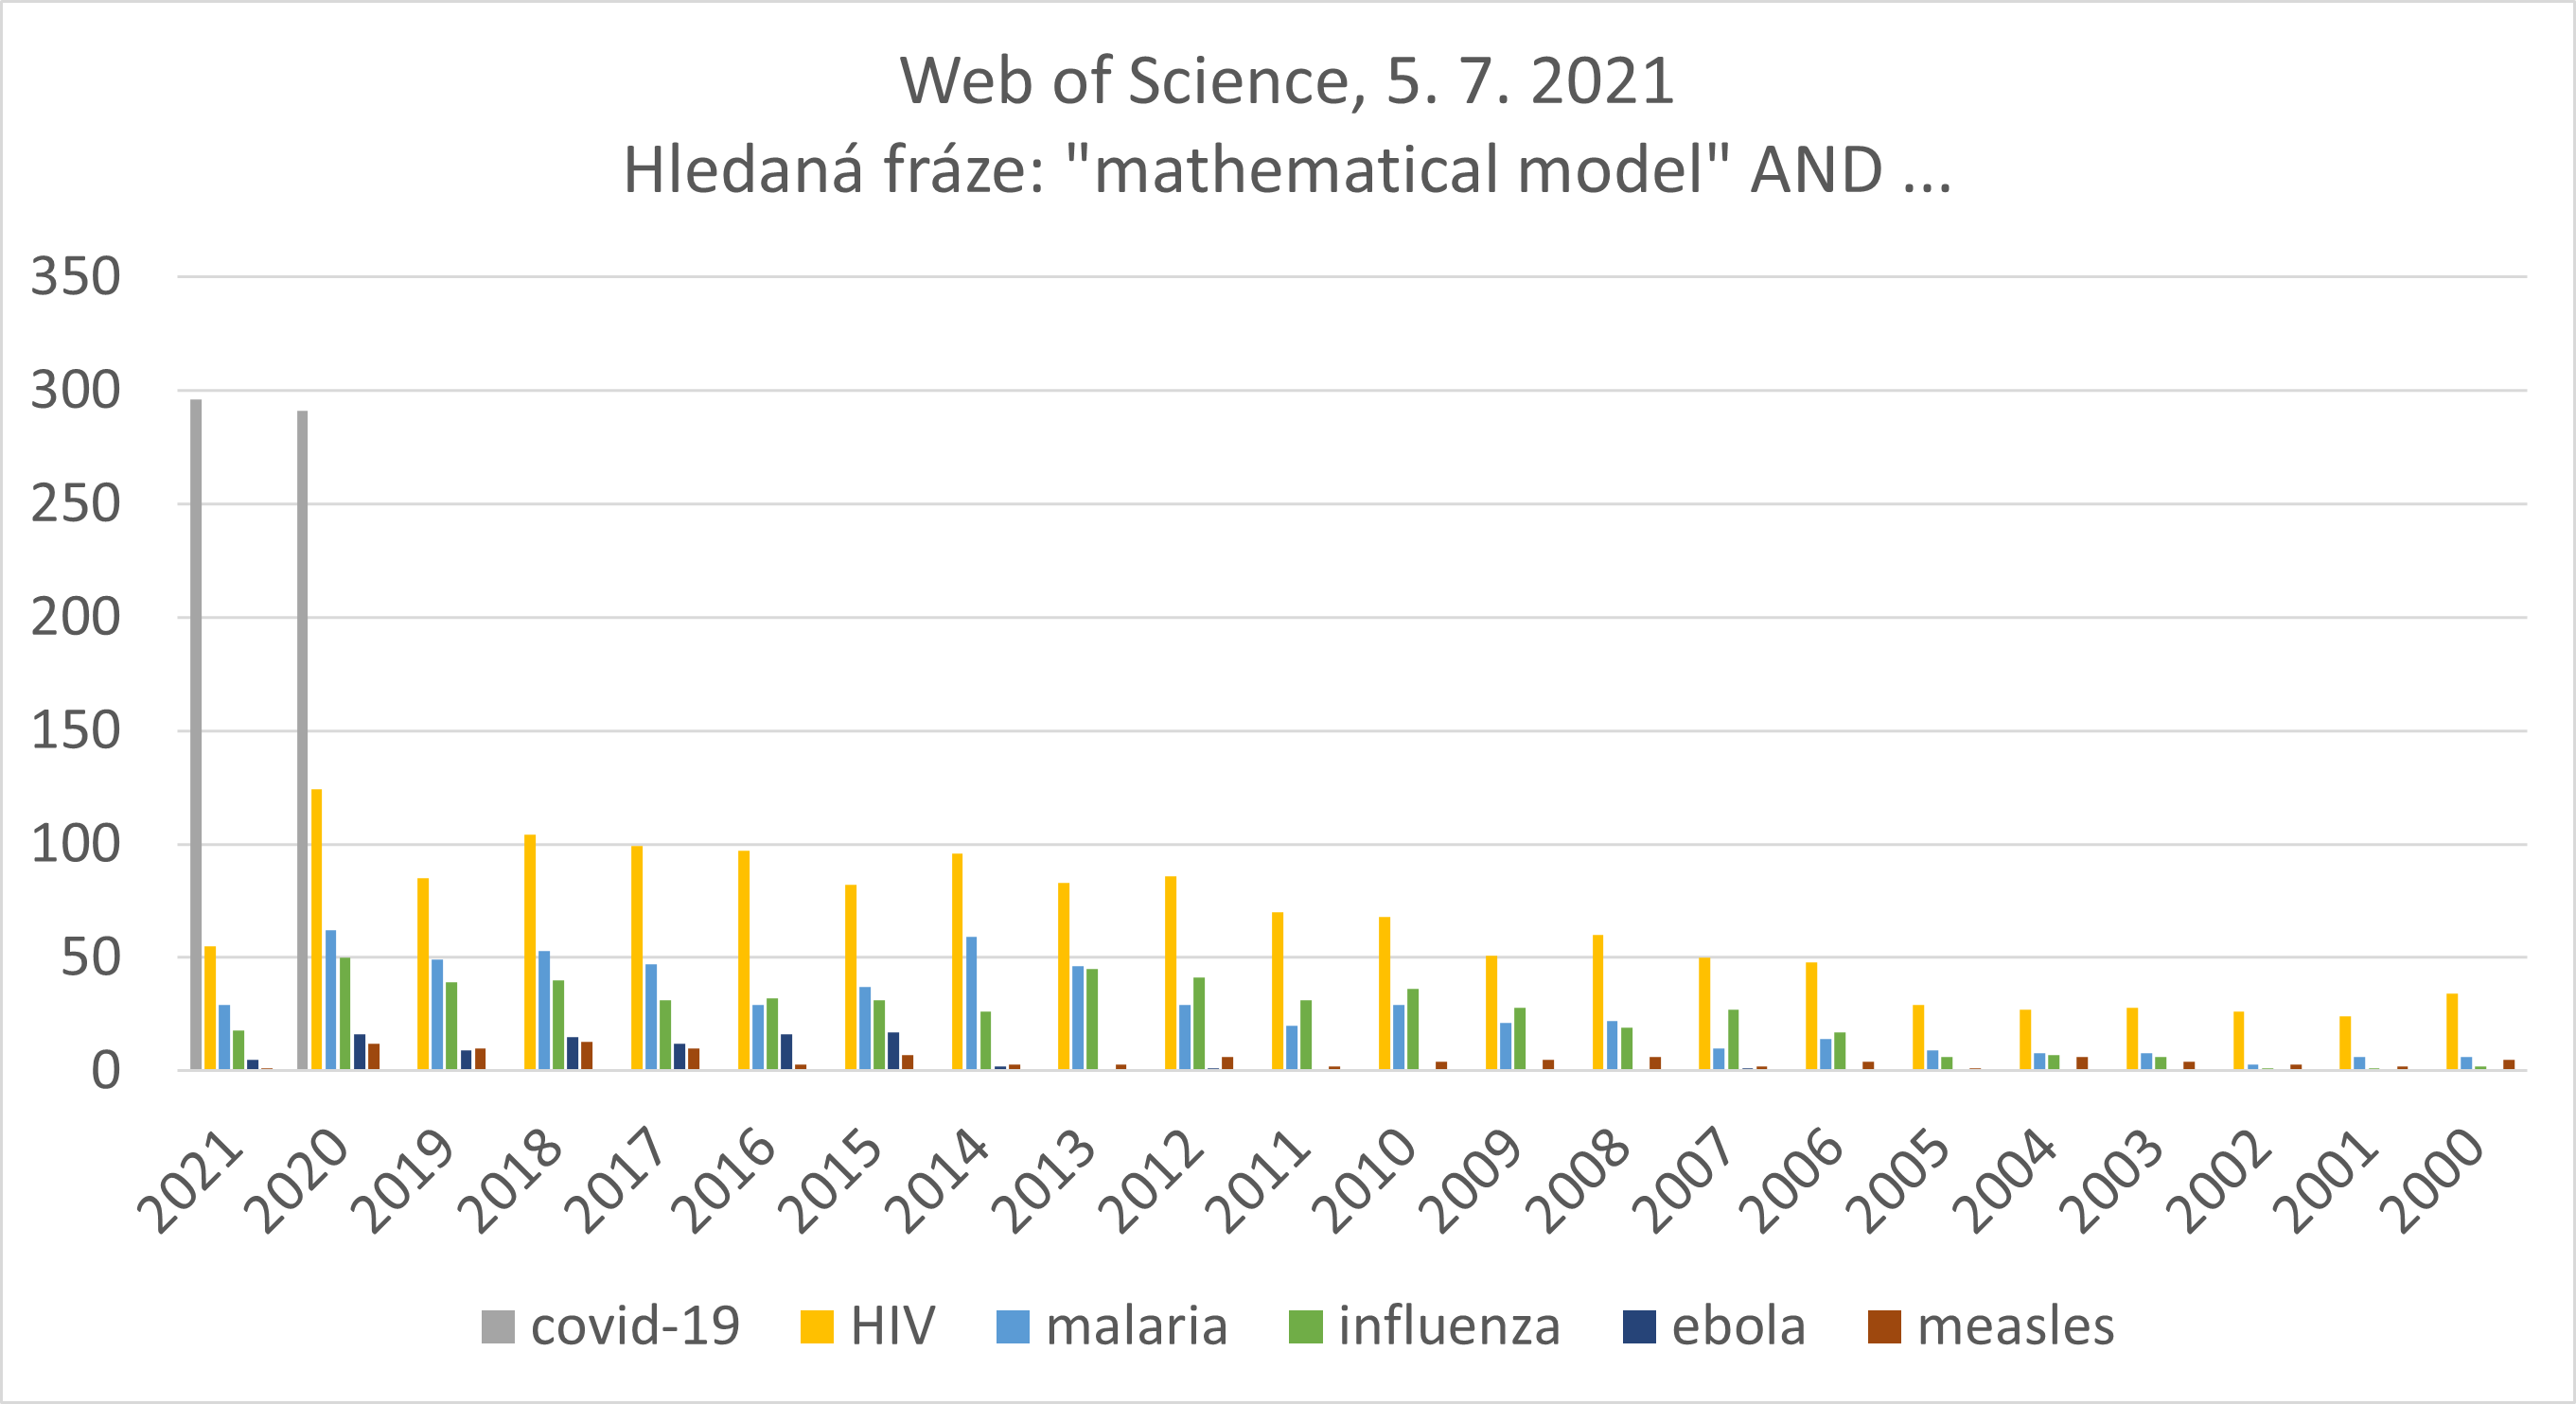
\includegraphics[width=0.85\textwidth]{pic/wos_papers.png}
\end{center}
\caption{Počet vědeckých článků s tematikou matematického modelování infekčních nemocí v časopisech indexovaných portálem Web of Science. Kromě toho k 5.\,7.\,2021 vrátil preprintový server medRxiv 10 844 článků v reakci na frázi „mathematical model“ AND covid-19.}
\label{wos}
\end{figure}

\section*{Matematické modelování reálných epidemií}

Zatímco matematika epidemií je relativně jednoduchá, problémy nastávají, setká-li se s reálným světem. Modely jsou z principu nedokonalé, mnohdy založené na řadě netestovatelných, nepřesných, či dokonce úmyslně nepřesných předpokladů (například standardní předpoklad dokonalého míchání populace), data jsou neúplná či nepřesná. Jde-li navíc o rozsáhlou epidemii, či dokonce pandemii, jako v případě covid-19, vstupují do hry další faktory, např. v zásadě kontinuální proměna situace (změny v chování lidí, nové informace o infekci, nové postupy v boji s epidemií), tlak veřejnosti (jak bychom měli ideálně reagovat, bude dané opatření dostatečně fungovat, jak se bude epidemie dále vyvíjet), či dokonce vlastní obavy (co když jsme někde udělali chybu, co když to s doporučeními přeženeme, nebo naopak budeme příliš optimističtí). Řečeno s lehkou nadsázkou, je to, jako když stavíme koleje, přičemž za zády už slyšíme přijíždět vlak. 

Jedna z takových kontinuálních proměn se týkala základní struktury samotných modelů. Jak postupně přicházely nové informace, modelová struktura se vyvíjela. Počáteční SIR model jako základ pro výpočet bazálních parametrů epidemie zmíněných výše se brzy změnil na SEIR model s třídou $E$ popisující nakažené, ale zatím neinfekční jedince. Z tohoto modelu se následně stal SEIAR model s třídou $A$ jedinců asymptomatických po celou dobu epidemie, a nakonec SEPIAR model, kdy se třída $I$ rozdělila na třidu $P$ presymptomatických jedinců (infekční, zatím bez symptomů) a následnou třídu $I$ jedinců se symptomy (obr.\,\ref{SEPIAR1}). Zahrnutí tříd $A$ a $P$ bylo důležité z toho důvodu, že zatímco jedinci asymptomatičtí po celou dobu své infekčnosti mají nižší nakažlivost, symptomatičtí infekční jedinci mají díky (samo)izolaci nižší množství kontaktů. Řízení epidemie prostřednictvím opatření, ale také vlastní změny chování vedou k časově proměnné hodnotě parametru $\beta$ modelu (\ref{SIR1}); tento parametr se však vyskytuje ve všech uvedených modelových variantách. V důsledku změn tohoto parametru také epidemie covid-19 nikde neodpovídá pouze jedné vlně. V České republice jsme byli svědky už čtyř epidemických vln. Kromě toho se v čase měnila také prodleva mezi testem a reportingem v případě infekčnosti, účinnost trasování a nemocniční péče, ochota plošná opatření dodržovat, převládající virová varianta či intenzita očkování. Epidemie covid-19 je tak nejen epidemiologický, ale do značné míry také sociální fenomén.   

\begin{figure}[h]
	\begin{center}
		\begin{tikzpicture}[->,>=stealth',shorten >=1pt,auto,node distance=2.5cm, semithick]
			\tikzstyle{every state}=[fill=white,draw=black,text=black]
			\node[state] 	(A) {$S$};
			\node[state]    (B) [right of=A] {$E$};
			\path (A) edge [line width=0.5mm] node {} (B);
			\node[state]    (C) [right of=B] {$P$};
			\path (B) edge [line width=0.5mm] node {} (C);
			\node[state]    (I) [above of=C] {$A$};
			\path (B) edge [line width=0.5mm] node {} (I);
			\node[state]    (S) [right of=C] {$I$};
			\path (C) edge [line width=0.5mm] node {} (S);
			\node[state]    (Z) [right of=S] {$R$};
			\path (S) edge [line width=0.5mm] node {} (Z);
			%\node[state]    (D) [above of=C] {$I_R$};
			%\path (C) edge [line width=0.5mm] node {} (D);
			\path (I) edge [line width=0.5mm] node {} (Z);
			%\node[state]    (R) [above of=D] {$R$};
			%\path (D) edge node {} (R) 
			%(I) edge node {} (R)
			%(D) edge node {} (R)
			%(Z) edge [right] node {} (R);
			%(S) edge node {$\gamma_I$} (R);
			%\node[state]    (D) [rectangle, right of=S, color=blue, text=white] {$H$};
			%\path (S) edge node {} (D);
		\end{tikzpicture}
	\end{center}
	\caption{Schéma SEPIAR modelu. Jednotlivé třídy, nebo také říkáme kompartmenty: $S$ -- vnímaví jedinci, $E$ -- nakažení, ale zatím neinfekční jedinci, $P$ -- jedinci zatím bez symptomů, ale už nakažliví (presymptomatiční), $I$ -- symptomatičtí infekční jedinci, $A$ -- jedinci bez symptomů po celou dobu své infekce (asymptomatiční), $R$ -- uzdravení (případně zemřelí) jedinci.}
	\label{SEPIAR1}
\end{figure}

%\subsection*{Základní zákon epidemie}

\paragraph{Základní zákon epidemie:} Výrazu $\beta\,I[t]/N$ v první rovnici modelu (\ref{SIR1}) a podobnému výrazu v dalších modelech se říká \emph{síla infekce}. Síla infekce vyjadřuje rychlost, s jakou se vnímaví jedinci v populaci infikují, nebo též pravděpodobnost, že se během časové jednotky určitý vnímavý jedinec nakazí. Zkusme tuto pravděpodobnost více rozepsat. Nechť vnímavý jedinec potká za jednotku času v průměru $c$ jiných lidí. Pokud jsou tyto kontakty v rámci populace náhodné, případně pokud je infekce v populaci náhodně rozšířená, je $I[t]/N$ pravděpodobnost, že náhodně vybraný jedinec je v čase $t$ infekční, a tedy $c\,I[t]/N$ je počet infekčních jedinců, které za jednotku času vnímavý jedinec potká (nebo též rychlost, s jakou infekční jedince potkává). Nechť je dále $b$ pravděpodobnost, že se vnímavý jedinec při jednom každém z těchto kontaktů nakazí. Pak pravděpodobnost, že se vnímavý jedinec během jednotky času nakazí, je 
\begin{equation}
(1-(1-b))^{c\,I[t]/N} \approx b\, c \, \frac{I[t]}{N}.
\end{equation}
Rozlišujeme dva druhy nefarmaceutických protiepidemických opatření, opatření určená k omezení kontaktů (zavření škol či restaurací, omezení pohybu, apod.) a osobní ochranná opatření omezující pravděpodobnost nákazy při kontaktu (roušky, ruce, rozestupy, užívání vitamínů apod.). Zatímco první typ opatření snižuje hodnotu $c$, druhý typ omezuje pravděpodobnost nákazy při kontaktu a snižuje hodnotu $b$. Označíme-li proporcionální redukci parametru $b$ jako $r_b$ a parametru $c$ jako $r_c$, pak složený parametr $\beta$ v~modelu (\ref{SIR1}) nebo v jakémkoli příbuzném modelu můžeme rozepsat jako $\beta = r_b\,b\,r_c\,c$. Zatímco hodnotu $c$ můžeme odhadnout z výsledků dotazníkových šetření a je mimo jiné dostupná v literatuře \cite{Prem_etal2017}, hodnotu $r_c$ můžeme odhadnout taktéž z výsledků dotazníkových šetření. V Česku to můžeme udělat s využitím projektu „Život během pandemie“ agentury PAQ Research \cite[\url{www.zivotbehempandemie.cz}]{paqcovid}. Odhad hodnot $b$ a $r_b$ je komplikovanější, v zásadě jej můžeme získat pouze prostřednictvím \emph{kalibrace modelu}, kdy se určitou systematickou změnou hodnot těchto parametrů snažíme dosáhnout toho, aby vypočtený průběh epidemie odpovídal co nejvíce reálným pozorováním \cite{Yang_etal2014,King_etal2016}. 

Podobně jako v SIR modelu je i v jeho příbuzných SEIR, SEIAR a SEPIAR modelech (efektivní) reprodukční číslo $R$ násobkem parametru $\beta$. Opatření znamenající snížení hodnoty $\beta$ tak implikují snížení exponenciálního růstu a v případě poklesu reprodukčního čísla $R$ pod hodnotu jedna dokonce jeho úplné potlačení. Nepochopení síly exponenciálního růstu však přináší velké riziko. Dlouho se totiž relativně nic neděje, až najednou začnou čísla letět prudce vzhůru. Pak už je však těžké zatáhnout za záchrannou brzdu, zvláště má-li infekce latentní periodu a mnoho nakažených čeká za oponou na chvíli, kdy se stanou nakažlivými. Rychlé zavedení přísných opatření naopak vyvolává všeobecný nesouhlas, neboť případů je v dané chvíli relativně málo. V Austrálii například opakovaně zaváděli přísná opatření i při objevení se jen několika málo případů covid-19 \cite{australia_opatreni}. Je to poněkud extrémní případ, nicméně i toto zdánlivě nesmyslné rozhodnutí dává ve světle znalosti základního zákona epidemie a exponenciálního růstu smysl. Opatření se tak nezavádějí kvůli jednotkám až desítkám případů, ale proto, abychom předešli desítkám a stovkám tisíc případů. Znalost dynamiky epidemie, založená na matematických modelech a známá více než 100 let, je zásadní při jakémkoli praktickém rozhodování.

Uveďme si příklad. Uvažujme SEIR model
\begin{equation}
	\begin{array}{l}
		\displaystyle{S[t+1] = S[t] - b\,r_c\,c \, \frac{S[t]\,I[t]}{N}}, \\[3ex]
		\displaystyle{E[t+1] = E[t] + b\,r_c\,c \, \frac{S[t]\,I[t]}{N} - \sigma E[t]}, \\[3ex]
		\displaystyle{I[t+1] = I[t] + \sigma E[t] - \gamma I[t]}, \\[3ex]
		\displaystyle{R[t+1] = R[t] + \gamma I[t]},
	\end{array}
	\label{SEIR1}
\end{equation}
kde $E$ je třída jedinců, kteří už jsou nakažení, ale stále ještě ne infekční (délku odpovídající latentní periody infekce odráží parametr $\sigma$). Zaveďme nyní od určitého okamžiku po vypuknutí epidemie opatření, která sníží počet denních kontaktů o 65 \% (tedy $r_c$, do té doby rovno jedné, bude nyní $0.35$), a v určitém čase pak tato opatření opět zrušme ($r_c$ se vrátí na hodnotu 1). Výsledkem je druhá vlna epidemie, jak jsme několikrát pozorovali i v realitě (obr.\,\ref{SEIR-vlna}). Důvodem vzniku nové vlny je, že po rozvolnění se hodnota efektivního reprodukčního čísla $R$ opět vrátí nad hodnotu 1, neboť je v populaci stále dostatek vnímavých jedinců (tedy velký poměr $S[t]/N$), a tedy kontakty mezi vnímavými a infekčními jedinci jsou stále dostatečně časté.

\begin{figure}[h]
	\begin{center}
		%\begin{minipage}[m]{0.45\linewidth}
			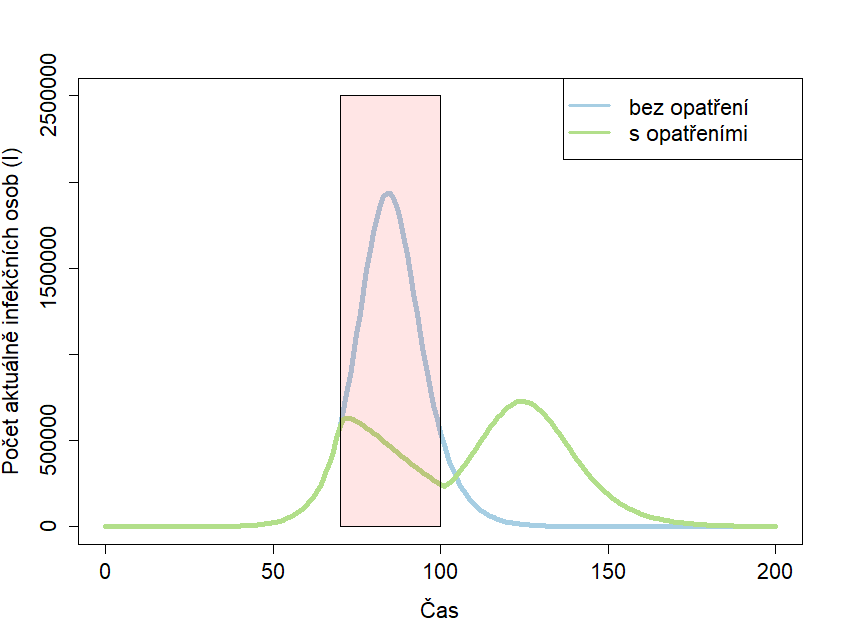
\includegraphics[width=0.6\textwidth]{pic/two_waves.png}
		%\end{minipage}
		%\hspace{2ex}
		%\begin{minipage}[m]{0.45\linewidth}
		%	\includegraphics[width=0.9\textwidth]{spanish_flu.png}
		%\end{minipage}
	\end{center}
	\caption{Dynamika SEIR modelu (\ref{SEIR1}) v případě zavedení nefarmaceutických opatření snižujících kontakty a vznik druhé vlny epidemie v případě jejich brzkého zrušení; $N=10000$, $c=10$, $R_0=3$, $\gamma=1/7$, $b=R_0\,\gamma/c$, $\sigma=1/3$; červený panel označuje období působení opatření, kdy byl počet denních kontaktů $c$ snížen o 65 \% (tedy $r_c=0.35$); osobní protektivní opatření zde pro jednoduchost neuvažujeme čili volíme $r_b=1$. %Pravý panel: šíření viru španělské chřipky se v řadě amerických měst obnovilo poté, co se brzy upustilo od přijatých opatření; převzato z \cite{Hatchett_etal2007}. Kontakty mezi nemocnými a vnímavými jedinci byly stále dostatečně časté.
	}
	\label{SEIR-vlna}
\end{figure}

\section*{covid-19: data a modely}

Už jsme mluvili o tom, jak se díky novým znalostem měnila představa o epidemiologické struktuře infekce: od původního SIR modelu, archetypu epidemického modelu, až k SEPIAR modelu se čtyřmi typy infikovaných jedinců. Průběh epidemie je také prostorově rozrůzněný (stačí se podívat na mapu okresů a dynamiky nemocných v nich), věkově rozrůzněný (mortalita roste s věkem, účinnost vakcinace s věkem klesá, s věkem se také mění pravděpodobnost, že jedinci budou mít symptomy, či pravděpodobnost, že symptomatičtí jedinci budou mít těžší průběh a vyžadovat hospitalizaci), a rozrůzněný vzhledem ke struktuře kontaktů (kontakty ve škole, doma, v práci či jinde). Populace je také heterogenní z hlediska individuálního počtu kontaktů: mnoho z nás má během dne relativně málo kontaktů, avšak někteří z nás, tzv.\ superpřenašeči, jich mají mnoho. 

Při konstrukci jakéhokoli epidemického modelu, zvláště pokud má popsat řadu po sobě jdoucích epidemických vln, bychom všechny tyto aspekty měli zvážit. Různé typy modelů umožňují různé aspekty různě efektivně zahrnout. Měli bychom si proto předem říci, co je cílem modelu. Kromě toho si musíme být vědomi dat, jaká máme k dispozici. Na základě toho si pak stanovíme typ a strukturu modelu. Model obsahuje mnoho parametrů, které je třeba určit. Můžeme je rozdělit do dvou skupin: parametry, které odhadneme z jiných dat než z časových průběhů počtu jedinců v jednotlivých třídách, a parametry určené kalibrací modelu, tedy jejich určitým systematickým nastavováním tak, aby dynamika modelu odpovídala pozorované dynamice epidemie. Nakonec je třeba posoudit predikční schopnosti modelu, nejlépe s využitím dat, která nebyla použita k jeho konstrukci. Je-li shoda modelové a skutečné dynamiky epidemie dostatečná, model je tzv.\ validovaný. Nyní je čas definovat různé možné scénáře budoucího vývoje (např.\ možné strategie rozvolňování či různé předpokládané rychlosti dodávek vakcín) a vypočítat možné budoucí chování epidemie. Ideálně jsou pak takové modelové projekce doprovázeny nějakou kvantifikovatelnou mírou nejistoty.

Z hlediska typu modelu rozlišujeme dvě hlavní kategorie: kompartmentové modely a agentově orientované modely. Kompartmentové modely dělí společnost na konečný počet tříd, kompartmentů. V každém z těchto kompartmentů považujeme jedince epidemiologicky i z hlediska chování za homogenní. SIR model (\ref{SIR1}) tak dělí populaci do tří kompartmentů a SEIR model (\ref{SEIR1}) do čtyř. Pokud bychom však uvažovali SEPIAR model z obr.\,\ref{SEPIAR1} v každém z 206 katastrů obcí s rozšířenou působností a populaci navíc rozdělili do tří věkových skupin (například děti do 19 let, střední věková třída 20--64 let a senioři 65 a více let), měl by náš model $6 \times 206 \times 3 = 3708$ kompartmentů, propojených epidemickými procesy a mobilitou. Další možné kompartmenty snadno vymyslíme: hospitalizovaní jedinci, jedinci na JIP, jedinci s různým stupněm rizikovosti (lidé s malým a velkým počtem kontaktů, rouškaři versus antirouškaři), různé fáze procesu vakcinace s různou účinností vakcíny apod. Agentově orientované modely jsou naopak charakteristické tím, že explicitně reprezentují a sledují události pro každého jedince zvlášť \cite{Smith_etal2018}. Každý jedinec tak může mít unikátní atributy, stanovené na základě pravděpodobnostních distribucí určitých veličin (např.\ velikost domácnosti či počet přátel), ale také na základě vztahu k epidemii (např.\ vytrasován a v izolaci či naočkován první dávkou). Můžeme také pracovat s různou délkou různých typů kontaktů a také se specifickými pravděpodobnostmi přenosu infekce při takových kontaktech. V neposlední řadě máme pod kontrolou časovou dynamiku kontaktní struktury a snadno tak modelujeme v principu individuální procesy, jako jsou karanténa či trasování, tedy procesy, které v kompartmentových modelech můžeme modelovat jen velmi hrubě. Agentově orientované modely, které jsme v rámci centra BISOP v průběhu pandemie covid-19 vytvořili a využívali, si představíme v kapitolách \ref{Skoly} a \ref{Agentni_modely}.  

\section*{První vlna epidemie covid-19 v Česku}

Jednou z nejčastějších otázek provázejících epidemii covid-19 nejen v Česku bylo, jaká opatření fungují a do jaké míry. Je to naprosto přirozená a pochopitelná otázka, ale odpověď na ni je velmi nesnadná. Statistické studie publikované na toto téma naznačují, že mezi nejúčinnější opatření patří zákaz shromažďování, omezení pohybu či zavření škol, a shodují se v tom, že potlačení epidemie je možné jen vhodnou kombinací různých opatření \cite{Flaxman_etal2020,Li_etal2020,Haug_etal2020,Liu_etal2021}. Určitým problémem dat vstupujících do těchto analýz je, že opatření byla často aplikována či rušena skupinově, nikoli individuálně, a v mnoha případech následují v určitém stejném pořadí. Výše uvedené studie to z pochopitelných důvodů řeší tak, že do svých analýz zahrnují průběhy zavádění a rušení opatření v mnoha zemích světa, a tím pořadí a současnost různých opatření do jisté míry desynchronizují. V řadě zemí včetně Česka se například zavřely školy nějakou dobu předtím, než se zavedly roušky. Jak by to dopadlo, kdyby se školy zavřely týden či dva po zavedení roušek? I když by bylo velmi zajímavé v jednom kraji zavřít školy, v jiném hospody, ve třetím obchody a ve čtvrtém zábavu a sledovat a analyzovat jejich vývoj, v době epidemie na experimenty není čas.

\begin{table}[h]
	\begin{center}
	\begin{tabular}{lp{8cm}}
		\hline\noalign{\smallskip}
		Datum & Opatření \\
		\noalign{\smallskip}\hline\noalign{\smallskip}
		11. 3. 2020 & Zavřeny školy, doporučena práce z domova \\
		12. 3. 2020 & Omezení cestování \\
		14. 3. 2020 & Zavření restaurací, sportovních a kulturních zařízení a většiny obchodů \\ 
		19. 3. 2020 & Nutnost nosit na veřejnosti roušky, dodržovat rozestupy a používat dezinfekci \\
		\noalign{\smallskip}\hline
	\end{tabular}
	\end{center}
	\caption{Plošná opatření proti epidemii covid-19 v Česku v průběhu první vlny na jaře 2020.}
	\label{table:interventions}
\end{table}

Pomoci mohou standardní epidemické modely typu SIR či SEPIAR, strukturované podle typu kontaktů a umožňující jednotlivá opatření kdykoli zapínat a vypínat. Zatímco v detailních agentově orientovaných modelech to můžeme dělat velmi sofistikovaně (viz kapitoly \ref{Skoly} a \ref{Agentni_modely}), v kompartmentových modelech jsme v zásadě odkázáni na časový vývoj počtu kontaktů a hypotézy o tom, do jaké míry daná opatření počty daných typů kontaktů redukují. Alternativně se můžeme ptát, jaká redukce různých typů kontaktů je dostatečná pro to, aby epidemie přestala růst.   

Jedním z modelů, které jsme v rámci centra BISOP vytvořili, je model první epidemické vlny z jara 2020. Detaily modelu je možné najít v práci \cite{Berec_modelB}, zde popíšeme jen jeho základní strukturu. Jde o kompartmentový SEPIAR model, v němž se navíc část symptomatických infekčních jedinců rozhodne netestovat, tudíž se neobjeví v oficiálních statistikách. Model je věkově i prostorově rozlišený a je kalibrovaný na časový vývoj kumulativního počtu detekovaných (v té době dominantně symptomatických) jedinců, rozlišený podle věku (levý sloupec v obr.\,\ref{shelterning_seniors}). Tento model pokrývá období od začátku epidemie do 7.\,5.\,2020, kdy po celou dobu v zásadě platila stejná protiepidemická opatření, a pro které jsme měli k dispozici průměrnou hodnotu pohledu kontaktů ve školách, práci, domácnostech a jinde. Model také explicitně zahrnuje načasování zavedení jednotlivých opatření (tab.\,\ref{table:interventions}). S takto nastaveným modelem jsme zkoumali různé alternativní scénáře, které v daném období mohly nastat. Ukážeme si tři z nich. První scénář uvažuje zahájení všech přijatých opatření o čtyři dny dříve či čtyři dny později než ve skutečnosti. Jak ukazuje obr.\,\ref{scenariosR1R2}, každé čtyři dny zpoždění znamenaly zdvojnásobení počtu detekovaných symptomatických infekčních jedinců ke konci zkoumaného období. Mimo jiné tento výsledek jasně demonstruje důsledky exponenciálního růstu: včasný zásah je zásadní. 

\begin{figure}
	\begin{center}
		\begin{minipage}[m]{0.45\textwidth}
			A) \\
			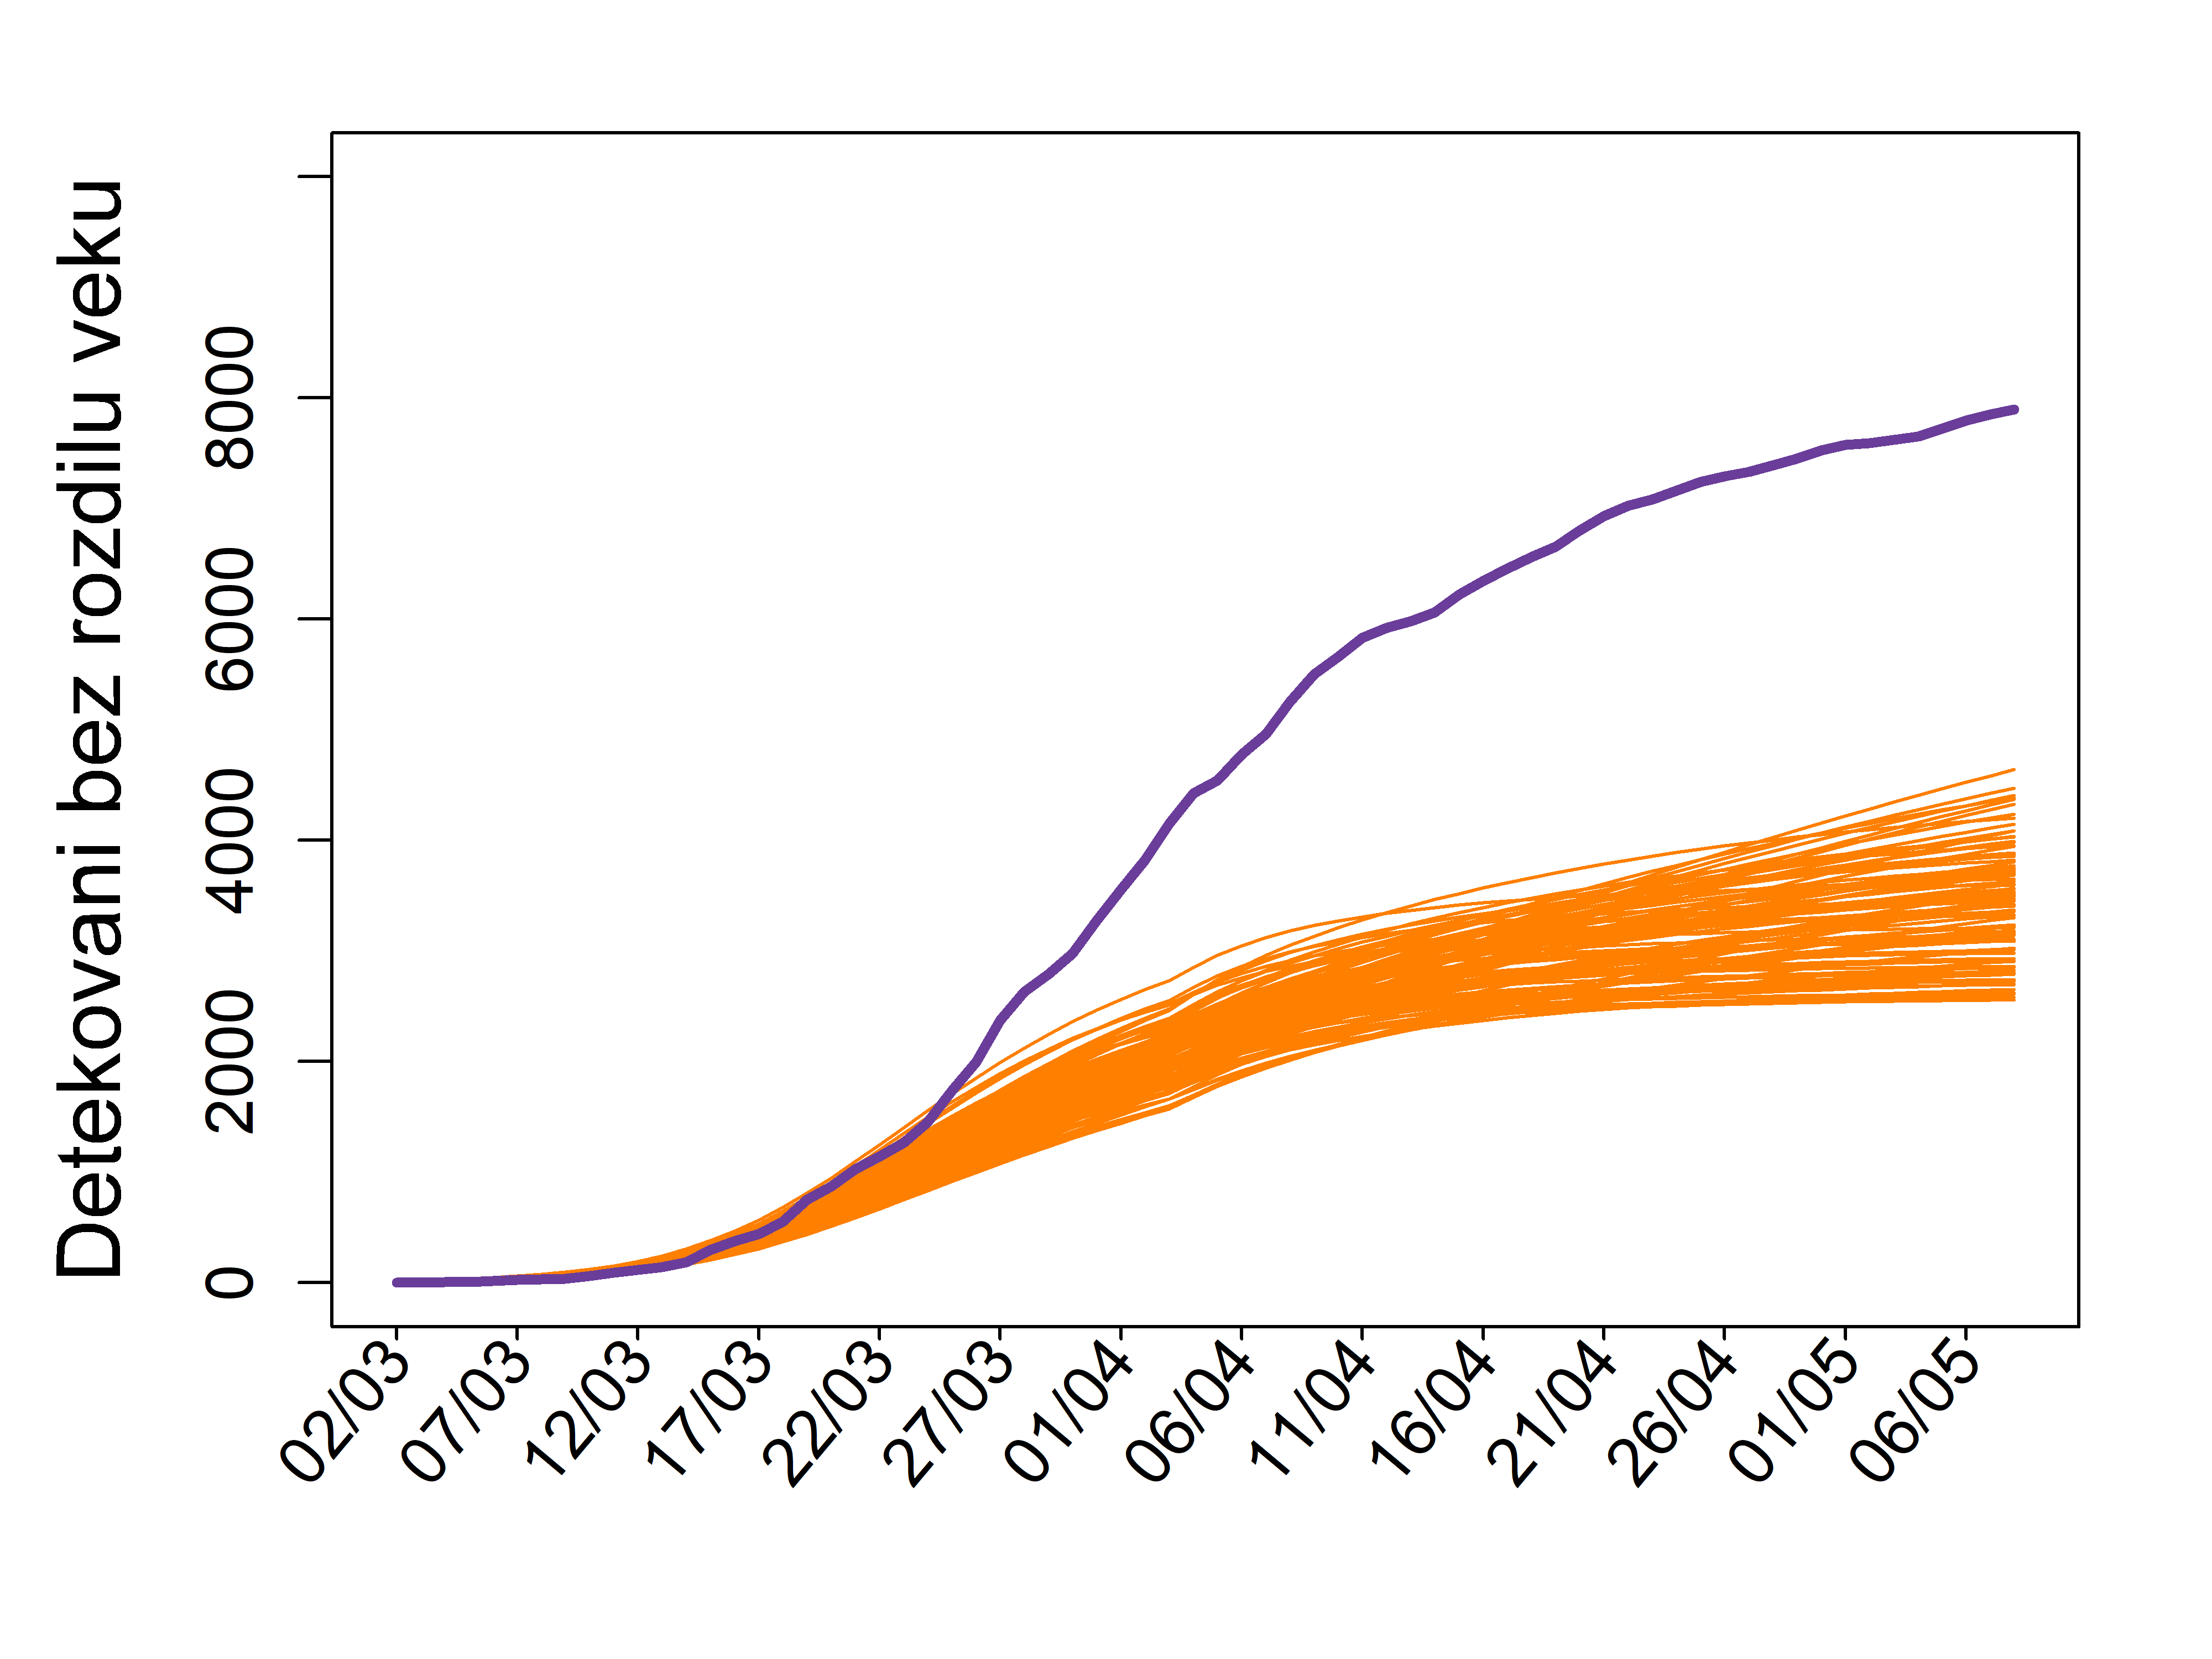
\includegraphics[width = \textwidth]{pic/sc_4earlier.png}
		\end{minipage}
		\begin{minipage}[m]{0.45\textwidth}
			B) \\
			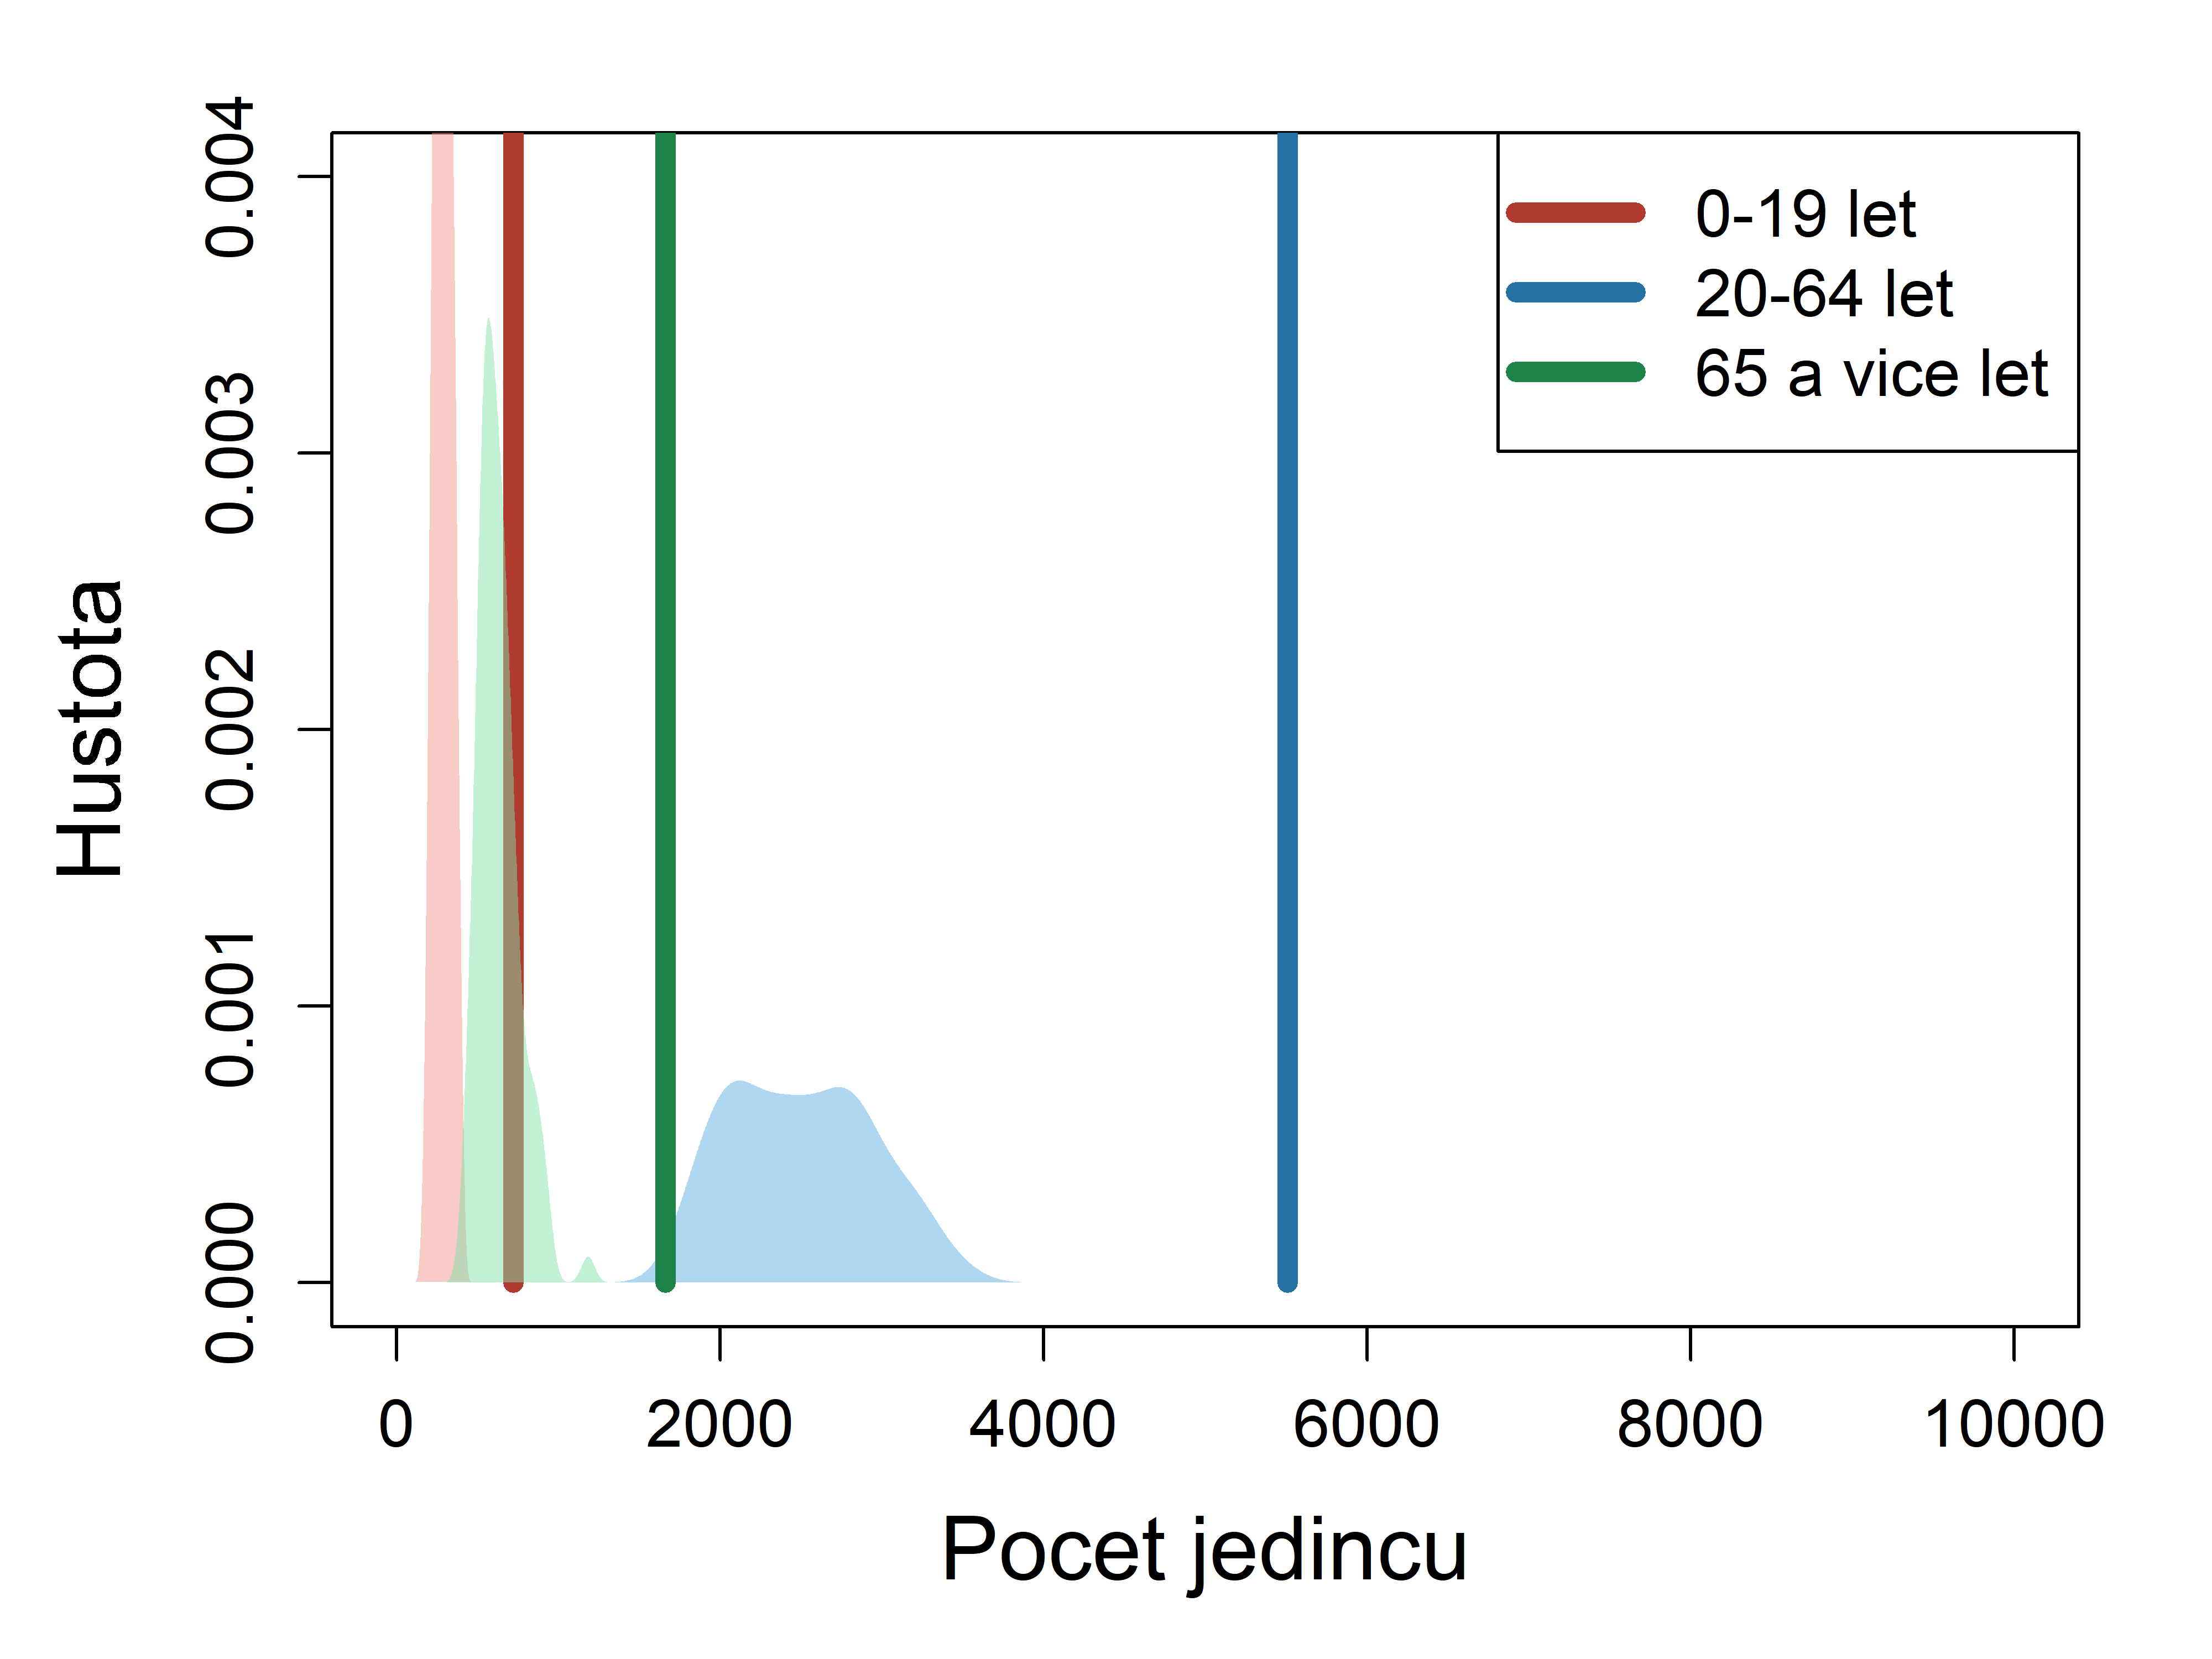
\includegraphics[width = \textwidth]{pic/sc_4earlier_PDF.png}
		\end{minipage} \\[1ex]
		\begin{minipage}[m]{0.45\textwidth}
			C) \\
			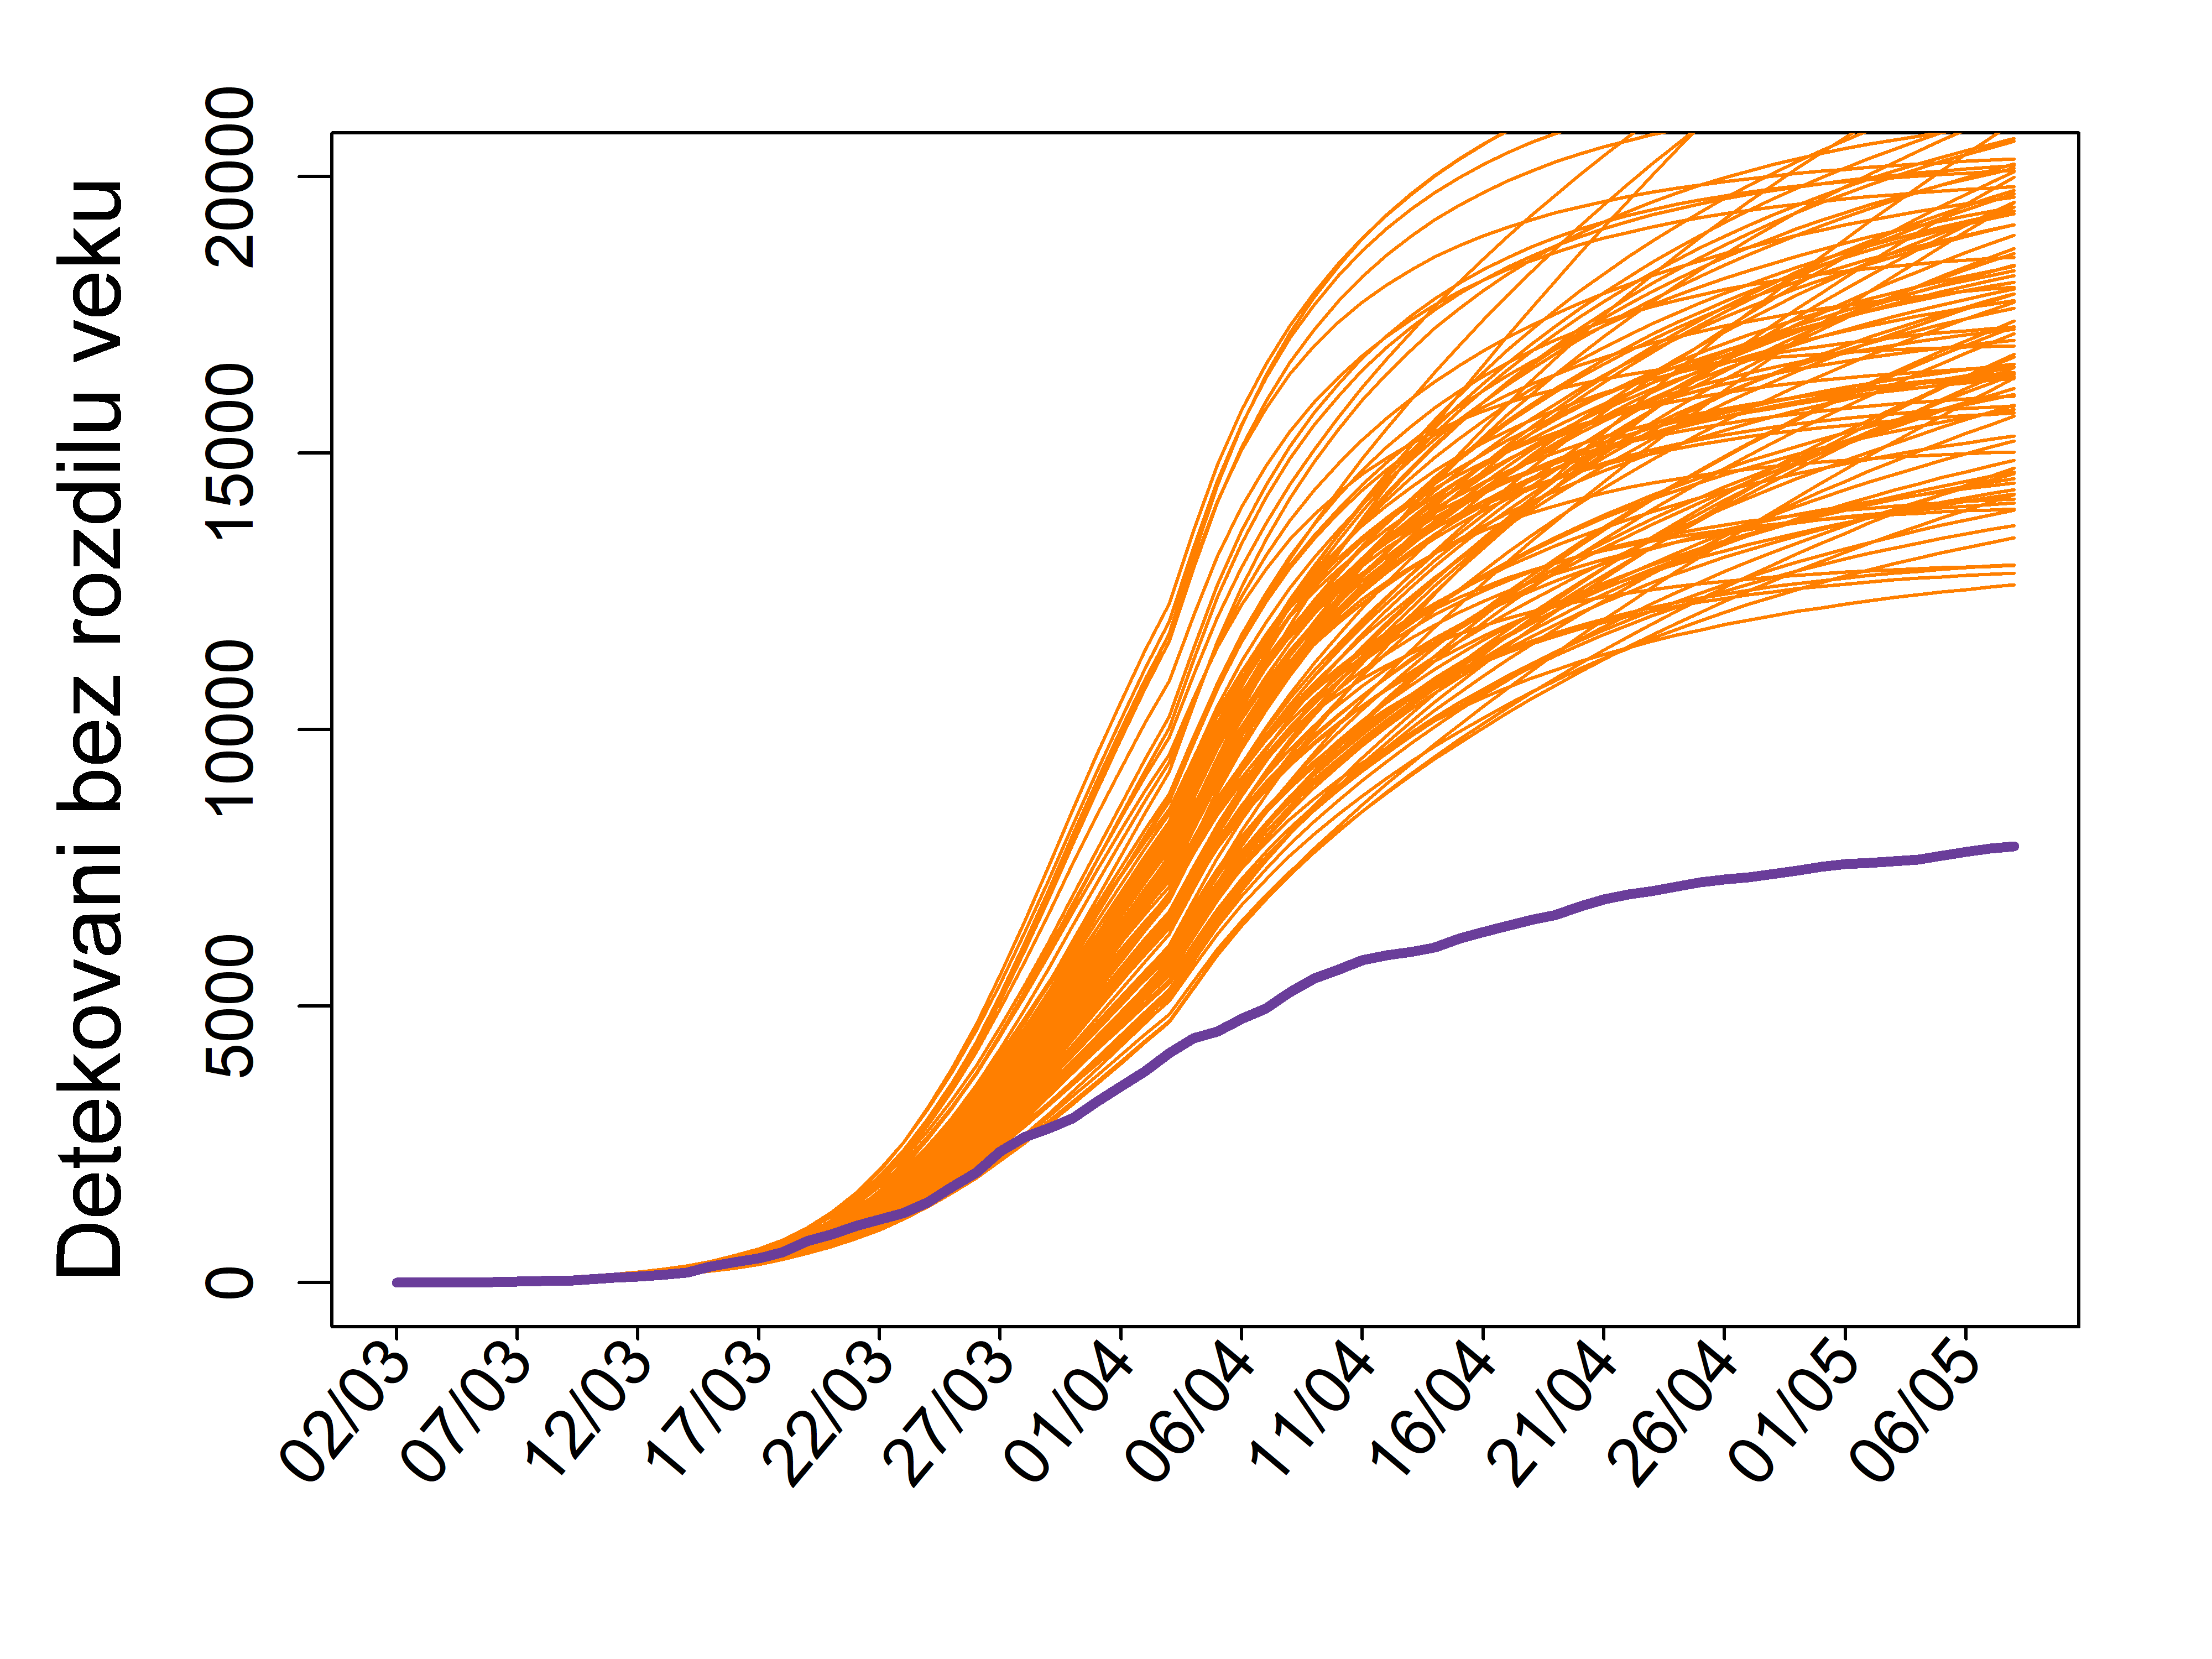
\includegraphics[width = \textwidth]{pic/sc_4later.png}
		\end{minipage}
		\begin{minipage}[m]{0.45\textwidth}
			D) \\
			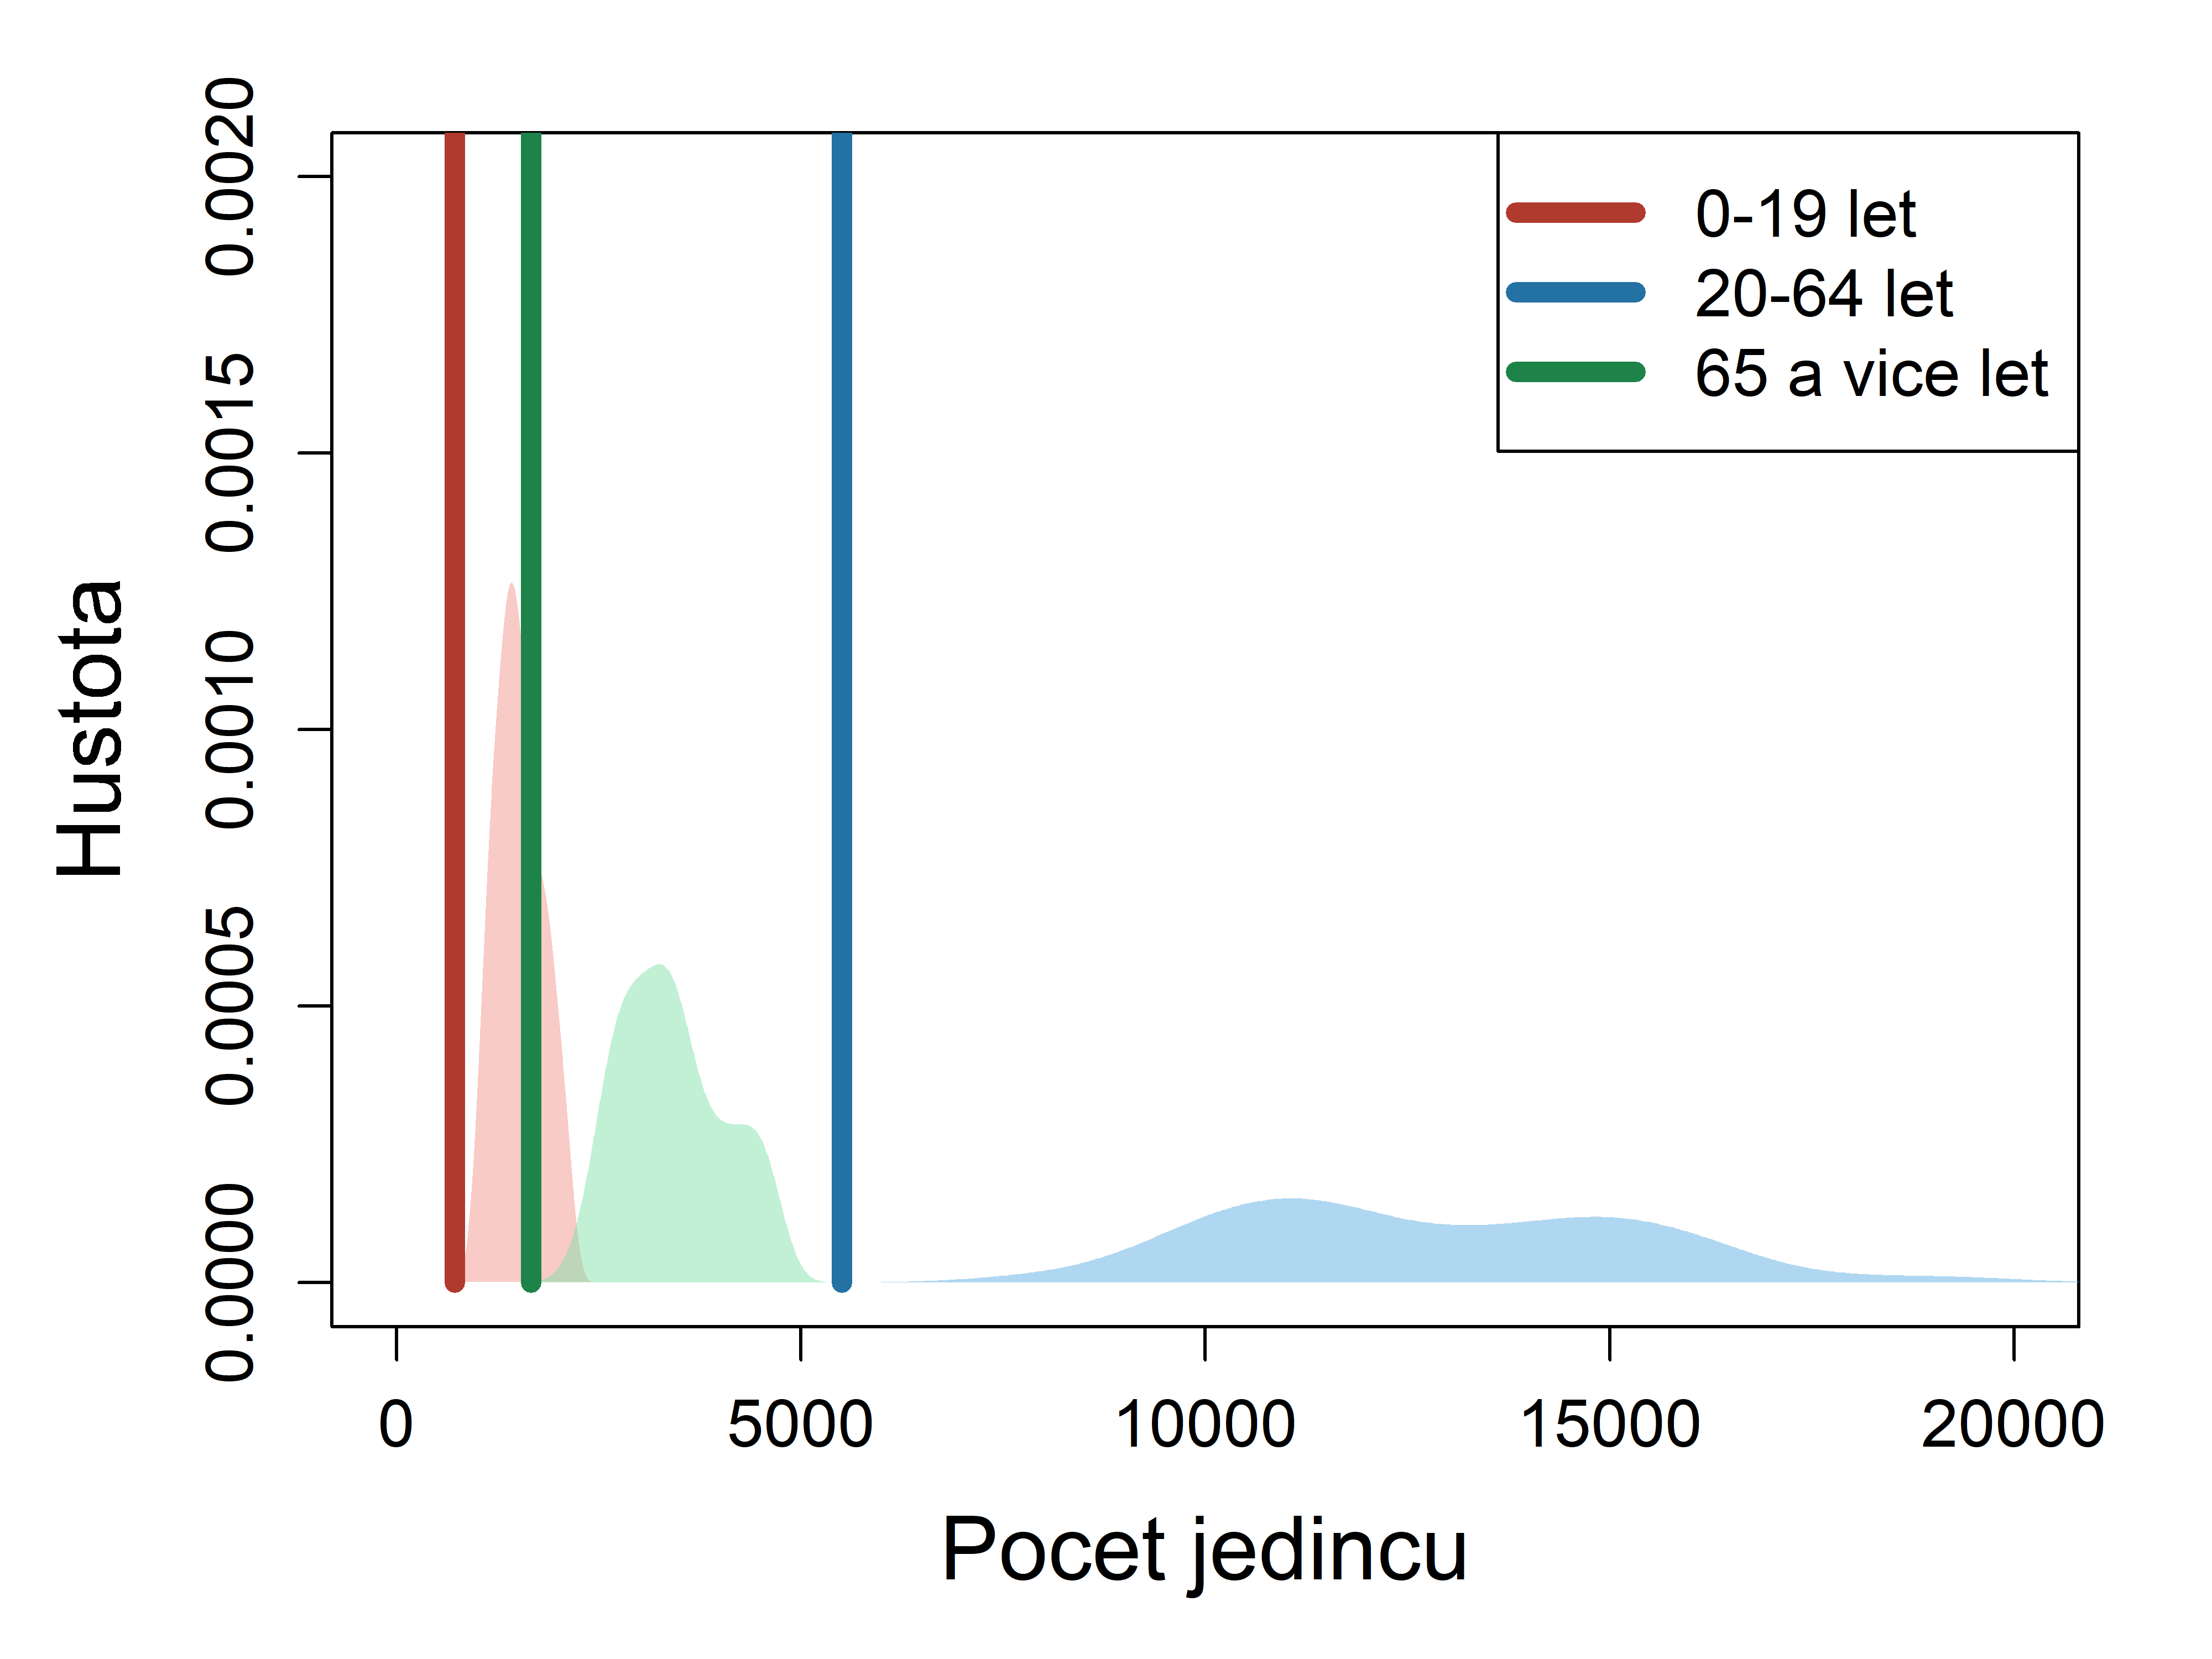
\includegraphics[width = \textwidth]{pic/sc_4later_PDF.png}
		\end{minipage}
	\end{center}
	\caption{Posun přijatých opatření v čase. Dynamika celkového počtu potvrzených případů za situace, kdy jsou všechna opatření přijata o čtyři dny dříve (A-B) nebo o čtyři dny později (C-D). Modré křivky v levých panelech reprezentují skutečná pozorování, kdežto oranžové křivky jsou výsledky 100 „nejlepších“ modelových simulací. Pravý panel ukazuje hustotní rozložení věkově specifických počtů potvrzených případů ve třech uvažovaných věkových třídách k 7.\ květnu 2020; vertikální čáry jsou skutečně pozorované počty, zatímco světlé plochy jsou distribuce vytvořené na základě modelových simulací odpovídajících levým panelům.}
	\label{scenariosR1R2}
\end{figure}

Druhý scénář odráží dlouho nekončící úvahy o tom, že plošná opatření nejsou opodstatněná, že jedinou smysluplnou strategií je co nejvíce omezit kontakty směrem k nejstarším věkovým skupinám, ve kterých umírá největší procento nakažených, a ostatní jedince nechat víceméně normálně žít. Tato strategie, na první pohled rozumná, je nesmyslná ze dvou důvodů. Z psychologického hlediska lidé v seniorním věku trpěli už při stávající intenzitě opatření, odpovídající zhruba 35 \% prepandemického stavu (tedy redukci o 65 \%), a není proto příliš představitelné tyto kontakty dále (plošně) omezovat. Co je však zřejmě důležitější, tato strategie nedává smysl ani z epidemiologického hlediska, jak ukazuje obr.\,\ref{shelterning_seniors}. Změna charakteru opatření nemá zpočátku na počty nemocných seniorů příliš znatelný efekt, avšak zhruba od poloviny dubna dochází v této věkové kategorii k masivnímu nárůstu nemocných. Důvodem je už od počátku značný nárůst nemocných v ostatních věkových skupinách a díky těmto velkým číslům následné proniknutí infekčních jedinců i mezi silně izolovanou kohortu seniorů (obr.\,\ref{shelterning_seniors}).

\begin{figure}
	\begin{center}
		\begin{minipage}[t]{0.45\textwidth}
			A) \\
			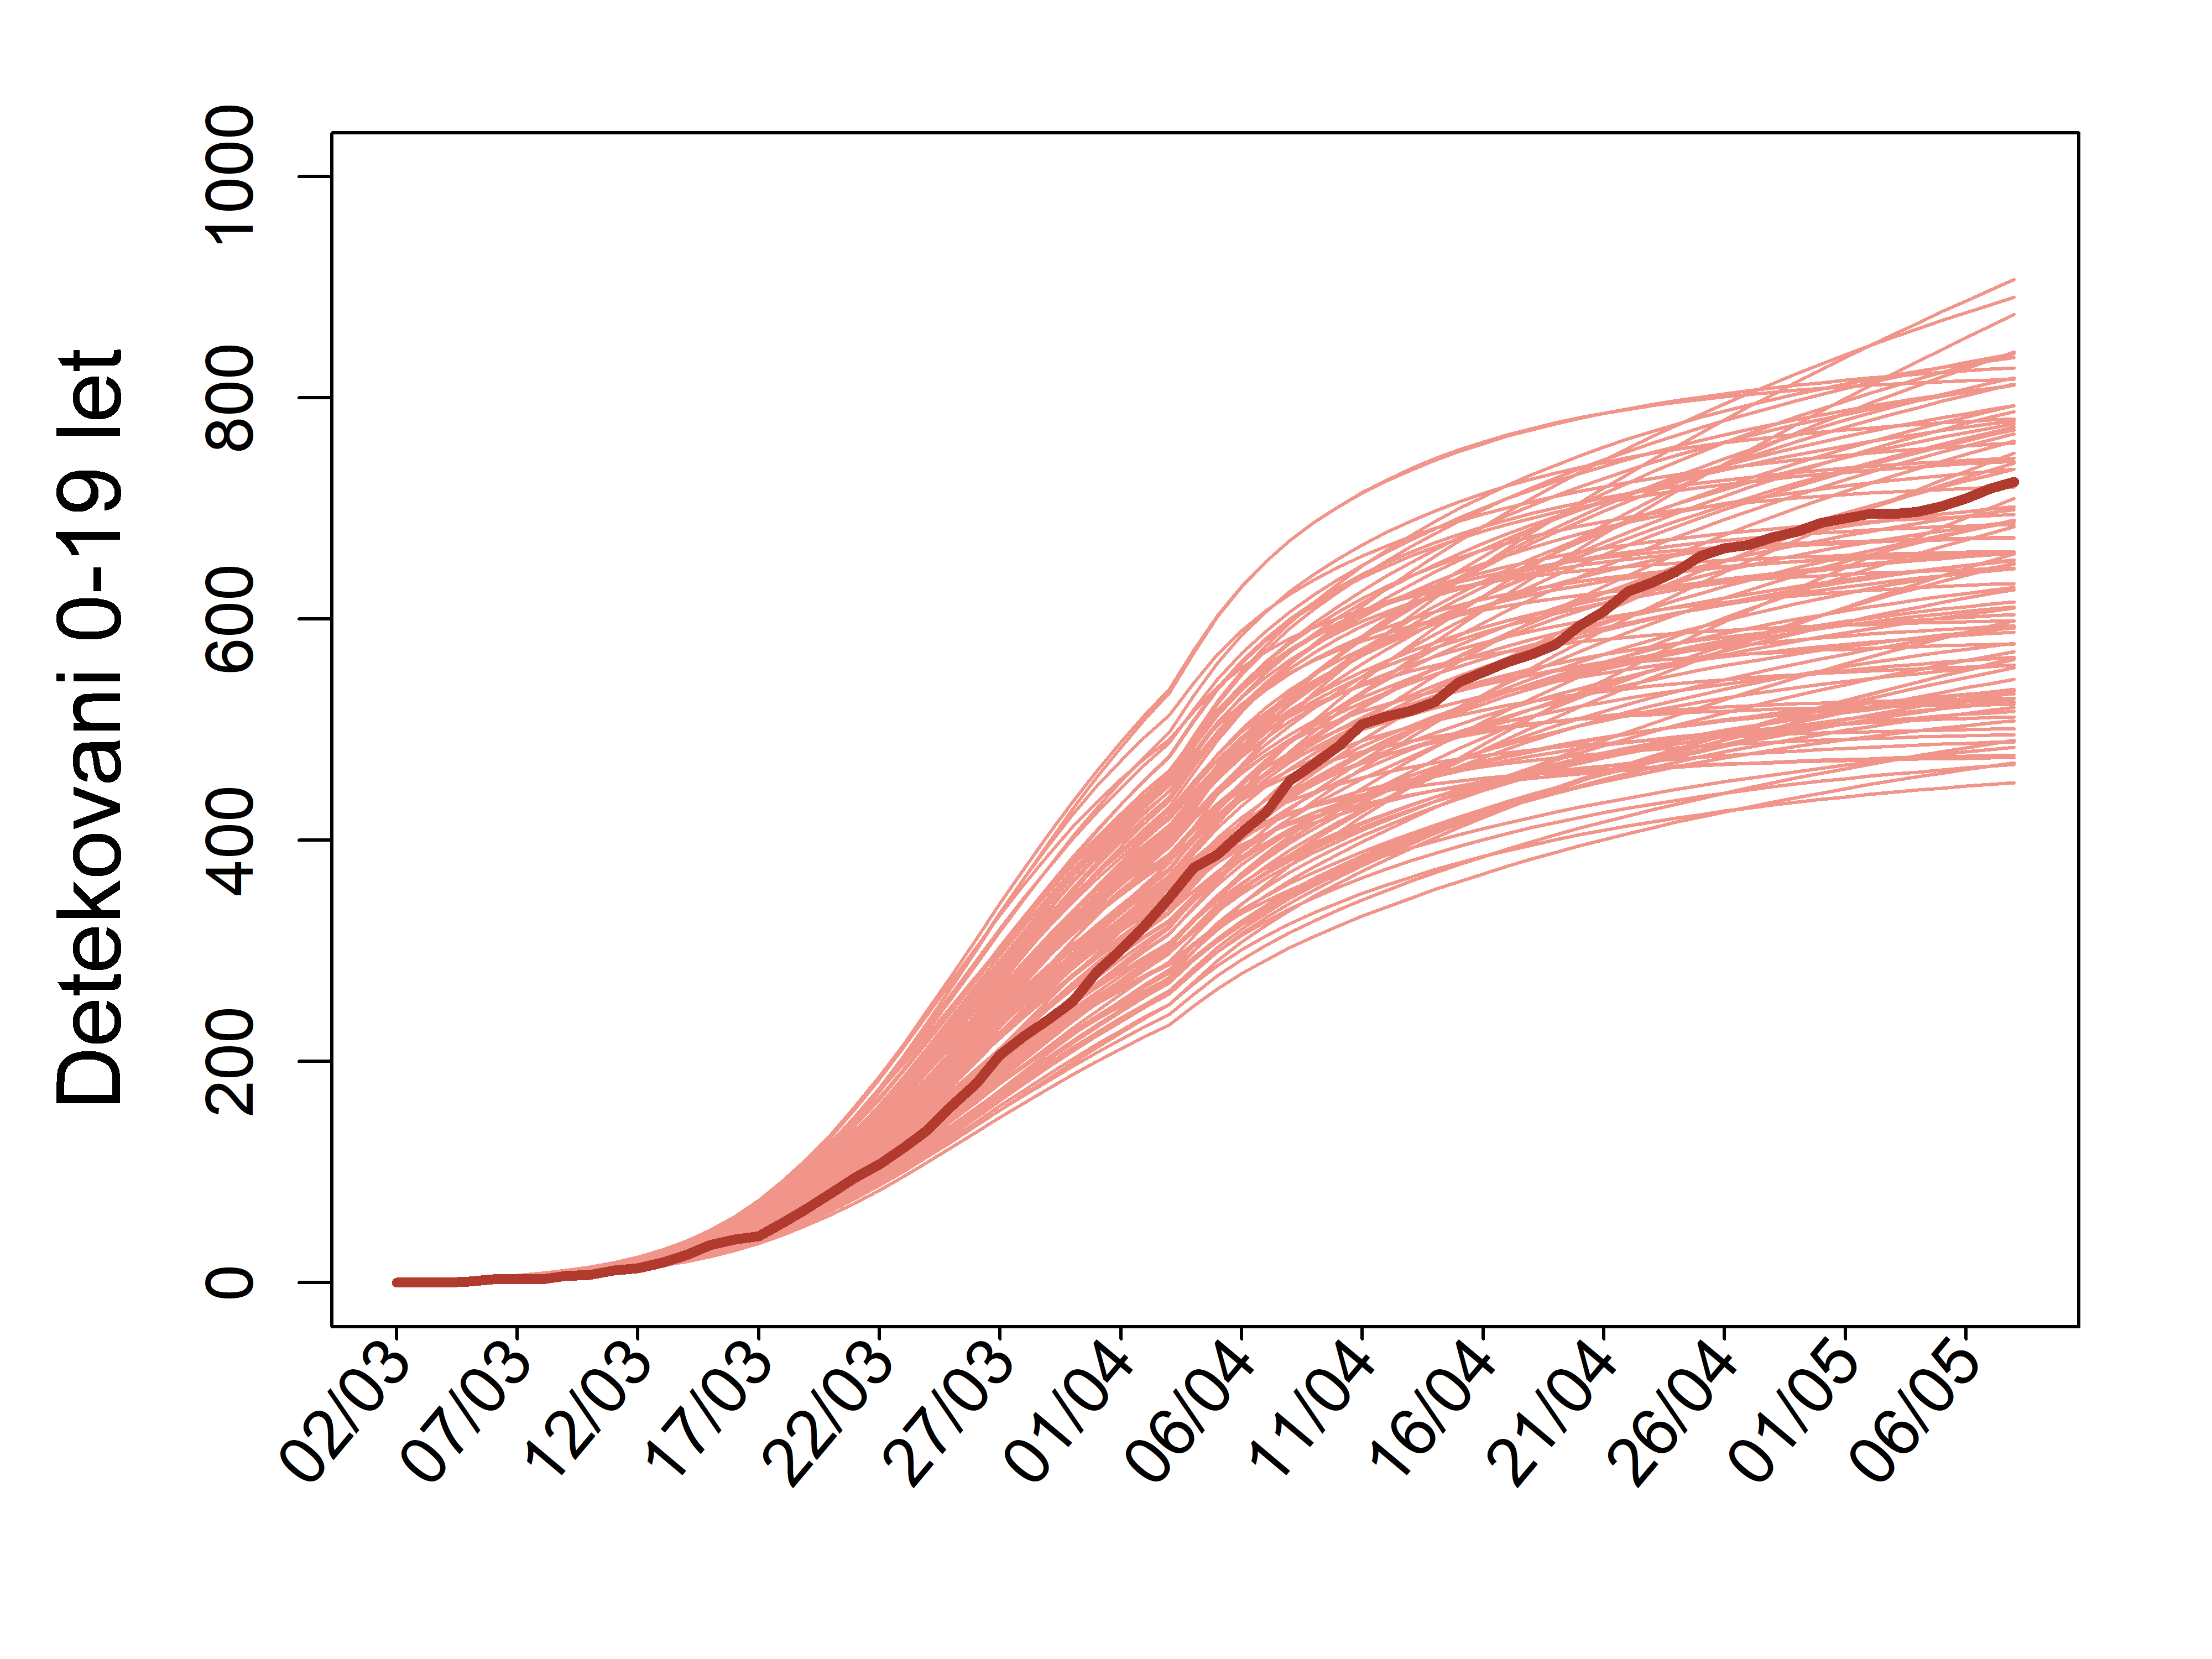
\includegraphics[width = \textwidth]{pic/sc_bas_1.png}
		\end{minipage}
		\begin{minipage}[t]{0.45\textwidth}
			B) \\
			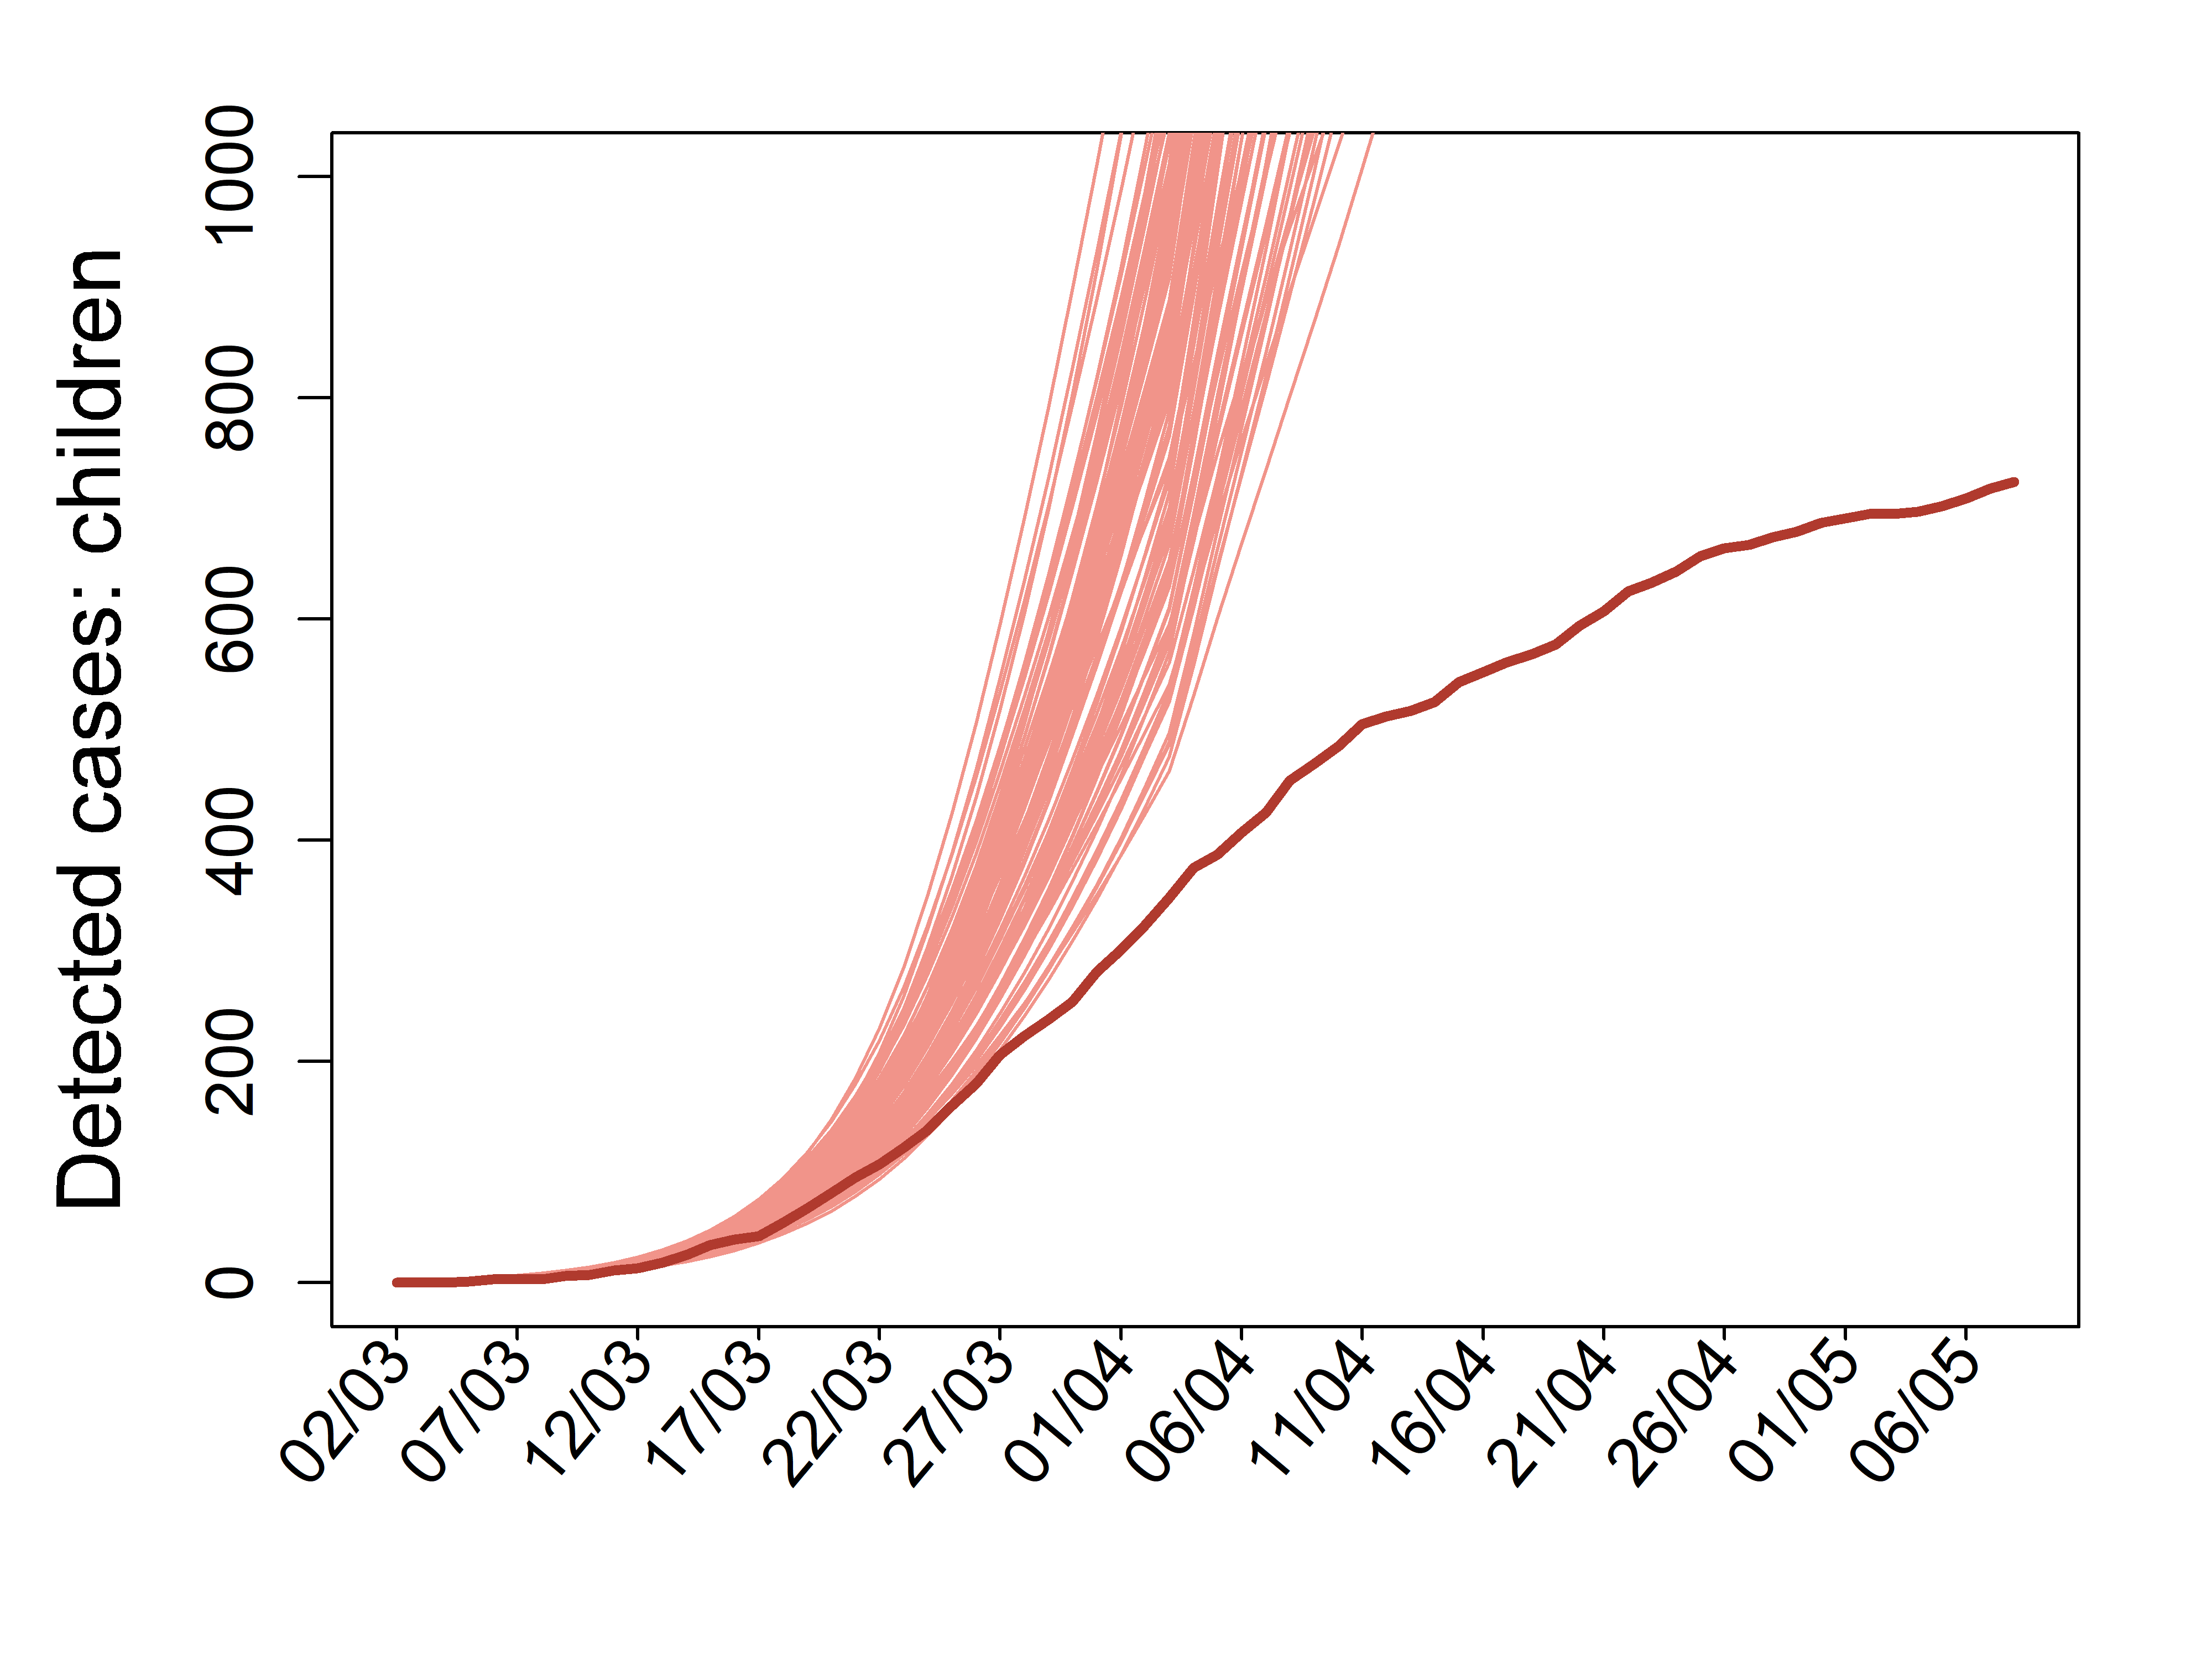
\includegraphics[width = \textwidth]{pic/sc_old90_30_1.png}
		\end{minipage}
		\begin{minipage}[m]{0.45\textwidth}
			C) \\
			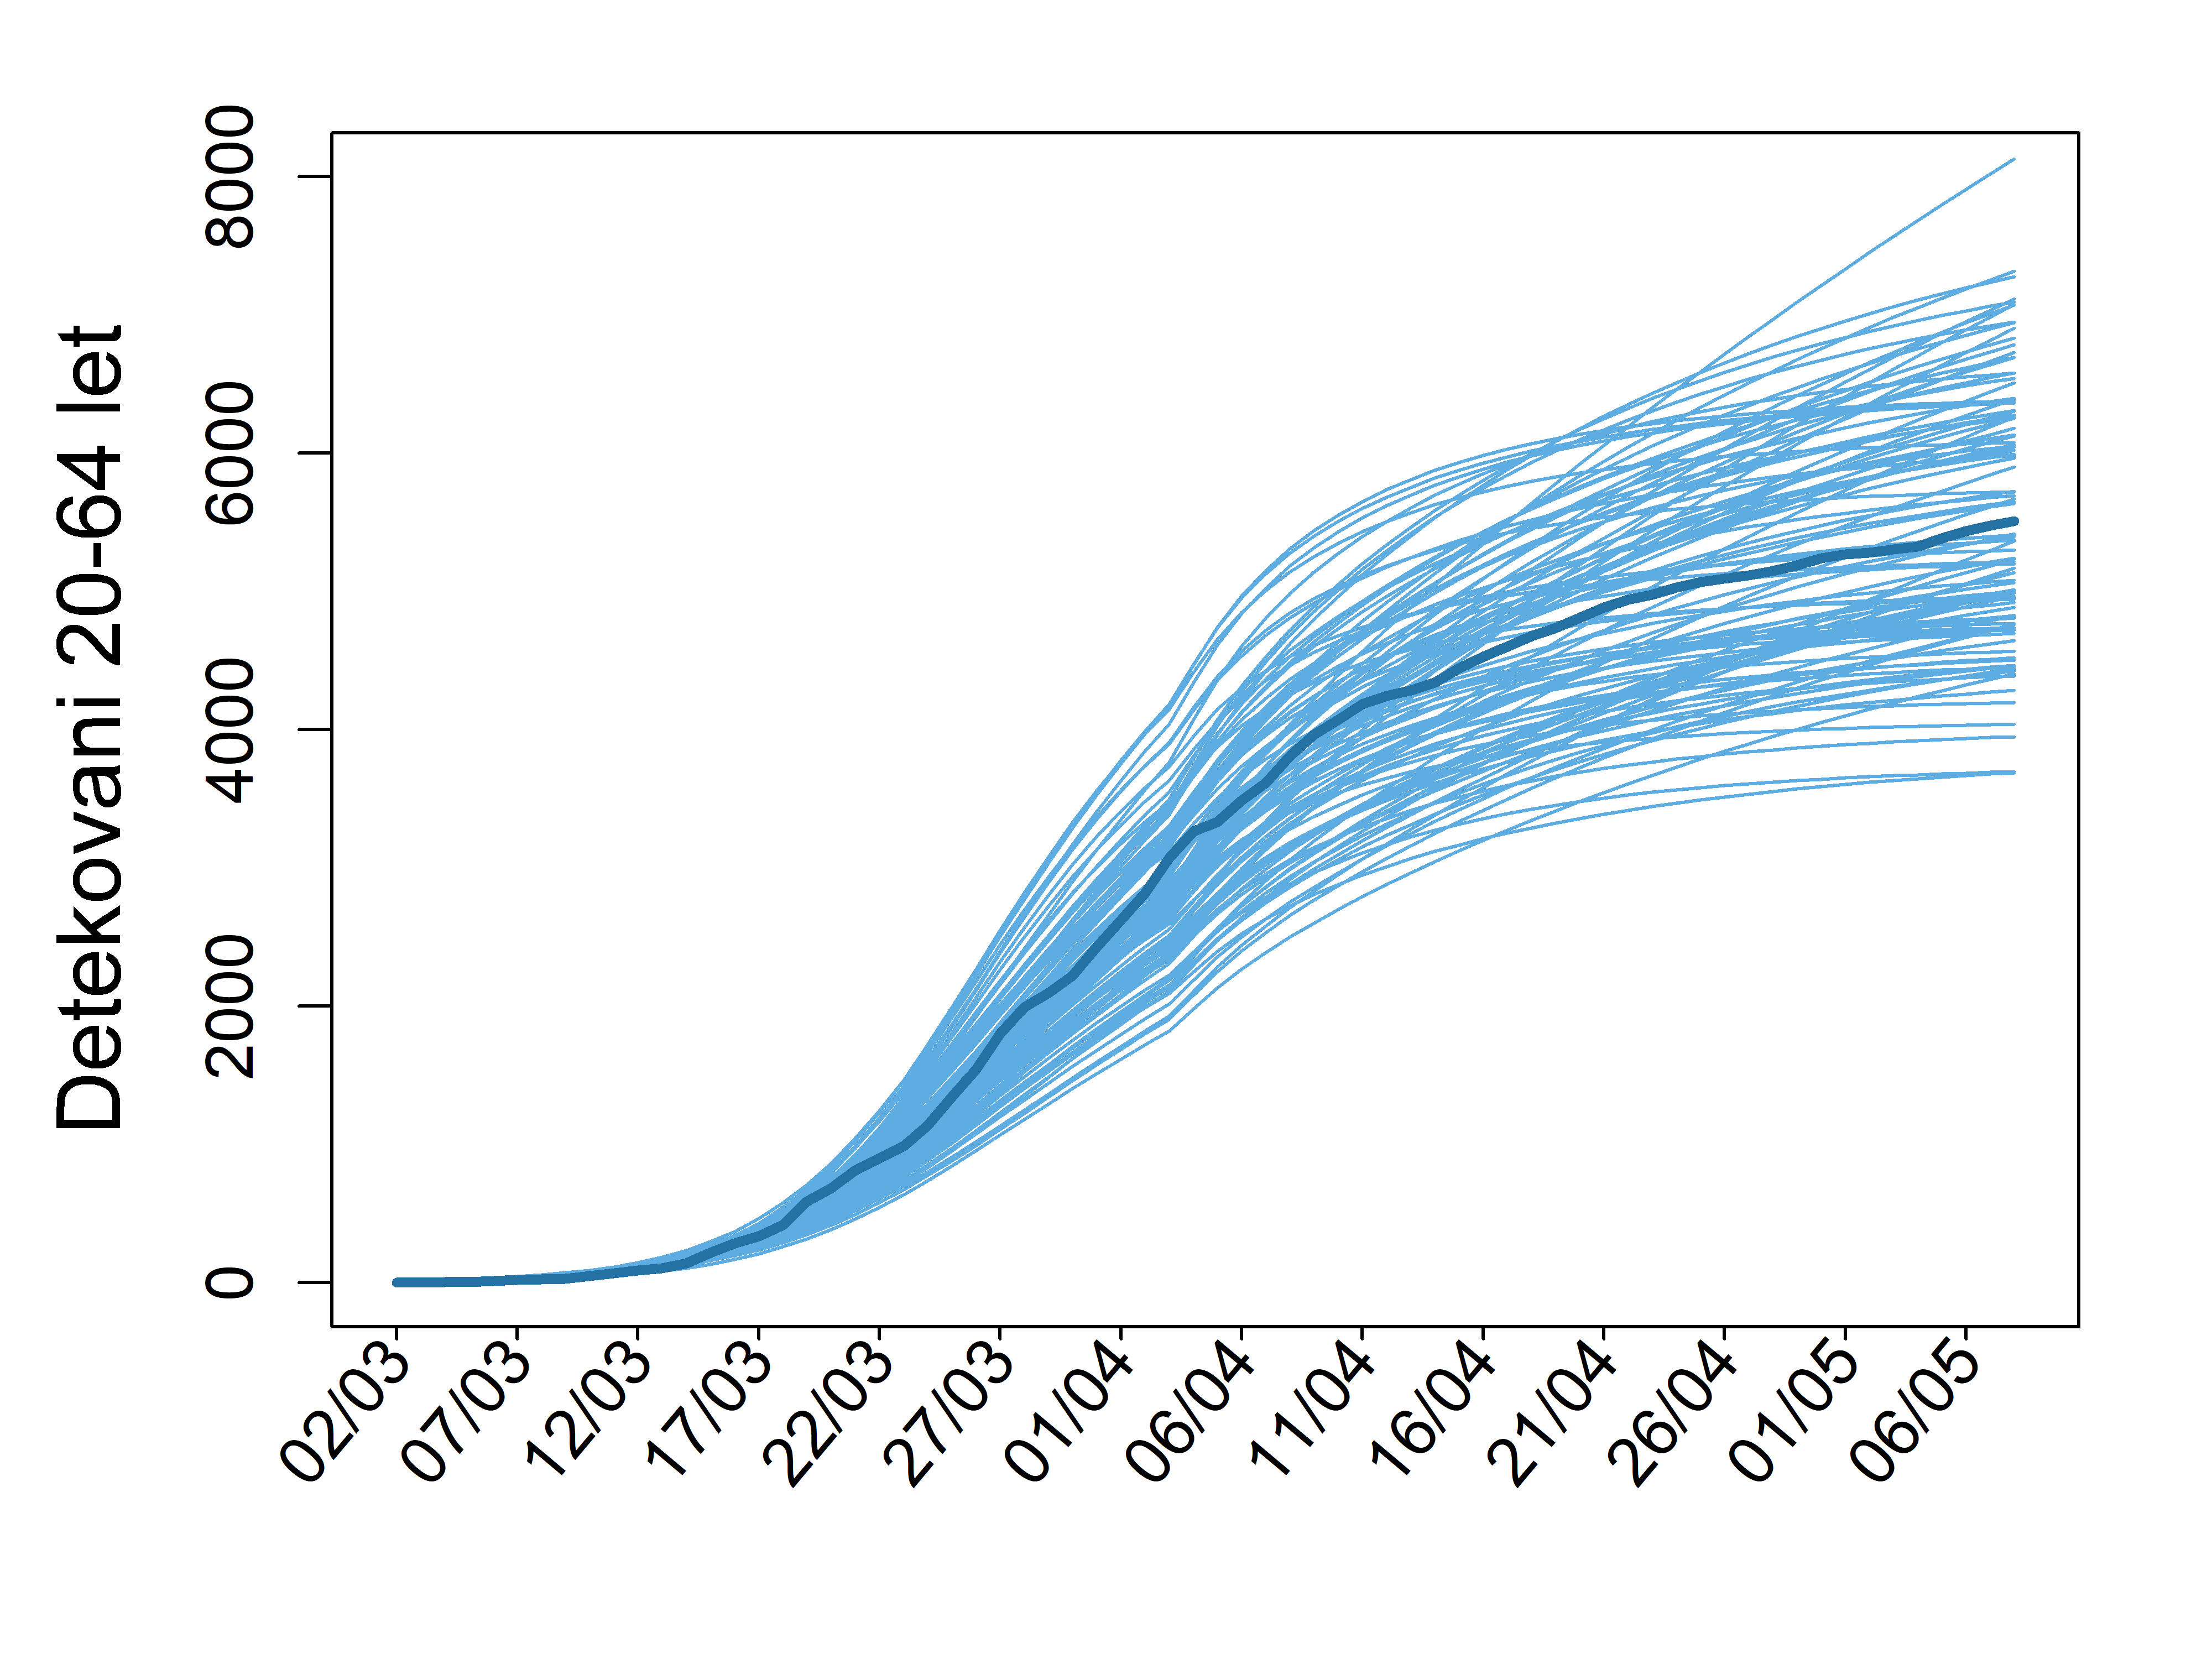
\includegraphics[width = \textwidth]{pic/sc_bas_2.png}
		\end{minipage}
		\begin{minipage}[m]{0.45\textwidth}
			D) \\
			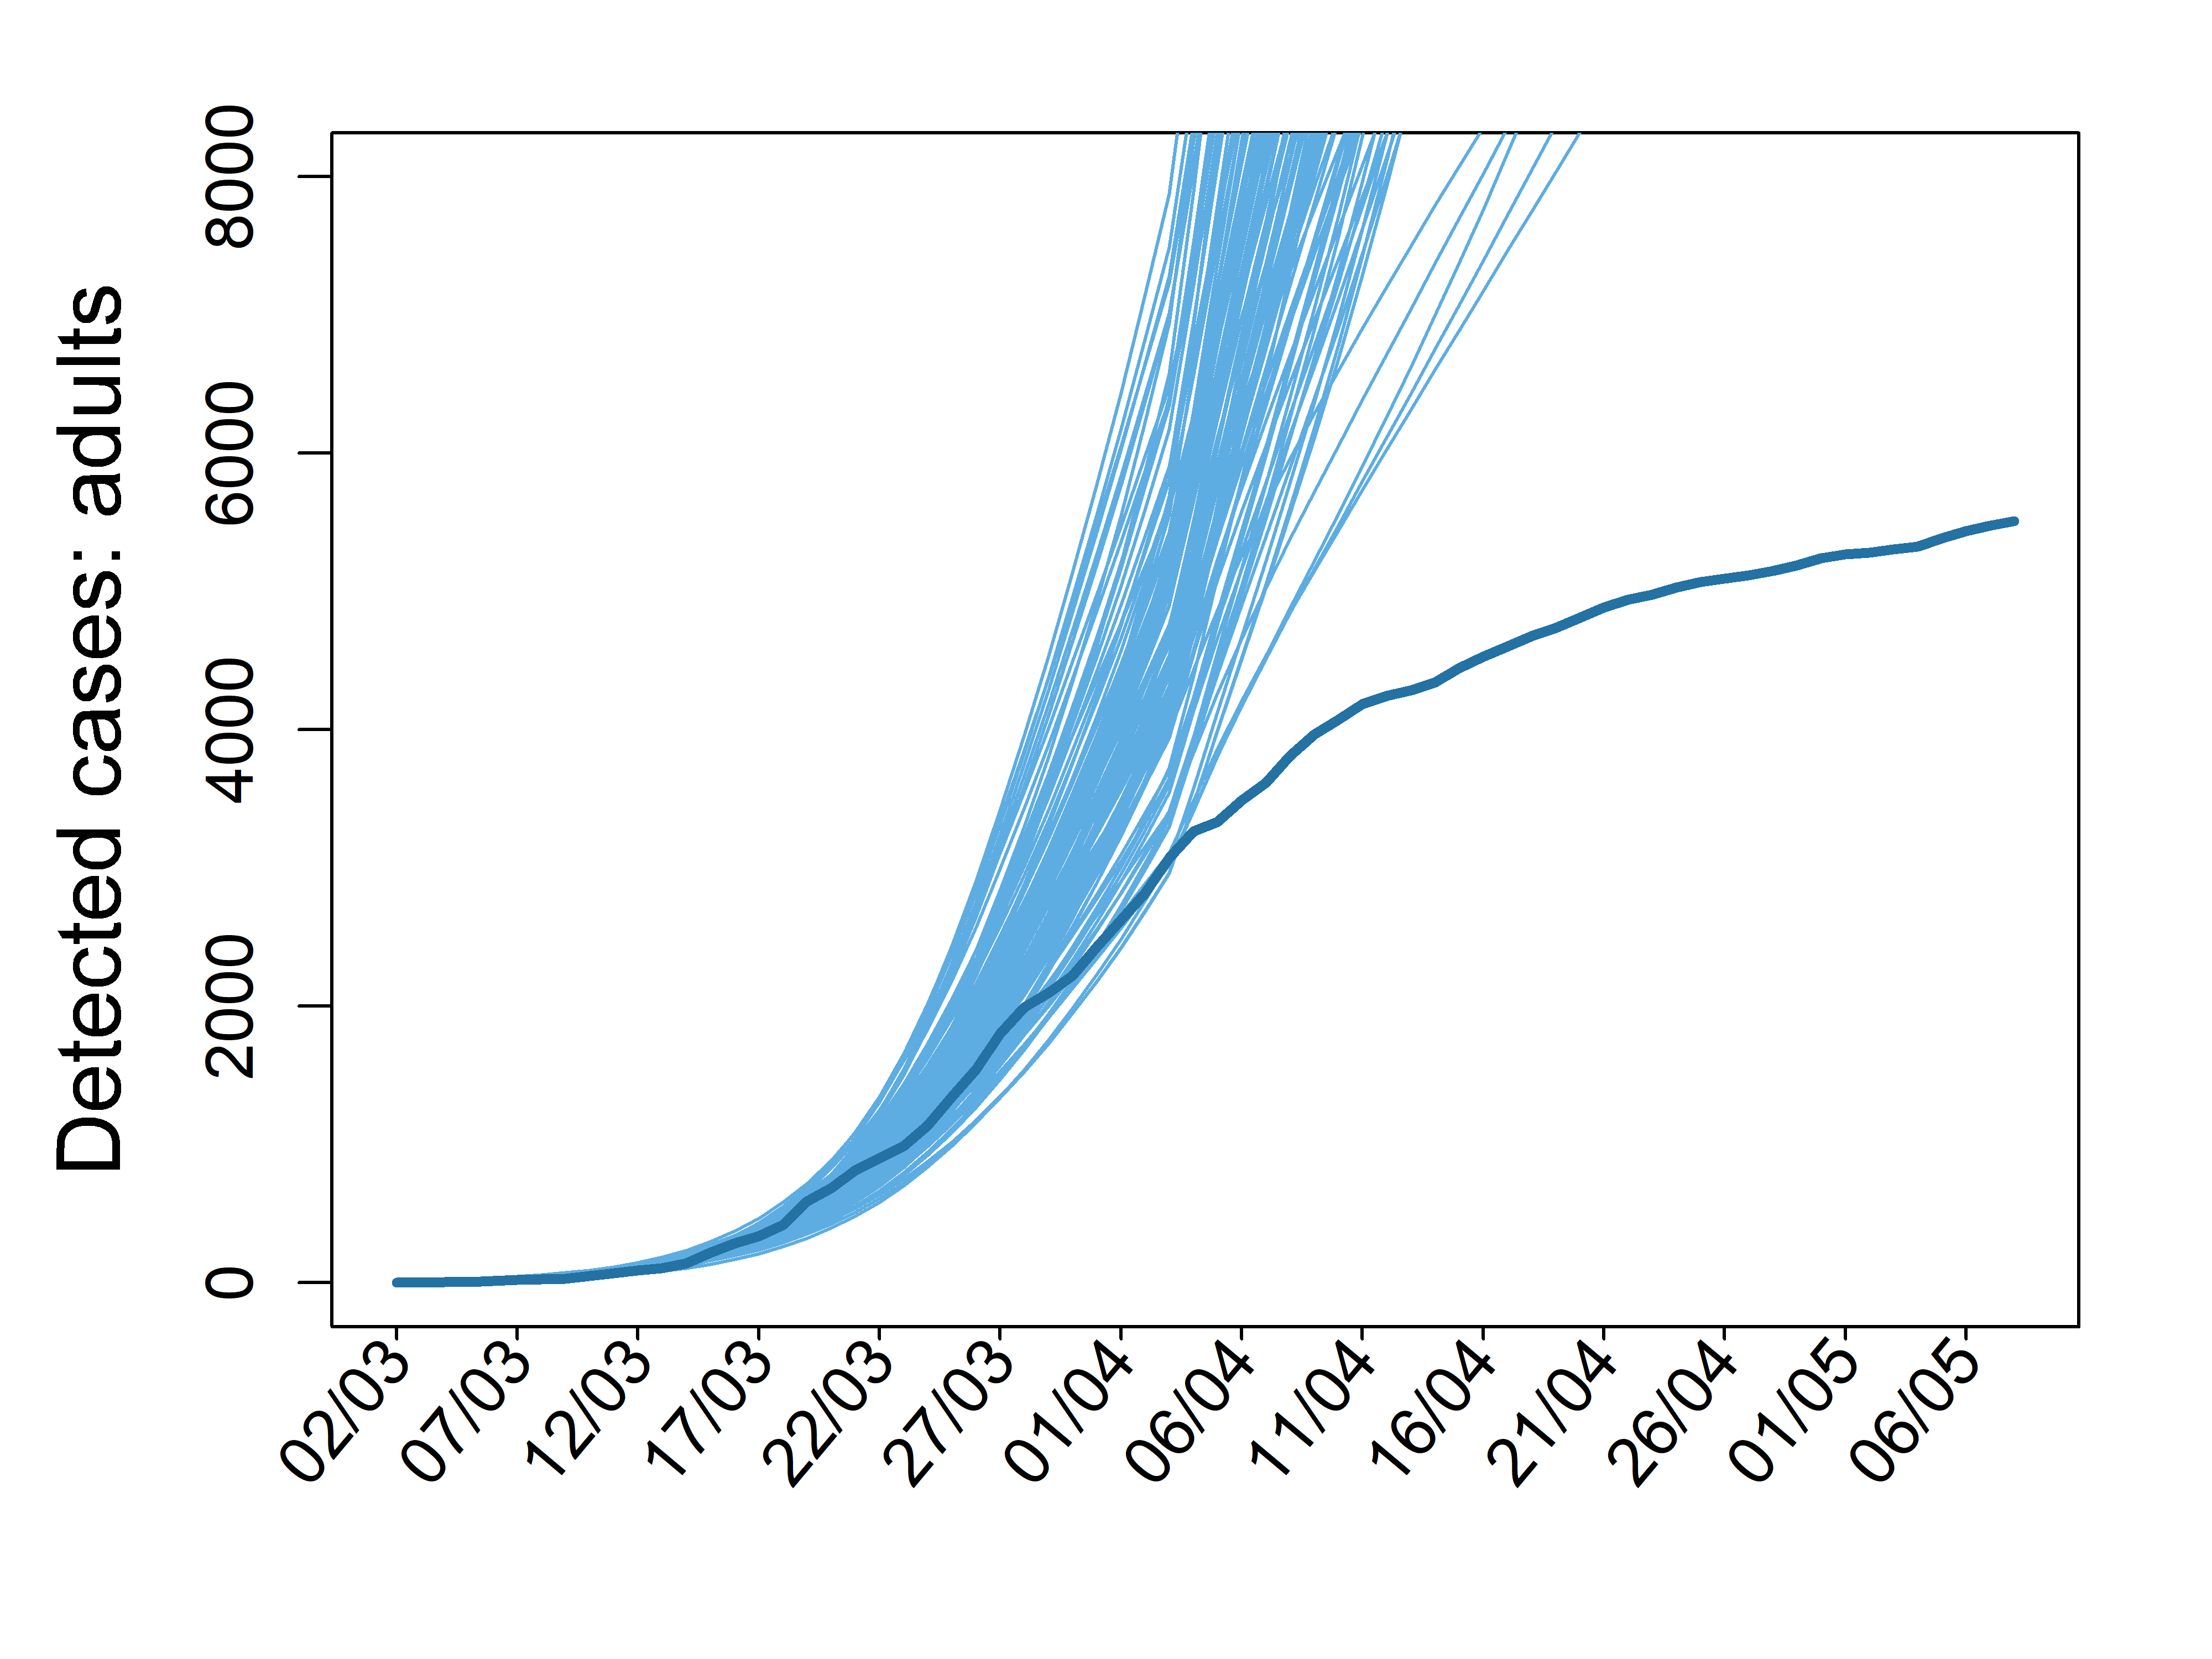
\includegraphics[width = \textwidth]{pic/sc_old90_30_2.png}
		\end{minipage} \\[1ex]
		\begin{minipage}[m]{0.45\textwidth}
			E) \\
			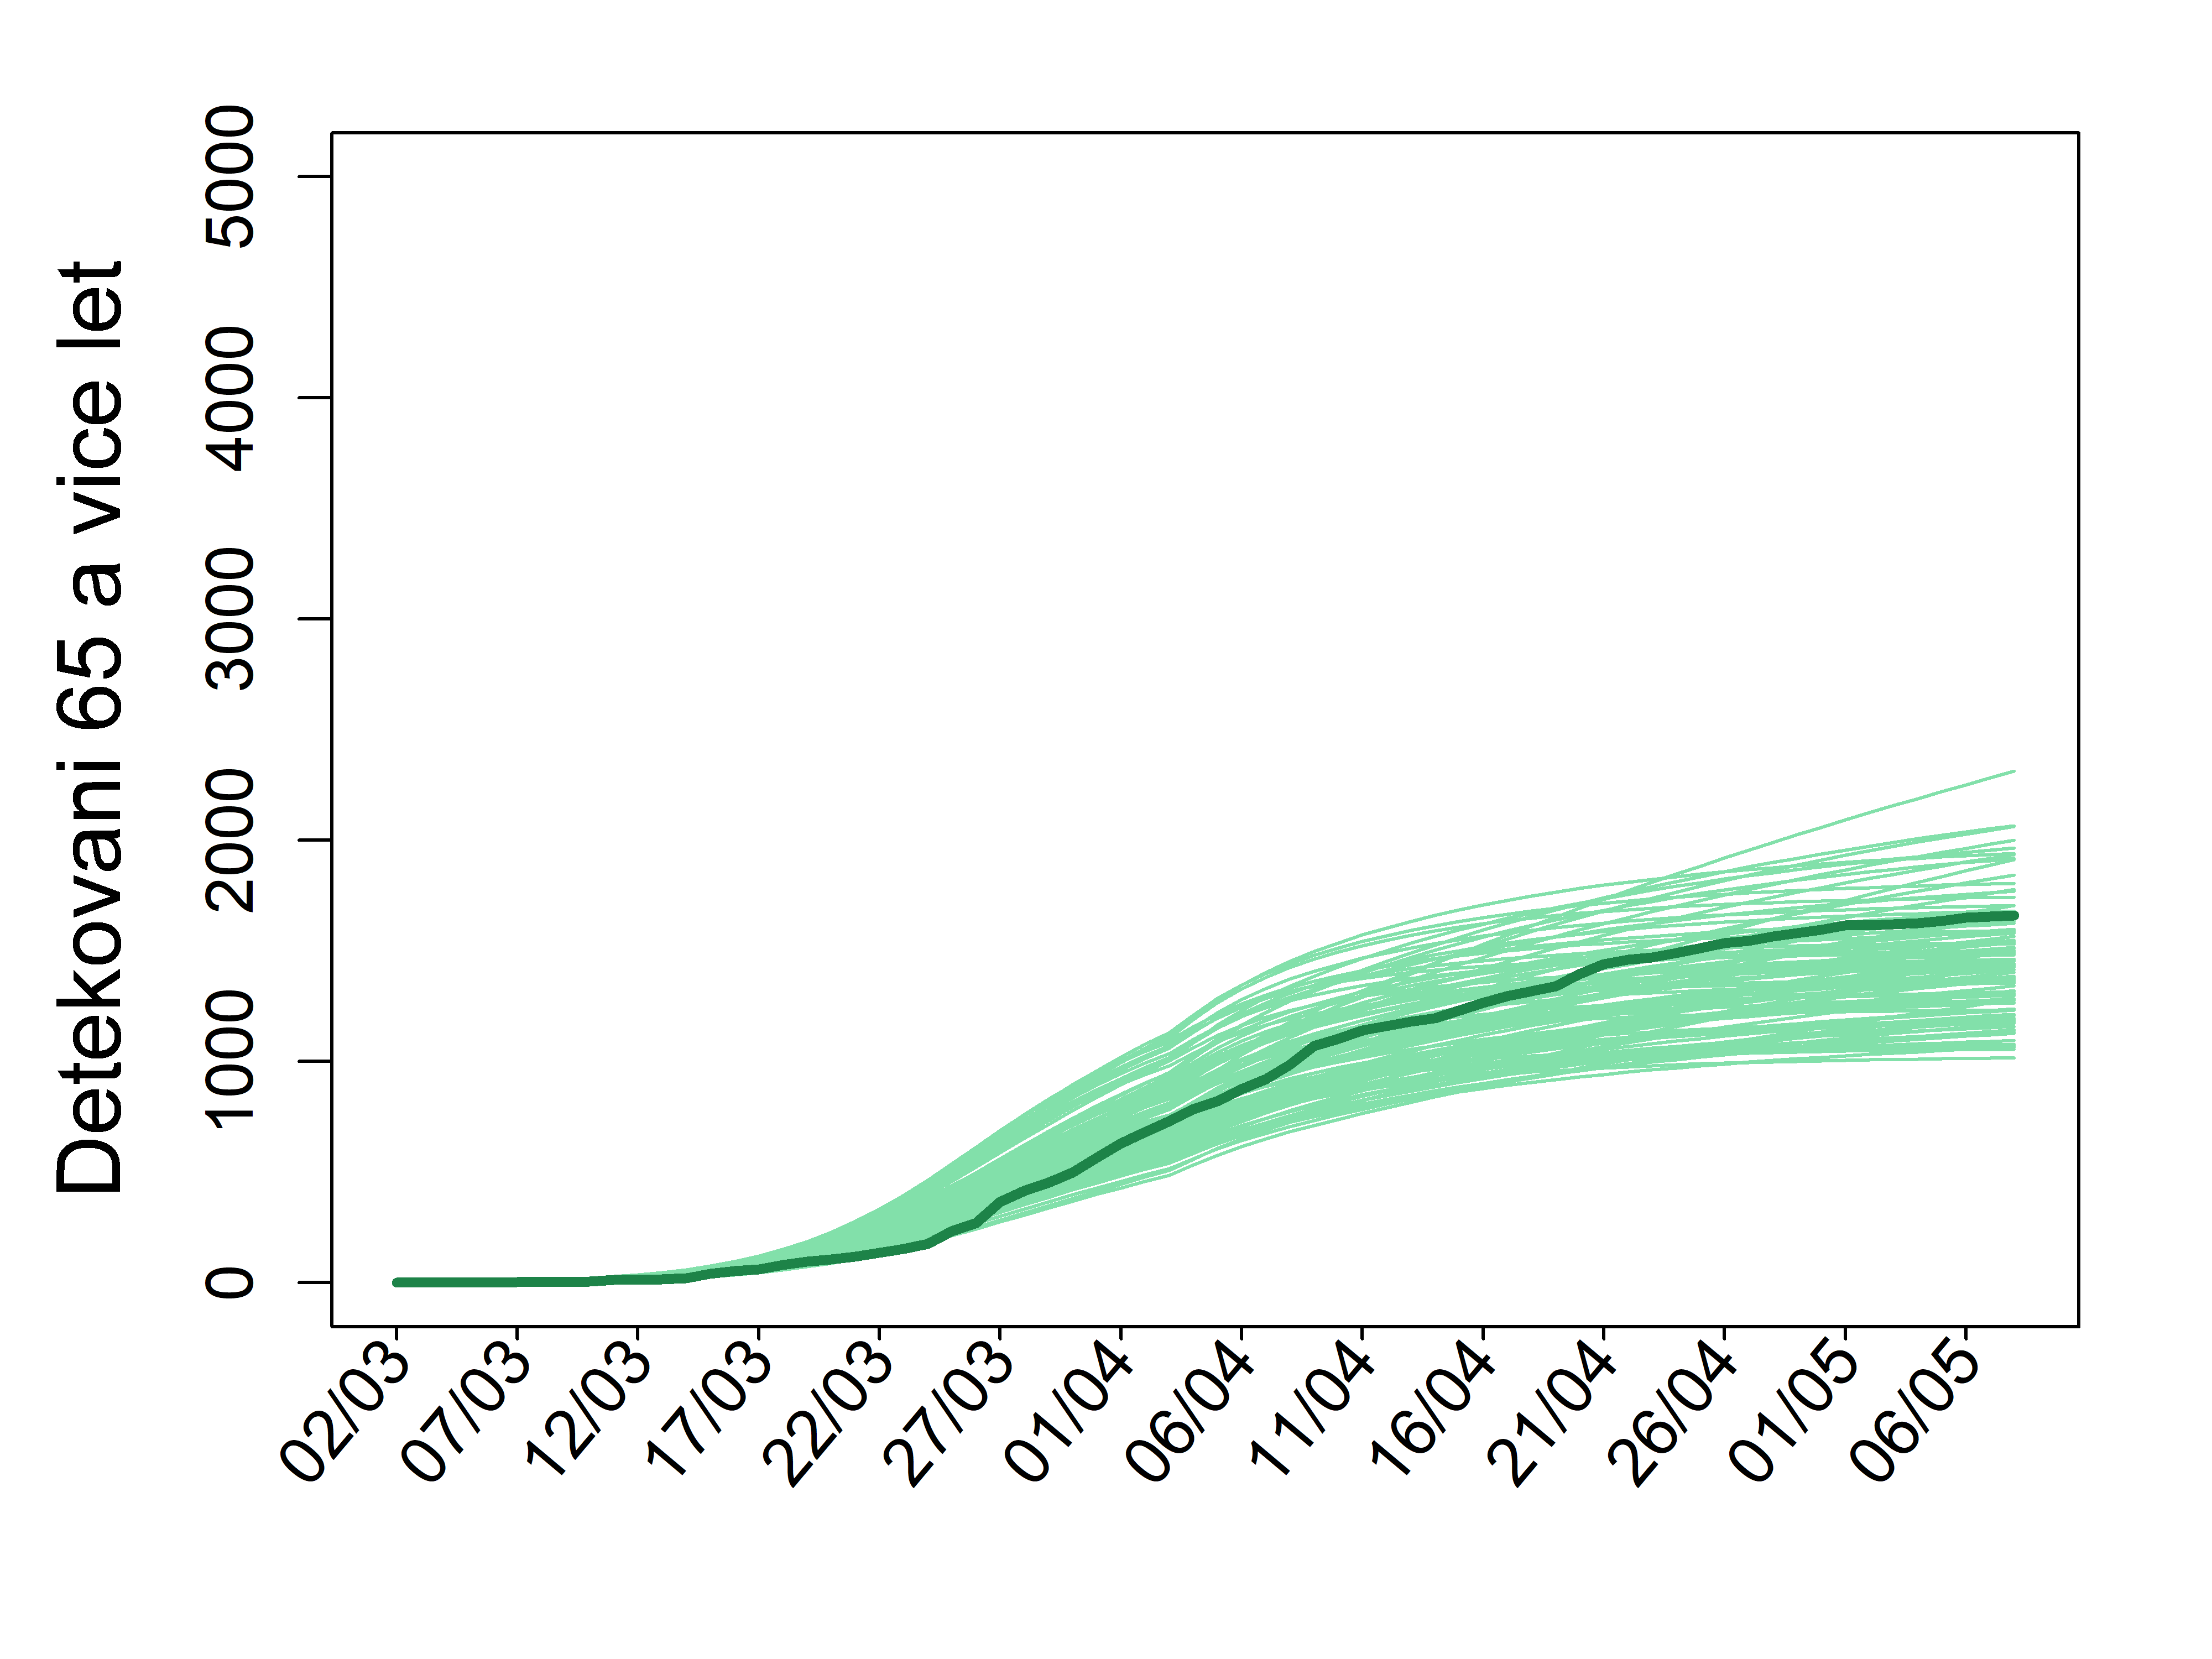
\includegraphics[width = \textwidth]{pic/sc_bas_3.png}
		\end{minipage}
		\begin{minipage}[m]{0.45\textwidth}
			F) \\
			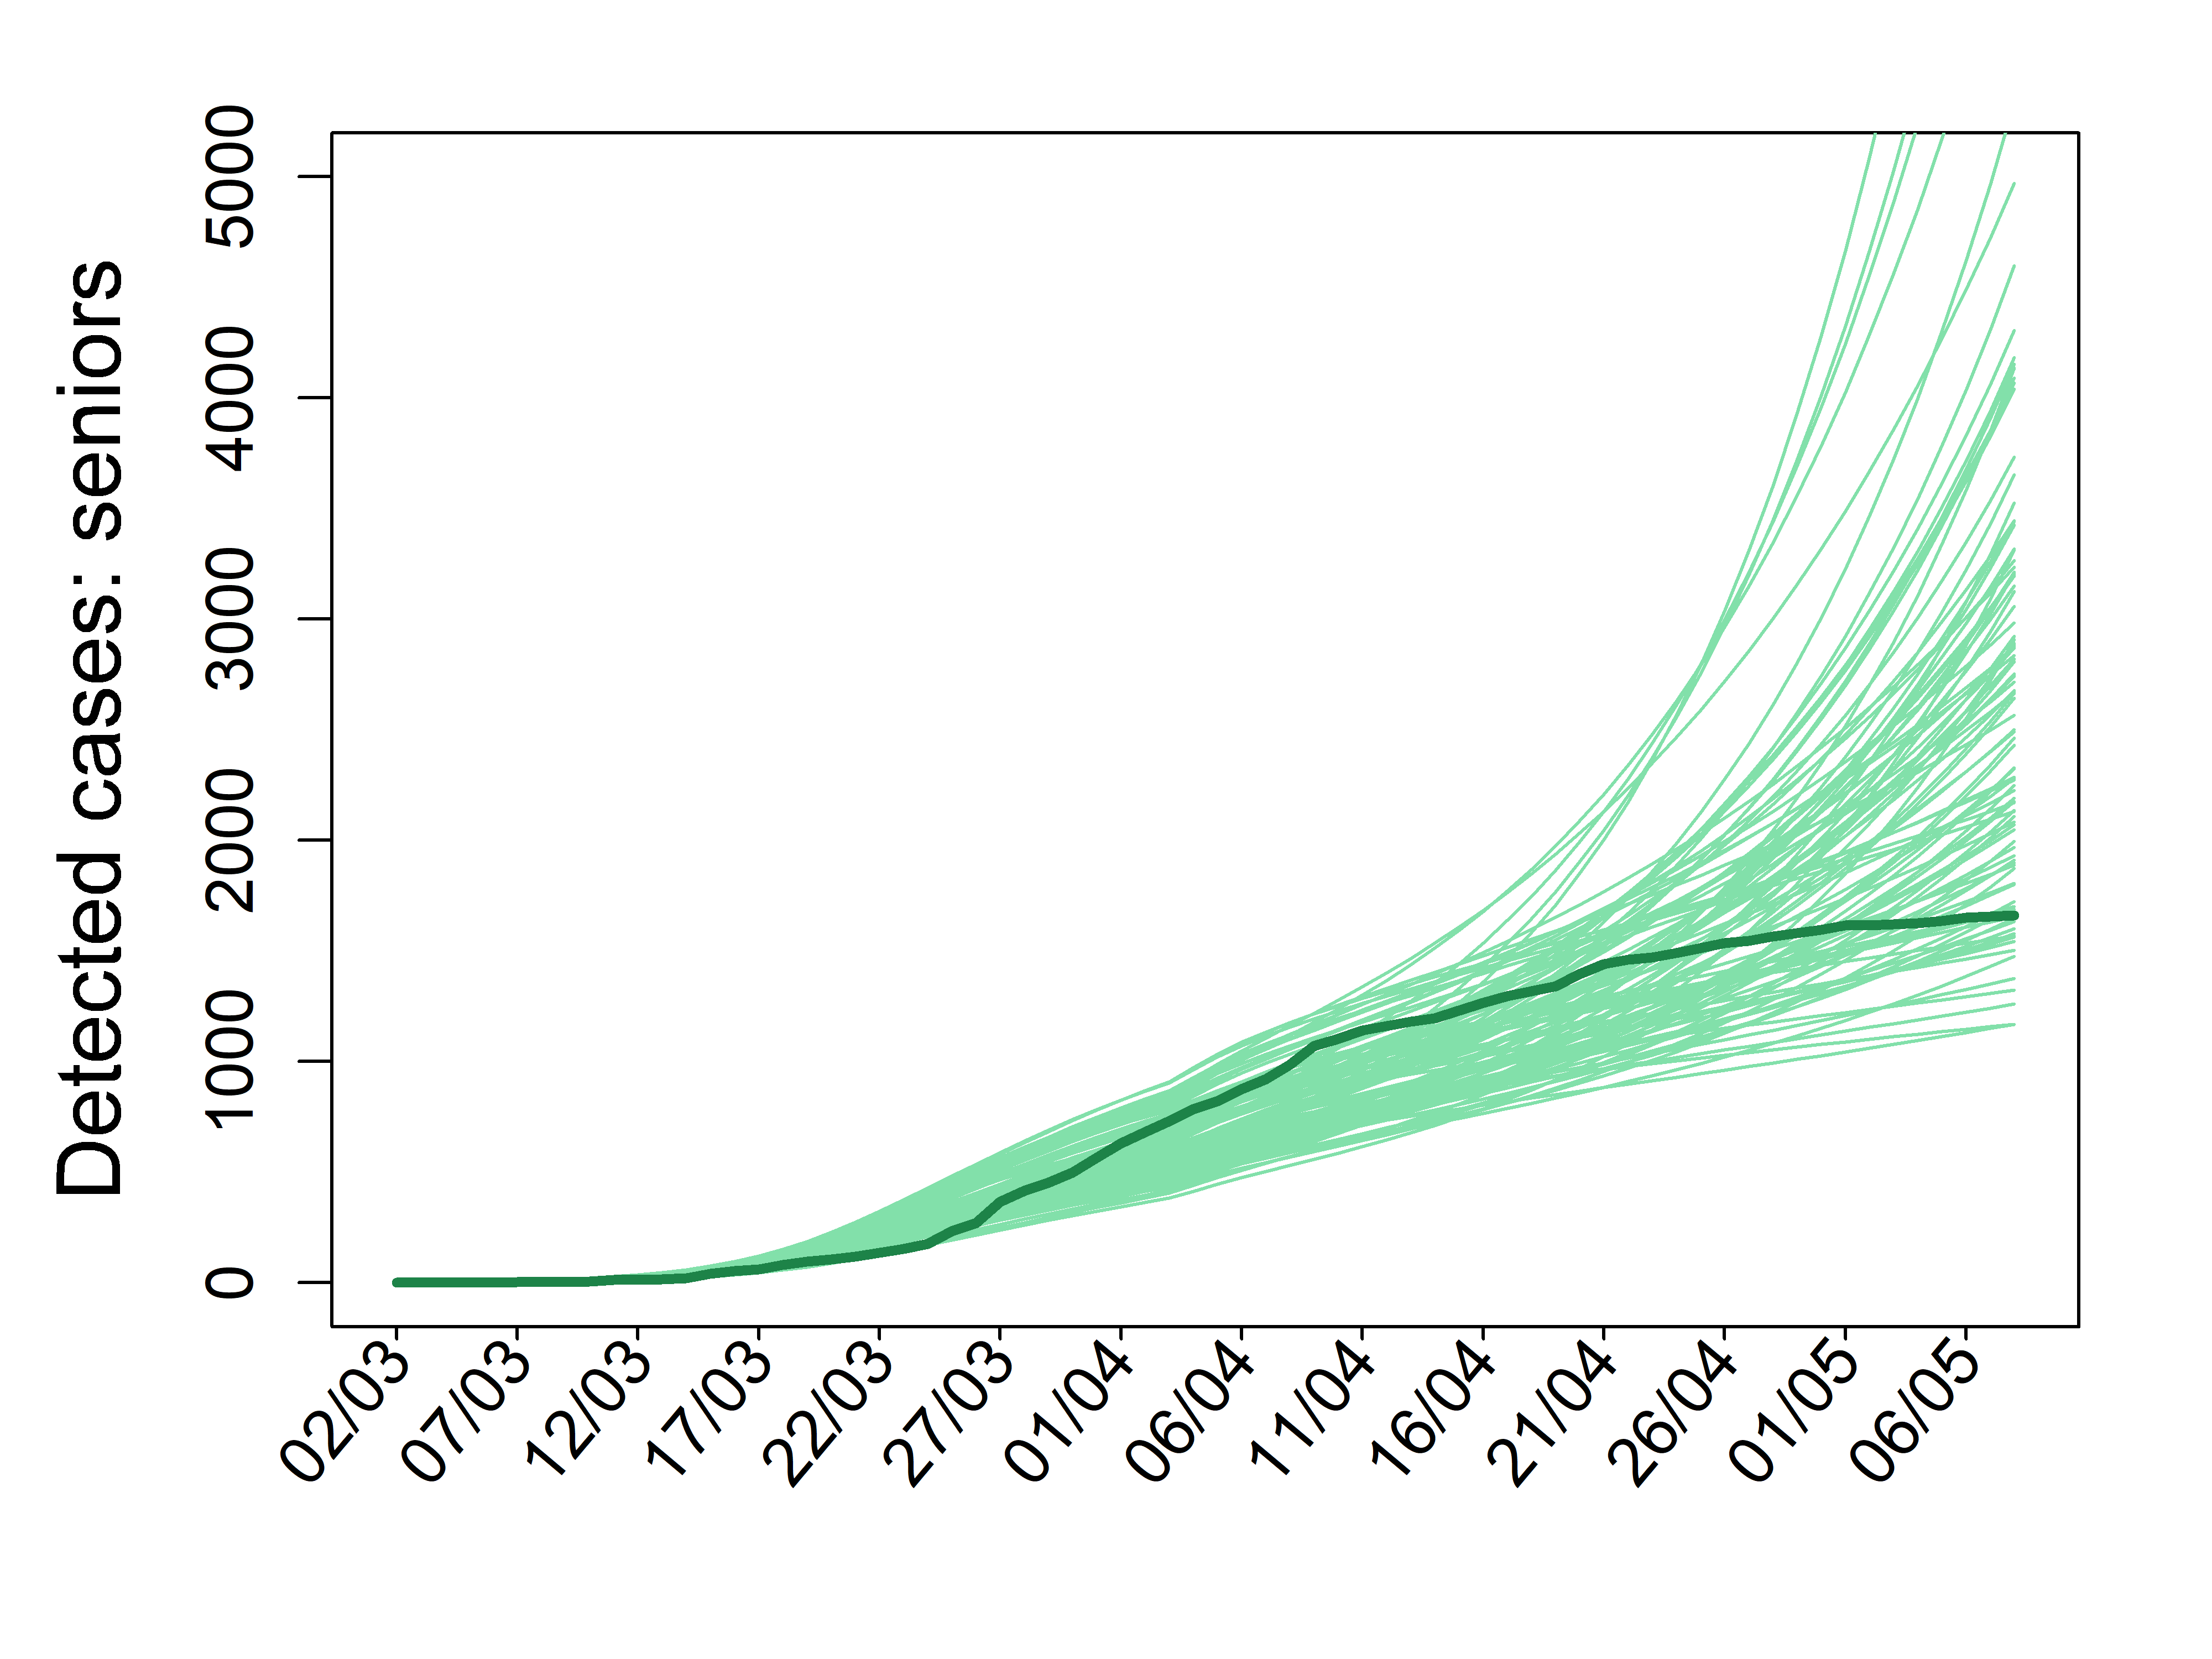
\includegraphics[width = \textwidth]{pic/sc_old90_30_3.png}
		\end{minipage}
	\end{center}
	\caption{Levý sloupec: kalibrace modelu na celkové počty potvrzených případů v jednotlivých uvažovaných věkových kategoriích. Pravý panel: výsledky simulací pro scénář, kdy jsou kontakty seniorů se zbytkem populace omezeny o 90 \%, zatímco kontakty v rámci neseniorní populace jsou omezeny pouze o 30 \%; senioři navíc dodržují zásady osobní ochrany z 90 \%, kdežto ostatní jen z 50 \%. Tmavé křivky v jednotlivých panelech reprezentují skutečná pozorování, kdežto tenké světlé křivky jsou výsledky 100 „nejlepších“ modelových simulací.}
	\label{shelterning_seniors}
\end{figure}

Jako poslední scénář uvažujme jiný sled opatření: zaměňme časové okamžiky zavedení osobních ochranných opatření (poslední řádek tab.\,\ref{table:interventions}) a zavření škol a doporučení práce z domova (první řádek tab.\,\ref{table:interventions}). Jak ukazuje obr.\,\ref{switch}, efekt pořadí je výrazný: včasné zavedení osobní ochrany výrazně omezuje dopad epidemie, i když školy zavřeme mnohem později. Výsledky také naznačují, že i pouze částečné zavření škol by v takové situaci stále mohlo vést k nižším počtům případů než skutečně pozorovaných. Obr.\,\ref{switch} také ukazuje, jak by mohl vypadat průběh epidemie v případě, že by na počátku epidemie bylo efektivnější testování z hlediska časové prodlevy mezi vznikem symptomů a reportováním v případě pozitivity. Zatímco v březnu 2020 bylo toto prodlení průměrně 6,1 dne, v dubnu a květnu 2020 toto číslo kleslo na 2,9 dne. Obr.\,\ref{switch} předpokládá, že hodnota 2,9 dne je platná také pro březen 2020.

\begin{figure}
	\begin{center}
		\begin{minipage}[m]{0.45\textwidth}
			A) \\
			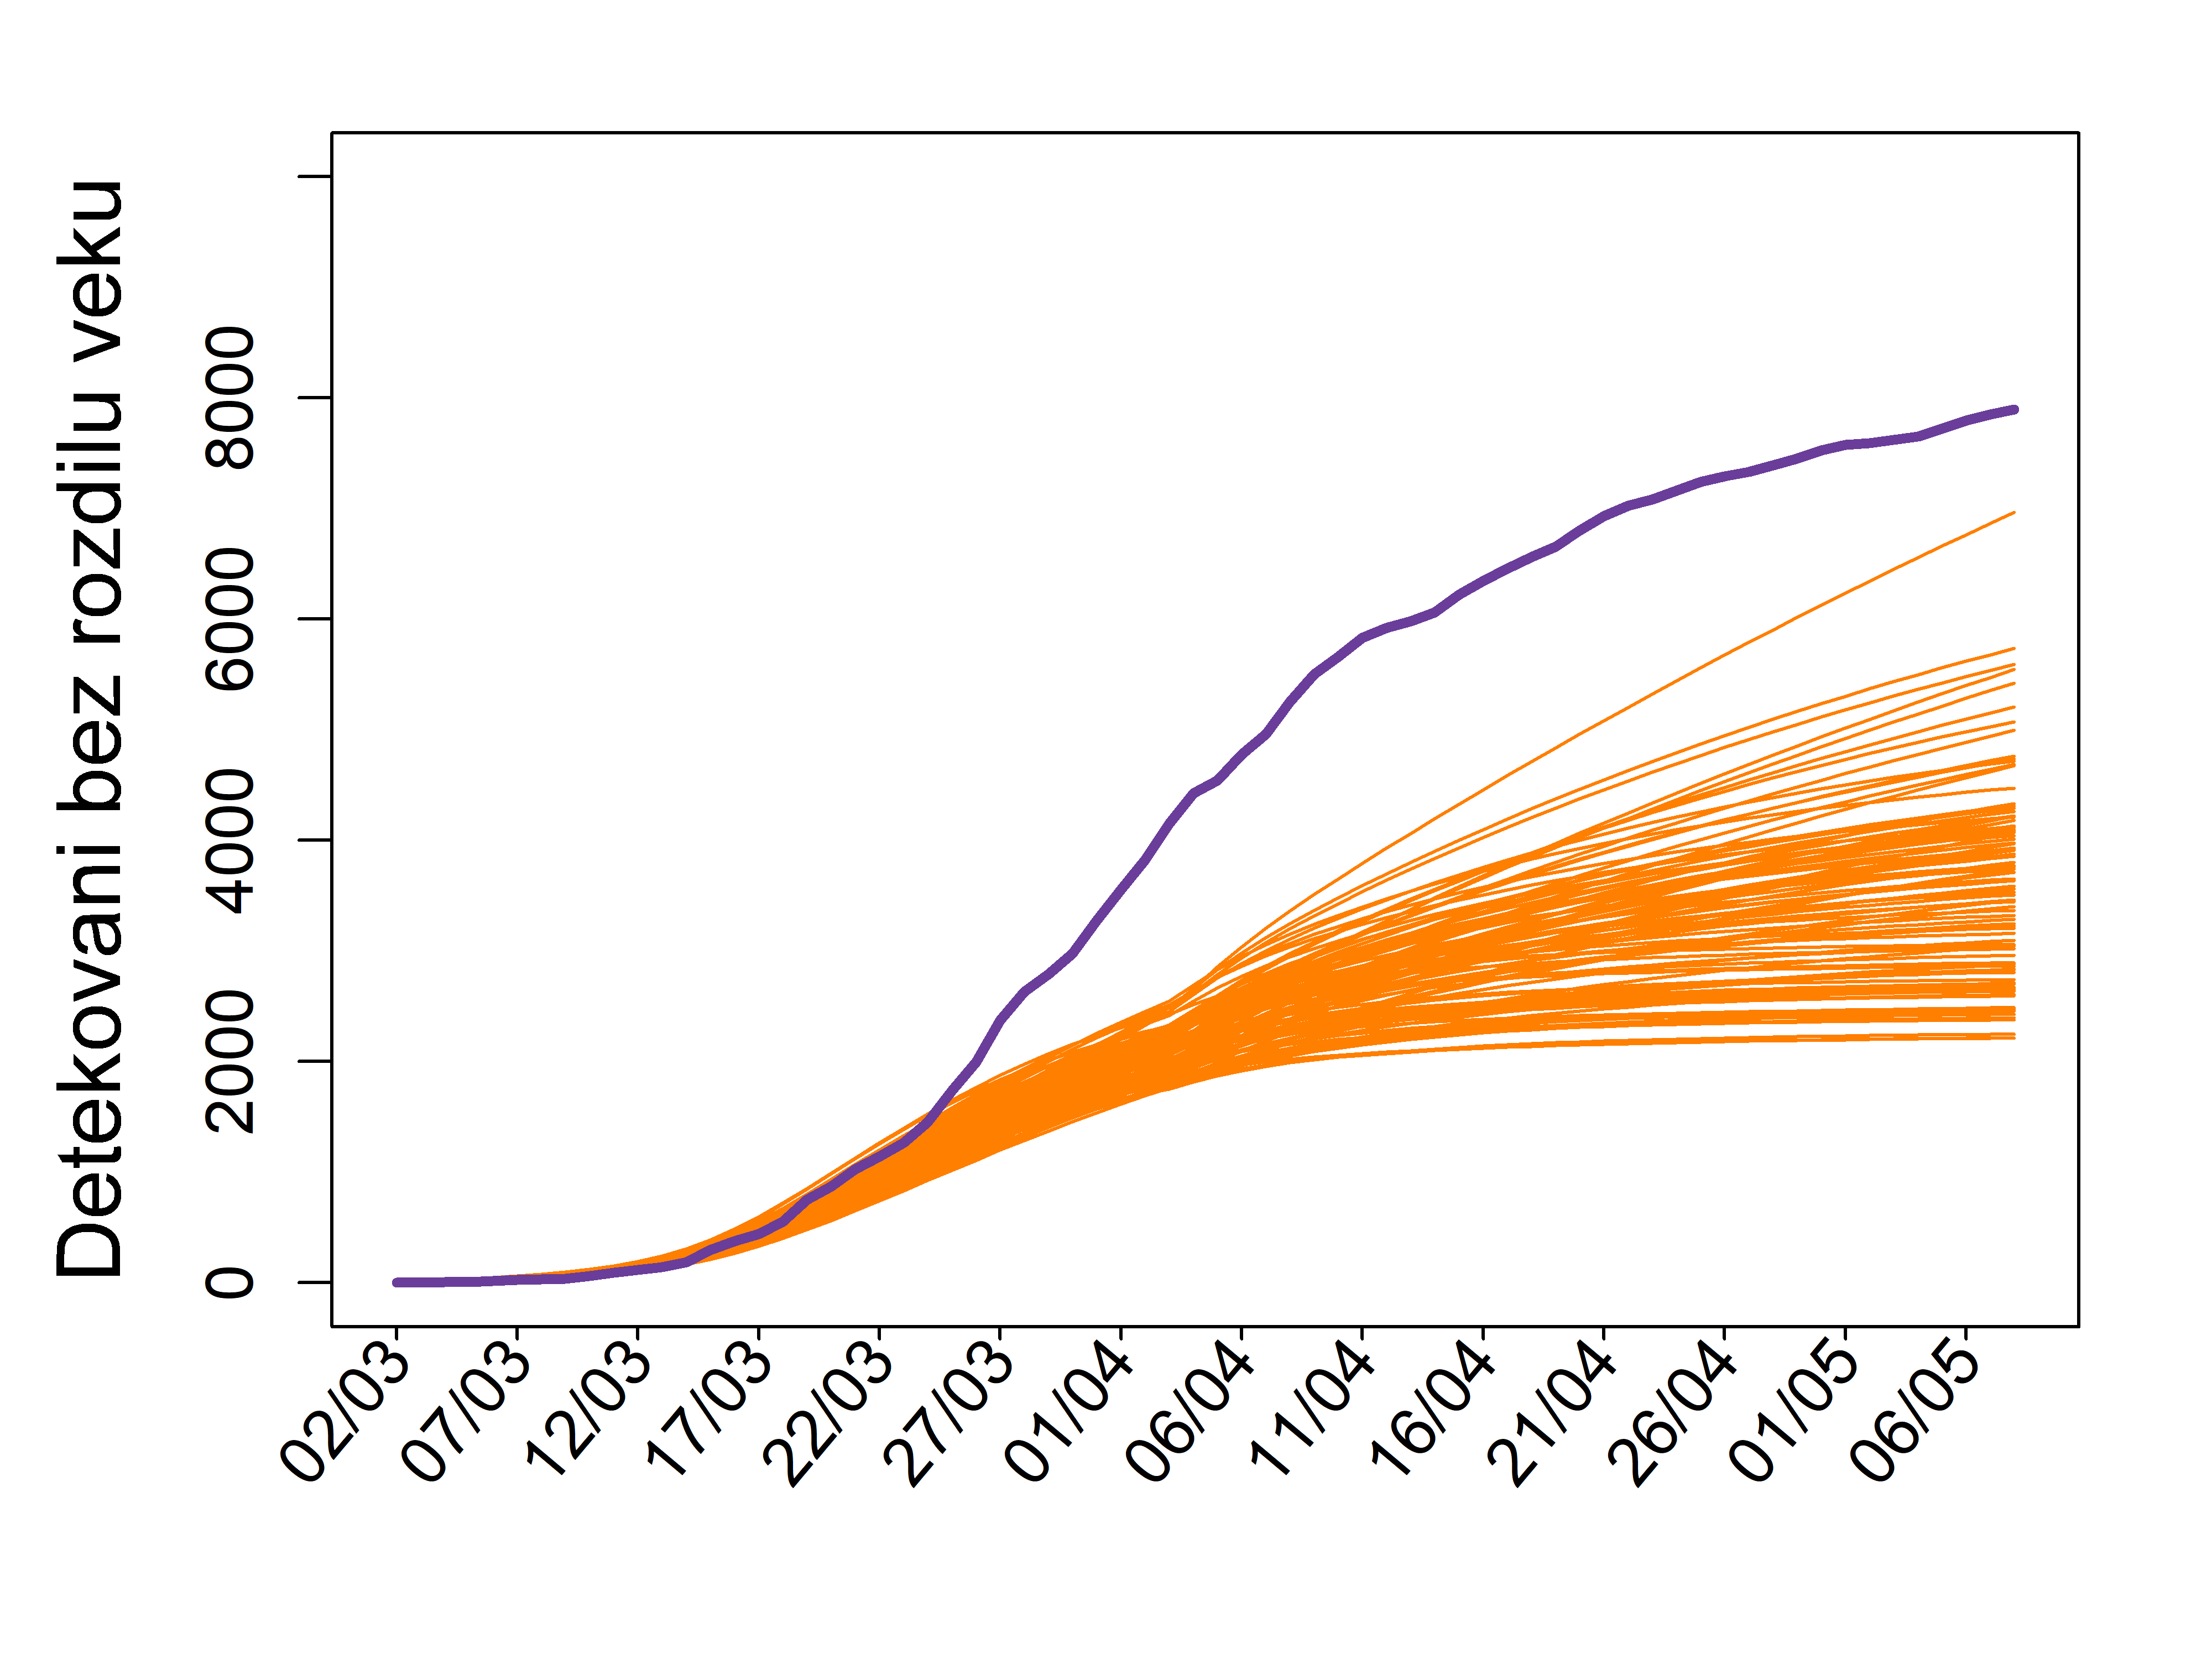
\includegraphics[width = \textwidth]{pic/sc_switch.png}
		\end{minipage}
		\begin{minipage}[m]{0.45\textwidth}
			B) \\
			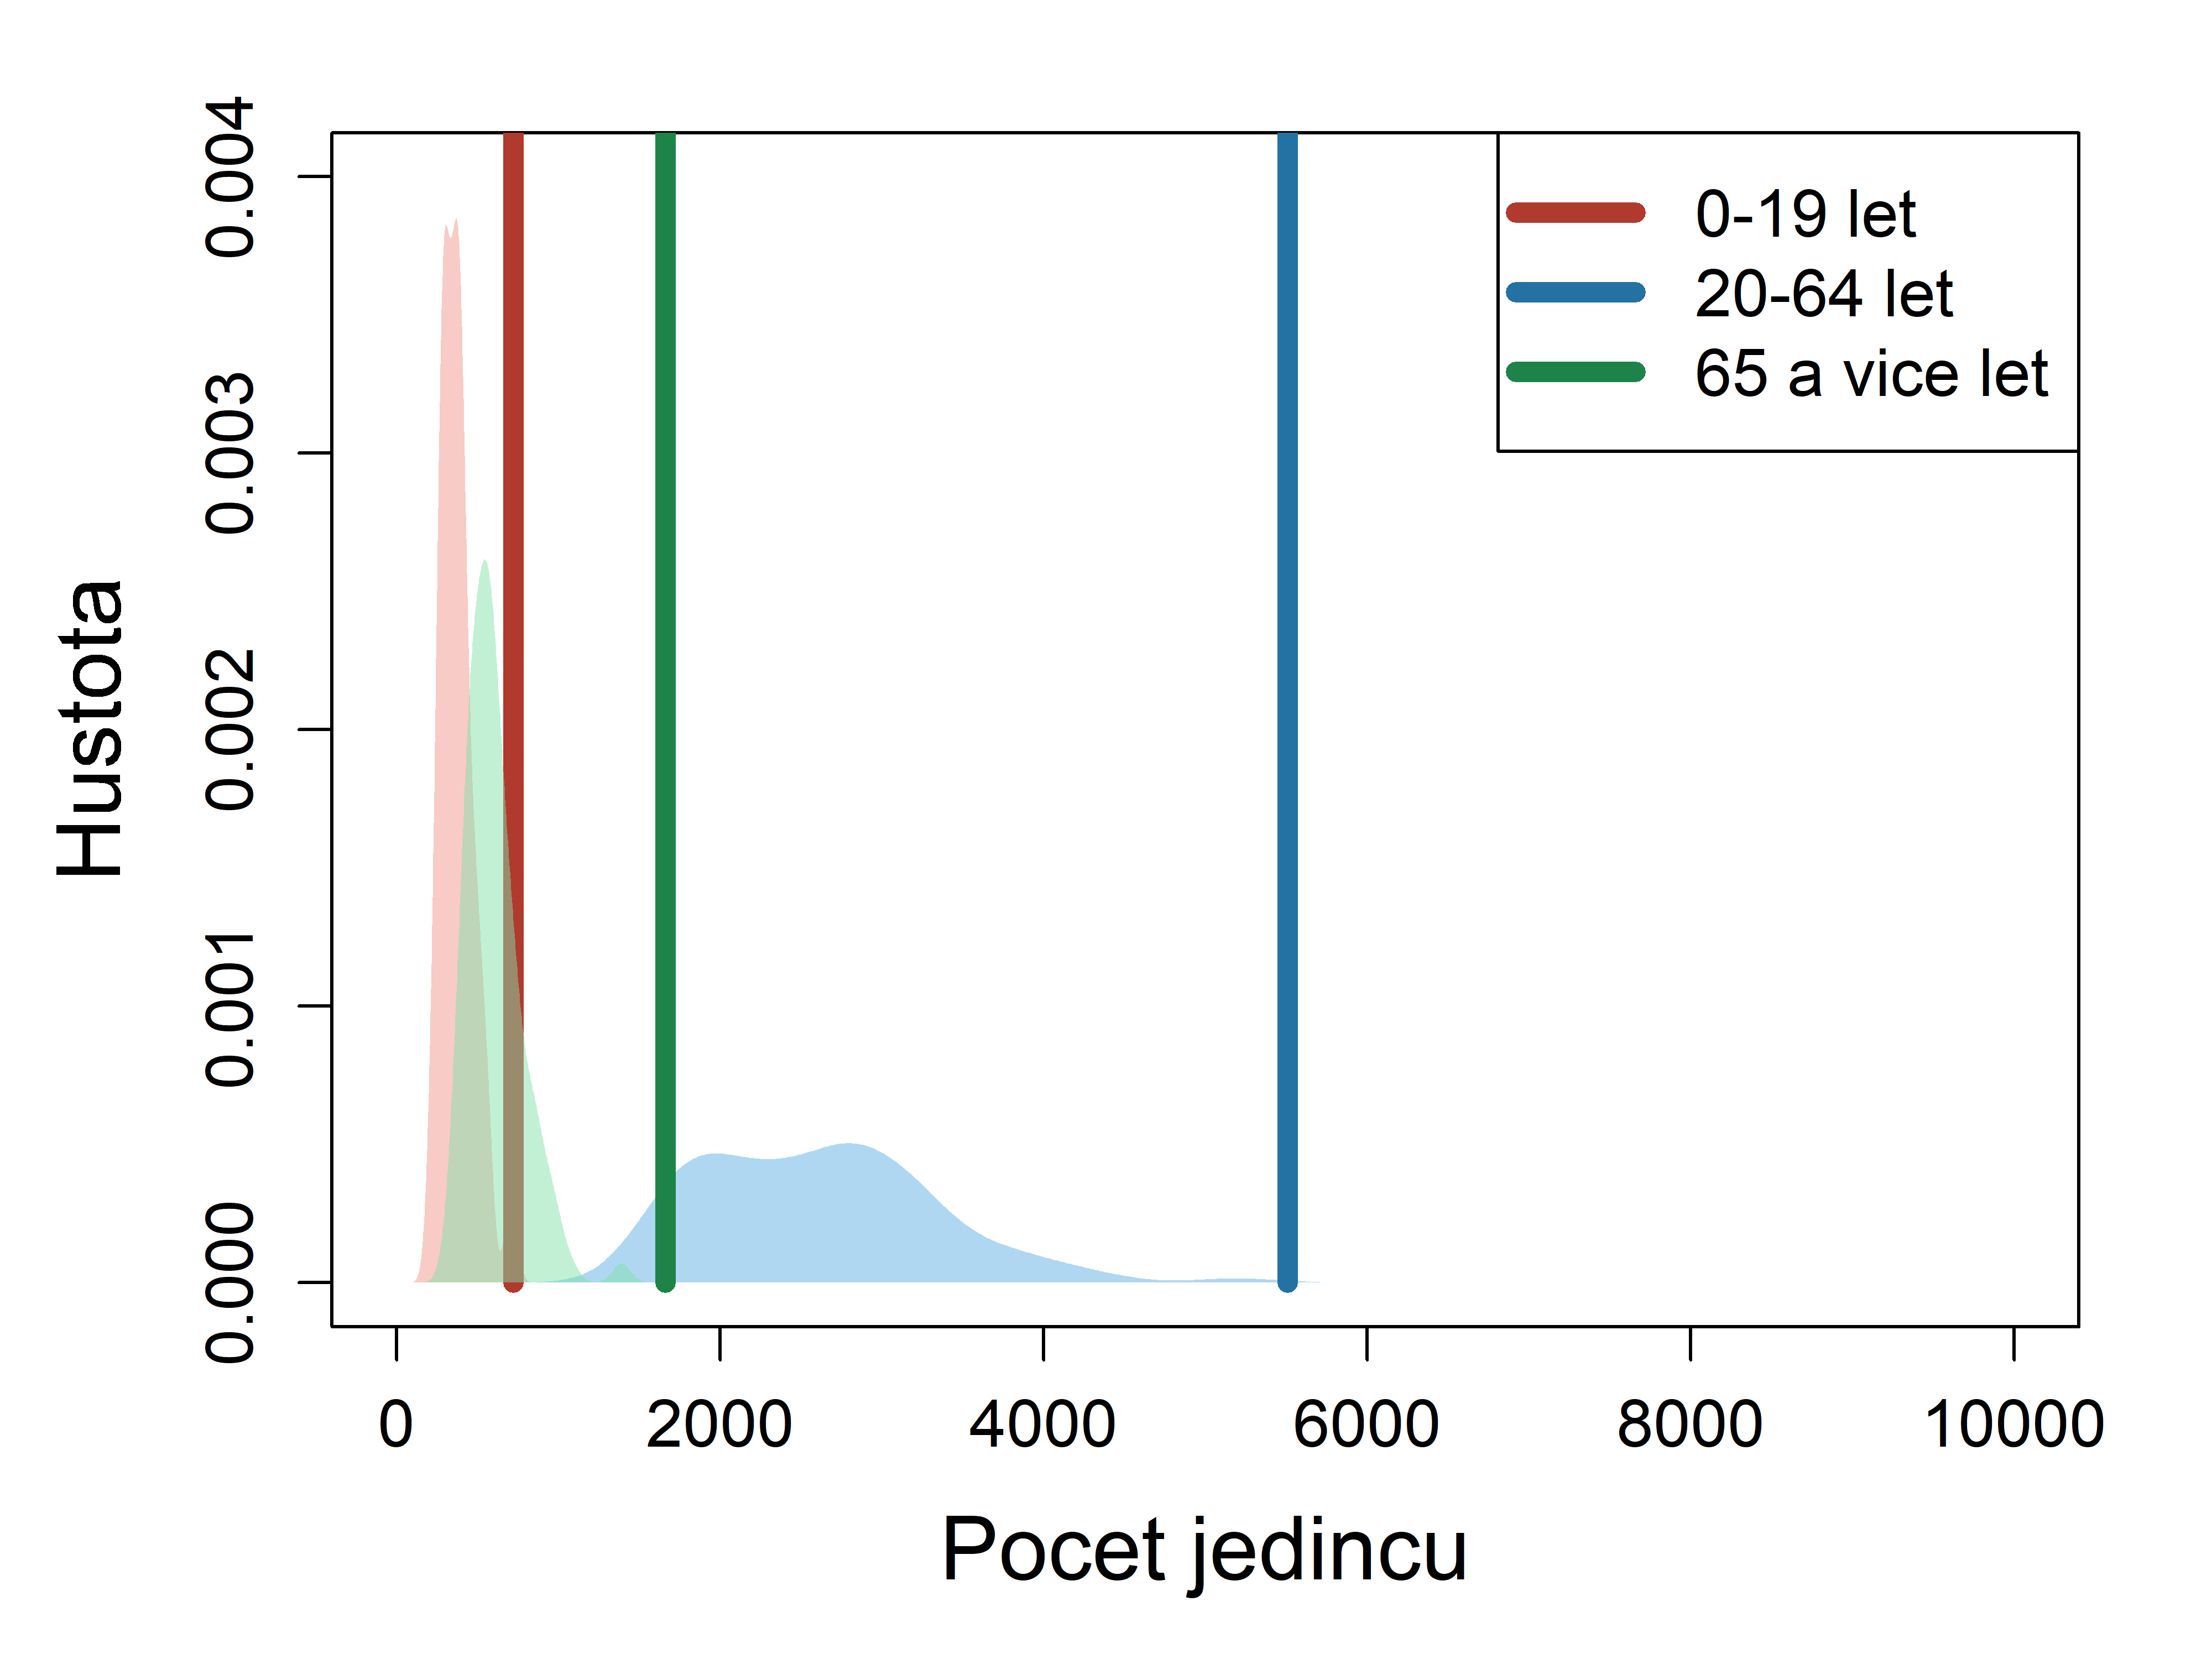
\includegraphics[width = \textwidth]{pic/sc_switch_PDF.png}
		\end{minipage} \\[1ex]
		\begin{minipage}[m]{0.45\textwidth}
			C) \\
			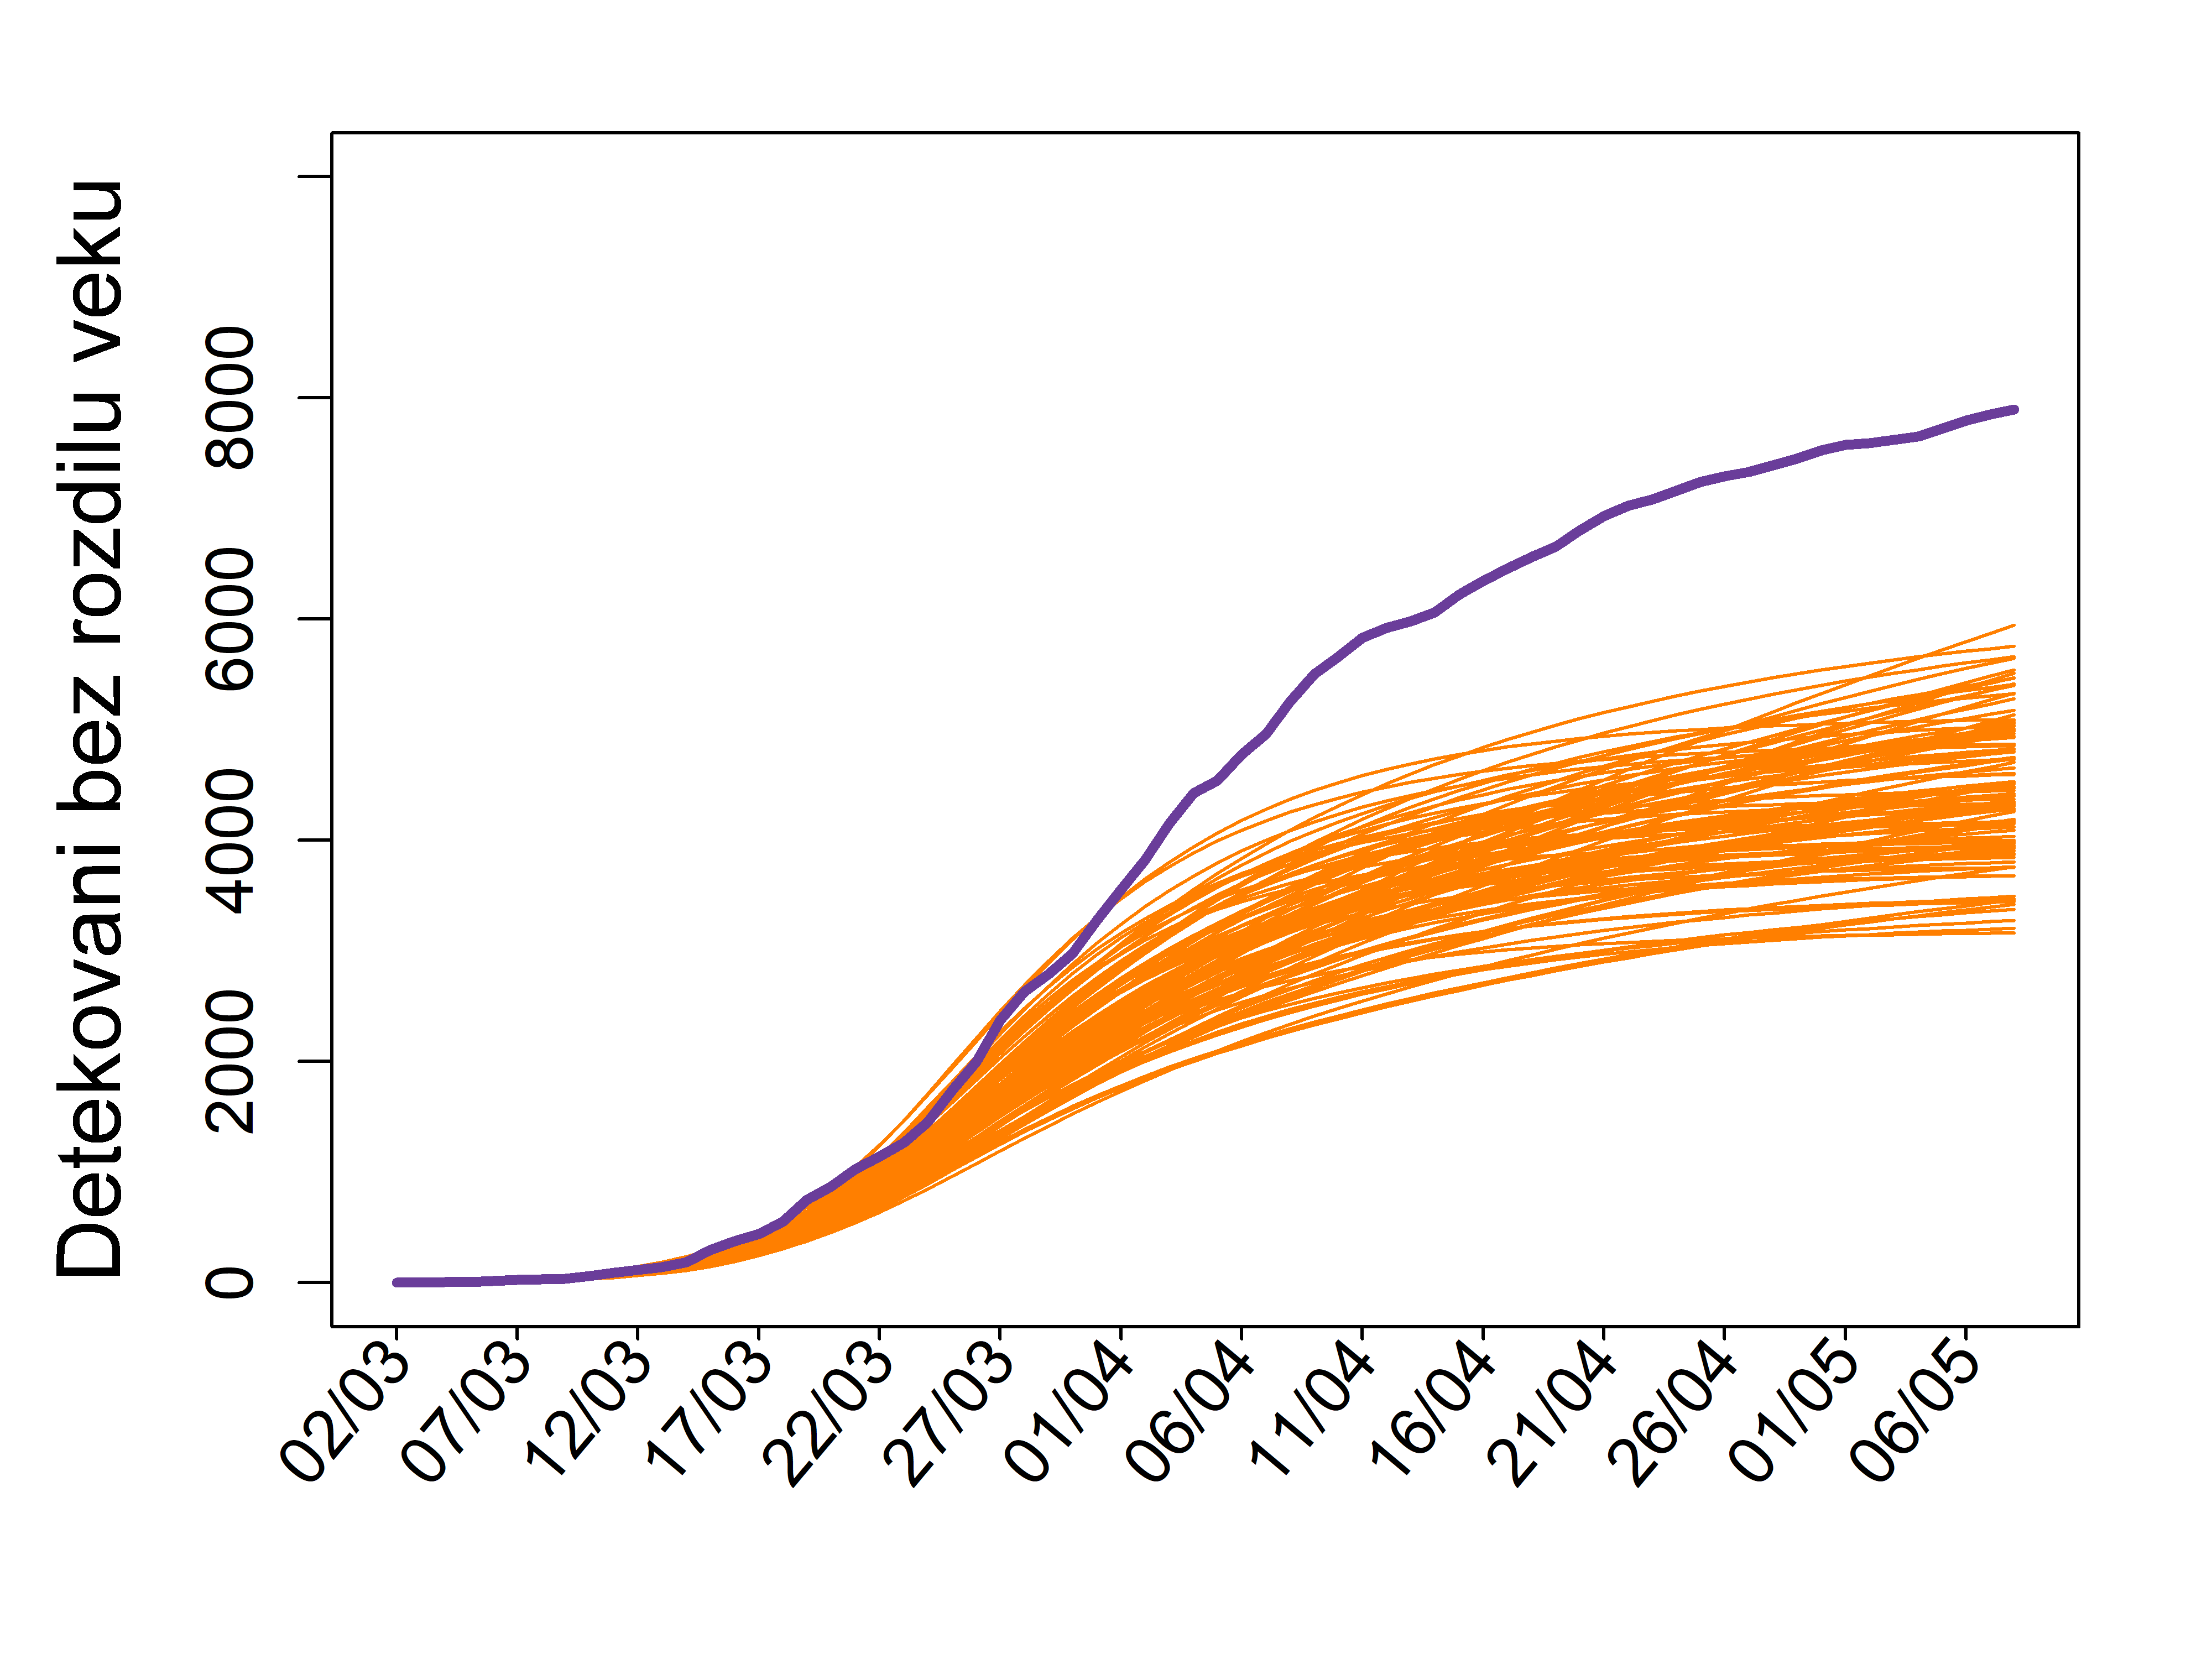
\includegraphics[width = \textwidth]{pic/sc_testing.png}
		\end{minipage}
		\begin{minipage}[m]{0.45\textwidth}
			D) \\
			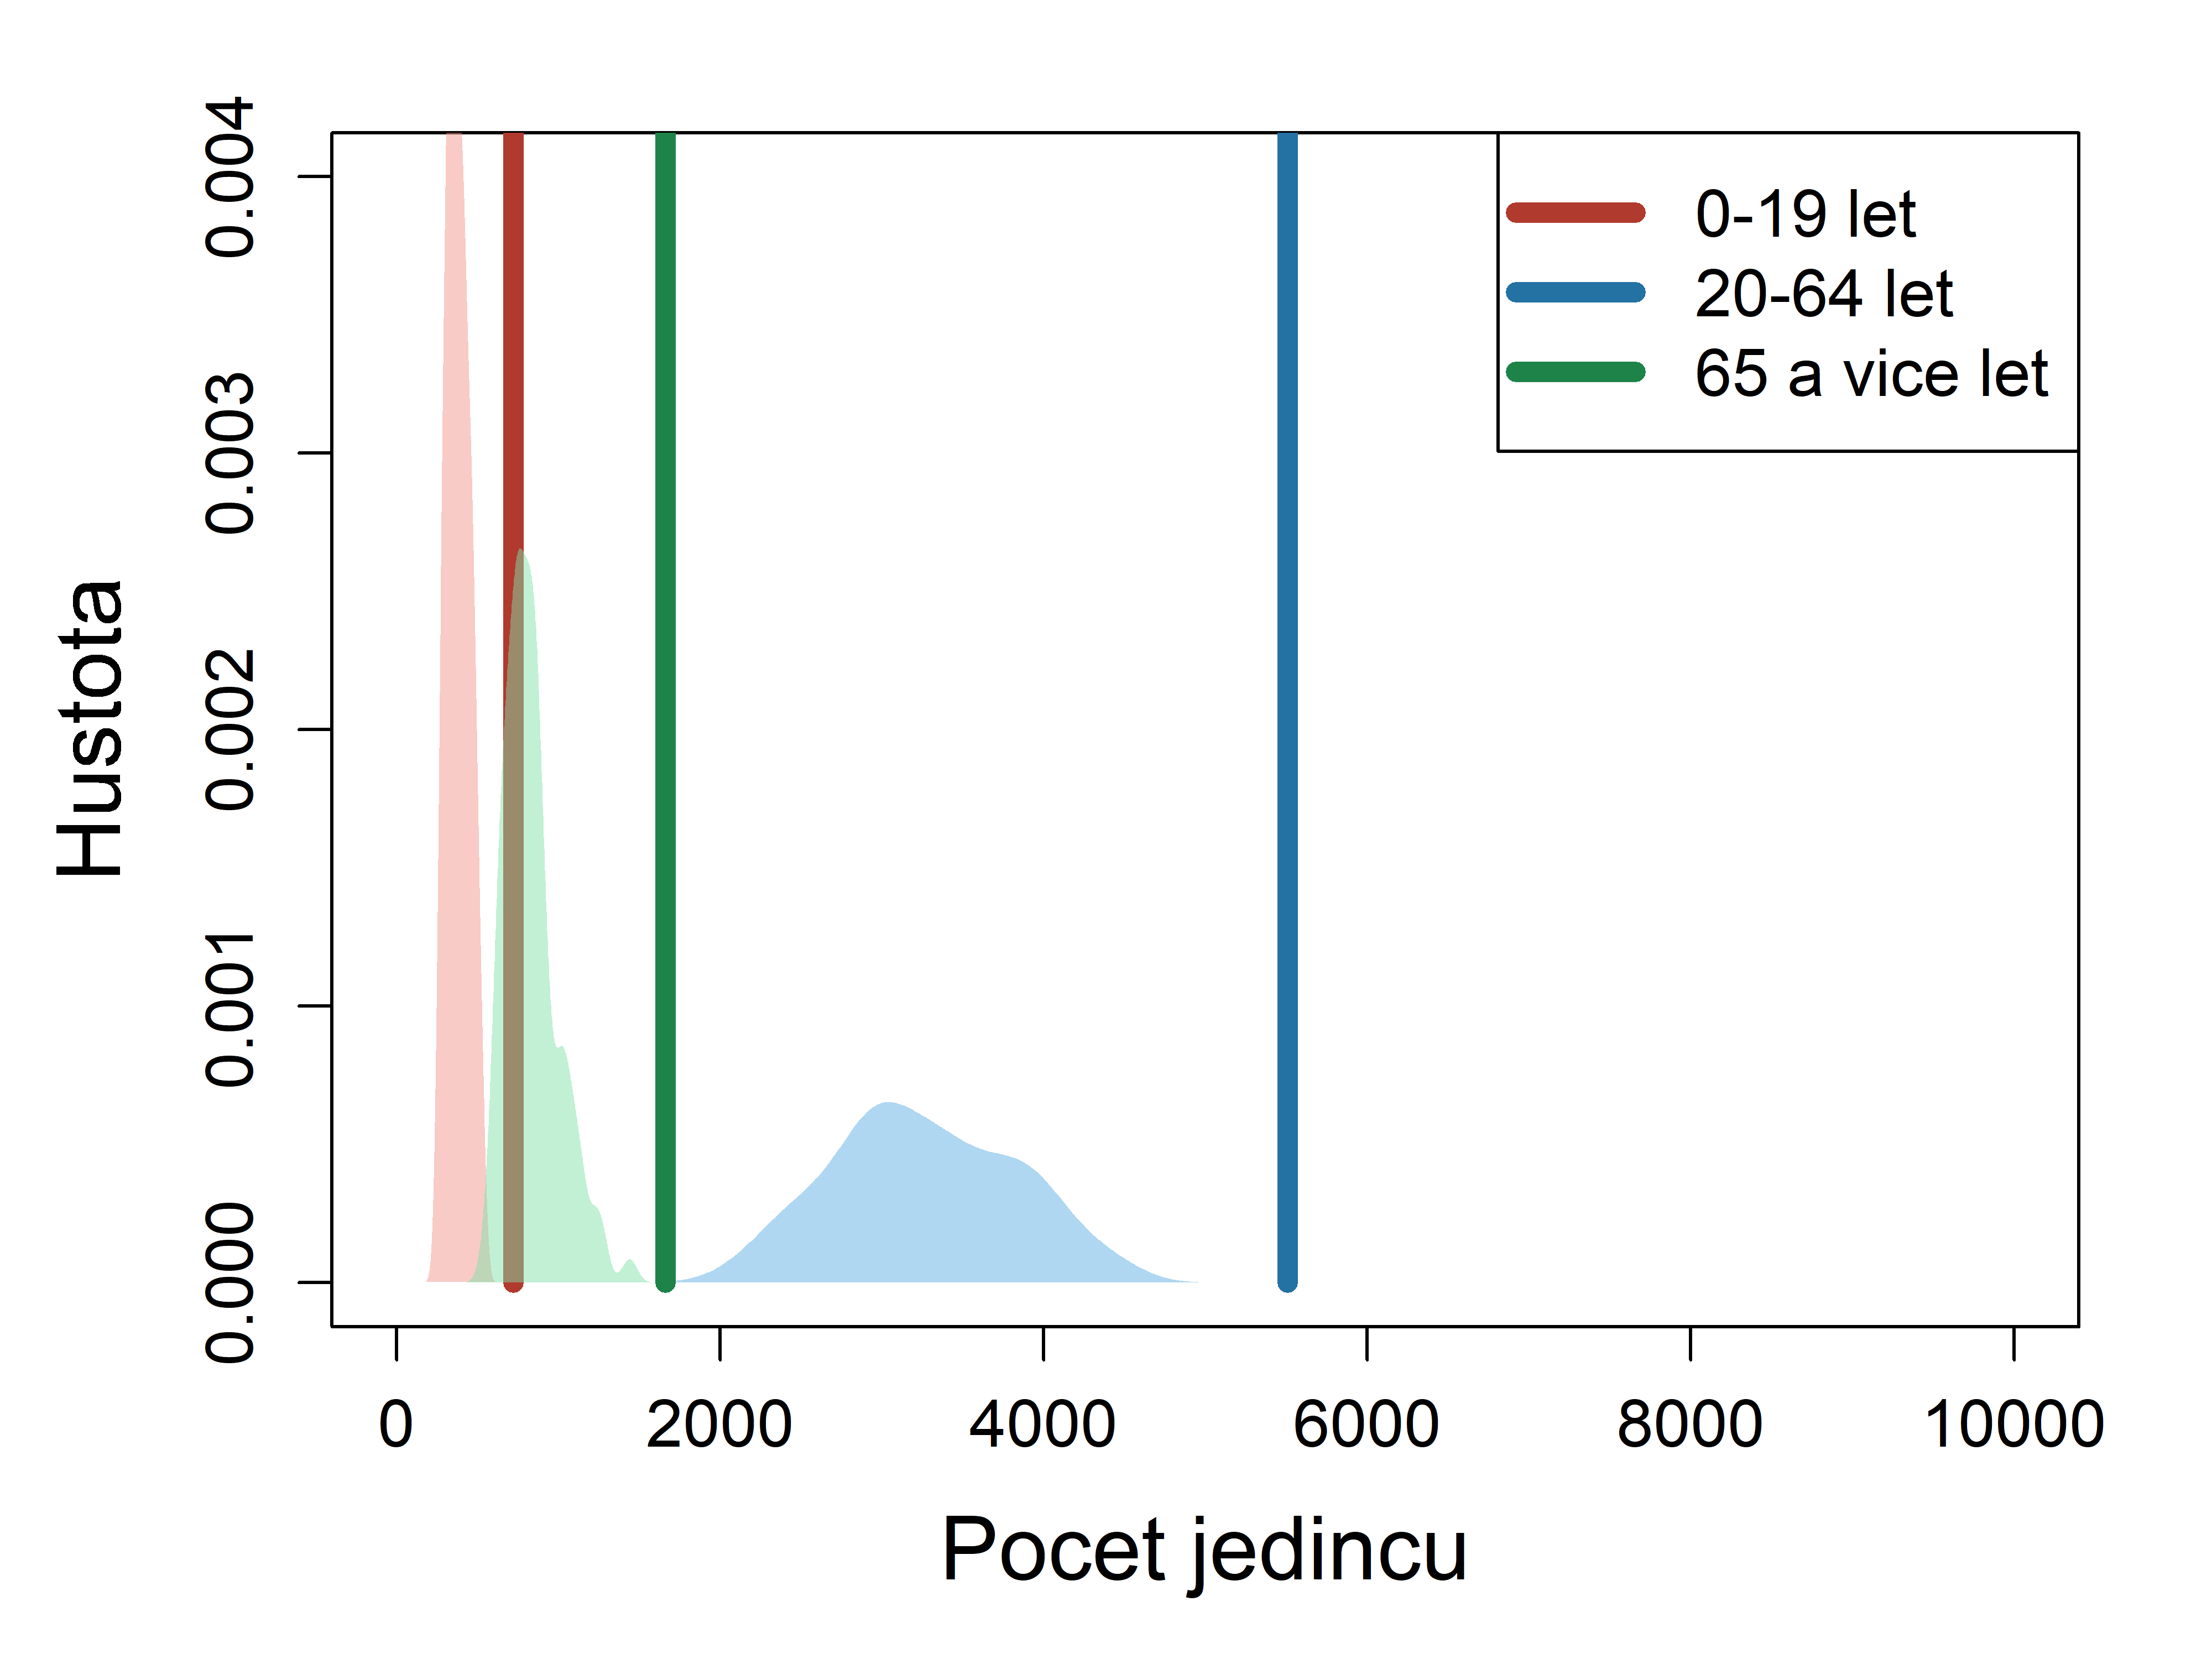
\includegraphics[width = \textwidth]{pic/sc_testing_PDF.png}
		\end{minipage}
	\end{center}
	\caption{Časová dynamika celkového počtu potvrzených případů za situace, kdy zaměníme časové okamžiky zavedení osobních ochranných opatření a zavření škol a doporučení práce z domova  (11.\ versus 19.\ března 2020, viz také tab.\,\ref{table:interventions}; panely A-B) nebo kdy po celou dobu jarní vlny uvažujeme prodlení mezi objevením se symptomů a reportováním potvrzeného případu na úrovni dubna a května 2020 (2,9 místo 6,1 dne pro březen 2020; panely C-D). Legenda jako v obr.\,\ref{scenariosR1R2}.}
	\label{switch}
\end{figure}

\section*{Závěr}

Matematické modely šíření a dopadů infekčních nemocí jsou tu s námi už více než 100 let \cite{AndersonMay1991,KeelingRohani2008,VynnyckyWhite2010}. V zásadě jakákoli infekční nemoc, která nás může napadnout, už byla velmi pravděpodobně podrobena matematickému zkoumání. Některé infekce v tom dominují, jiné jsou modelovány vzácně, nicméně téměř všechny takové modely vycházejí z filozofie a tradice založené McKendrickem a Kermackem ve 20.\ a 30.\ letech 20.\ století. Zásadní roli v této filozofii, která je shodná pro všechny typy infekcí bez ohledu na mechanismus přenosu, hrají kontakty mezi jedinci. Lapidárně řečeno, bez kontaktu není přenosu. U infekcí přenášených převážně vzduchem je samozřejmě mnohem obtížnější definovat, co to je epidemiologicky významný kontakt, na rozdíl například od pohlavně přenosných infekcí \cite{Rao_etal2021}, nicméně spojením pracovní definice, jakou například formulovala agentura PAQ Research ve svých průzkumech \cite[\url{www.zivotbehempandemie.cz}]{paqcovid}, a kalibrace modelu můžeme tuto obtíž eliminovat. Různé formy kvantifikace kontaktní struktury, jejích změn v průběhu epidemie a jejího vlivu na časový průběh epidemie si jistě v budoucnu zaslouží detailnější výzkum.

Matematické modelování má dvě zásadní role: porozumění chování modelovaného systému a předpovídání jeho chování v alespoň blízké budoucnosti, s možností manipulace systémem pro dosažení určitých cílů \cite{GerleeLundh2016}. Totéž platí o matematickém modelování v epidemiologii. Díky modelům chápeme, jak epidemie fungují, včetně objevení a role takových charakteristik jako základní a efektivní reprodukční číslo, exponenciální růst nebo práh kolektivní imunity (o tom více v kap.\,\ref{Ucinnost_ockovani}), či konkurenční dynamiky různých virových variant. Díky modelům však také umíme lépe popsat a pochopit průběhy konkrétních epidemií a prostřednictvím vyšetřování různých možných budoucích scénářů jejich další průběh cíleně ovlivnit. Není bez zajímavosti, že otázky, se kterými se setkávali vědci zabývající se modelováním infekčních nemocí v minulosti, jsou podobné těm, jaké si klademe nyní během epidemie covid-19, ať už jde o problematiku bezpečnosti vakcín či přínosu různých nefarmaceutických opatření. Ve srovnání s minulostí máme dnes mnohem sofistikovanější metody odhadu parametrů modelů z dostupných dat o časovém průběhu epidemie \cite{King_etal2016}. Schopnost položit si správnou otázku, sestavit adekvátní model reflektující dostupná data a správně interpretovat výsledky modelování však zůstává neměnná a zásadní.  

Matematičtí modeláři zažívali během pandemie covid-19 situaci, na kterou standardně nejsou zvyklí. Pod tlakem veřejnosti, médií, času, či dokonce osobních útoků se snažili nabízet pohledy na různé aspekty epidemie, zejména pak možné scénáře budoucího vývoje. Přitom své modely museli neustále modifikovat v reakci na zavádění a uvolňování různých opatření, objevení se a šíření nových a znepokojivých virových variant a v neposlední řadě v reakci na očkování. Nalezení rovnováhy mezi akademickou a veřejnou sférou z hlediska porozumění významu a výsledkům modelování infekčních nemocí je tak zcela určitě další výzvou do budoucna, spolu se schopností vědců dobře a nestranně výsledky své práce vysvětlovat veřejnosti, a to včetně nejistoty s jejich výsledky spojené, a tvůrců veřejných politik tyto výsledky respektovat a nestavět se k nim selektivně.